%/**
% * LaTeX thesis template (main file)
% * @author : Alexander willner <alex@willner.ws>
% * @url    : http://github.com/thesis
% */

% include config ---------------------------------------------------------------
\RequirePackage{pdf14}                 % PDF/A2-b compatibility
%\PassOptionsToPackage{demo}{graphicx} % for faster drafts
% document configuration -------------------------------------------------------
\documentclass[
        %pagesize,              % put paper size information into document
        a4paper,                % use a5paper for ISO A5; use a4paper for ISO A4
        pdftex,                 % PDF output
        %fontsize=12pt,         % font size
        headsepline,            % use headinclude also! (see M. Kohm)
        footsepline,            % use footinclude also! (see M. Kohm)
        %headinclude,            % count head to text body (not to margin)
        %footinclude,            % count foot to text body (not to margin)
        %BCOR8mm,               % set extra margin for book fixation
        headsepline,            % line on the top
        titlepage,              % show a title page
        %draft,                 % show under-/overfull boxes, hide images
        %demo=true,             % faster compile time
        %DIV=calc,              % calculate a nice type area
        %listof=totoc,          % List of Listings to ToC
        %oneside,               % e.g. same headings for odd and even pages
        %oneside=true,          % e.g. same headings for odd and even pages
        %twoside=false,         % e.g. same headings for odd and even pages
        %open=any,              % allows chapters to occur on left hand pages
        %openany,               % allows chapters to occur on left hand pages
        %ngerman,               % German language support
        %numbers=noendperiod    % no number at the end (German DUDEN)
%]{scrbook}
]{book}
% ------------------------------------------------------------------------------


% lang config ------------------------------------------------------------------
\usepackage[english]{babel}                  % English language support
%\usepackage[ngerman,english]{babel}         % German language support
%\usepackage{bibgerm}                        % German bibliography support
%\usepackage[babel,german=quotes]{csquotes}  % German language support
% ------------------------------------------------------------------------------


% basic packages ---------------------------------------------------------------
%\usepackage{tocloft}                         % Tweaks for large ToCs
%\cftsetpnumwidth{2em}                        % Tweaks for large ToCs
%\usepackage[demo]{graphicx}                  % faster compile time
% bugfixes ---------------------------------------------------------------------
%\let\spvec\vec                   % llncs with amsmath bugfix
%\let\vec\accentvec               % llncs with amsmath bugfix
%\newcommand{\subparagraph}{}     % IEEETrans with titlesec bugfix

%\makeatletter                    % for old listings package
%\@ifundefined{float@listhead}{}{%
%    \renewcommand*{\lstlistoflistings}{%
%        \begingroup
%            \if@twocolumn
%                \@restonecoltrue\onecolumn
%            \else
%                \@restonecolfalse
%            \fi
%            \float@listhead{\lstlistlistingname}%
%            \setlength{\parskip}{\z@}%
%            \setlength{\parindent}{\z@}%
%            \setlength{\parfillskip}{\z@ \@plus 1fil}%
%            \@starttoc{lol}%
%            \if@restonecol\twocolumn\fi
%        \endgroup
%    }%
%}
%\makeatother
% ------------------------------------------------------------------------------

% macro: ifpackageloaded -------------------------------------------------------
\makeatletter
\providecommand{\IfPackageLoaded}[2]{\@ifpackageloaded{#1}{#2}{}}
\providecommand{\IfPackageNotLoaded}[2]{\@ifpackageloaded{#1}{}{#2}}
\providecommand{\IfElsePackageLoaded}[3]{\@ifpackageloaded{#1}{#2}{#3}}
\makeatother
% ------------------------------------------------------------------------------

% File encoding: Normal UTF8 ---------------------------------------------------
\IfPackageNotLoaded{CJKutf8}{\usepackage[utf8]{inputenc}}
\usepackage[T1]{fontenc}     % Font encoding: T1
%\usepackage{cmap}           % Support copy and search for pdflatex
\input{glyphtounicode}       % Support copy and search for pdflatex % chktex 27
%\pdfgentounicode=1          % Support copy and search for pdflatex
\makeatletter
\def\UTFviii@defined#1{%
  \ifx#1\relax
      ((TODO:\@ Fix weird character here))%
  \else\expandafter% chktex 41
    #1%
  \fi
}
\makeatother
% ------------------------------------------------------------------------------

% ------------------------------------------------------------------------------
\usepackage{amssymb}                  % Springer Verlag (pdflatex)
\makeatletter
\@ifpackageloaded{url}{}{\usepackage[hyphens]{url}} % Create URLs in the document
\makeatother
\usepackage[
spacing=true,                         % Fonts: spacing?
kerning=true,
tracking=true,                        % Fonts: hyphenatable letterspacing
expansion=true,                       % Fonts: better grey value
protrusion=true]{microtype}           % Fonts: margin kerning
\microtypecontext{spacing=nonfrench}
\usepackage{textcomp}                 % For the Euro sign
\usepackage{booktabs}                 % Nice tables
\usepackage{listings}                 % Nice listings
\usepackage{listingsutf8}             % Listings with UTF-8
\lstset{columns=fullflexible,         % Listings in multicolumn mode
        breaklines=true,              % Listings with long lines
        xleftmargin=3em,              % Correct indentation
        basicstyle=\scriptsize,       % Small text
        numbers=left,                 % Show numbers
        stepnumber=1,                 % For each line
        inputencoding=utf8            % Enable UTF8
        }
\usepackage{algorithmic}              % Nice pseudo code
\makeatletter
\@ifpackageloaded{tex4ht}{%
  \usepackage[dvipdfmx]{color,graphicx}
}{
  \usepackage[table]{xcolor}                   % To use and define colors
  \usepackage{subcaption}               % Subfigures
}
\makeatother
\definecolor{LinkColor}{rgb}          % Link color
{0.31,0.46,.64}                       %
\definecolor{MarginColor}{rgb}        % Margin color
{0.31,0.46,.64}                       %
\usepackage{wrapfig}                  % Use floating images
\usepackage{stfloats}                 % Makes LaTeX honour ‘[b]’ placement
\usepackage[detect-weight=true, detect-family=true]{siunitx}  % For SI units
\usepackage{amsmath}                  % For eqref
\usepackage[olditem,oldenum]{paralist}% For inline lists (options for MDPI)
%\usepackage{fixltx2e}                 % Provides fixes for LaTeX (not needed for anymore since 2015)
\usepackage{fix-cm}                   % Provides fixes for LaTeX
\usepackage{rotating}                 % e.g. for the special side margin notes
\usepackage{lipsum}                   % To add some dummy text
\usepackage{xspace}                   % Fixing some spacing issues
\usepackage{ellipsis}                 % Puts space around ellipses
%\usepackage{ragged2e}                 % New commands/env. for setting ragged text
\usepackage{lmodern}                 % Nicer fonts (for all)
\usepackage{ltxtable}                 % Long complex tables
\usepackage{ltablex}                  % Long complex tables
\newcolumntype{L}{>{\raggedright\arraybackslash}X}
\makeatletter
\@ifpackageloaded{lineno}{}{\usepackage[switch*,modulo]{lineno}}   % Show line numbers
\makeatother
\makeatletter
\@ifpackageloaded{accsupp}{}{\usepackage{accsupp}} % Don't copy line numbers (see below)
\makeatother
\renewcommand{\thelinenumber}{        % Line number printing mechanism
  \BeginAccSupp{ActualText={}}\arabic{linenumber}\EndAccSupp{}%
}
\usepackage{blindtext}                % insert blind texts
%\usepackage{cleveref}                 % To ref footnotes twice (use after hyperref)
%\crefformat{footnote}{#2\footnotemark[#1]#3}

% on some systems, `texlive-full` does not contain accessibility.sty
% on some systems, it clashes with line numbers
% so disabling the package
%\IfFileExists{accessibility.sty}{\usepackage[tagged,highstructure]{accessibility}}{}

\makeatletter
\newcommand*{\etc}{%
    \@ifnextchar{.}%
        {etc}%
        {etc.\@\xspace}%
}
\makeatother
\newcommand*{\eg}{e.g.\@\xspace}
\newcommand*{\ie}{i.e.\@\xspace}
\newcommand*{\cf}{cf.\@\xspace}
\newcommand*{\zB}{z.\,B.\@\xspace}
\newcommand*{\zT}{z.\,T.\@\xspace}
\newcommand*{\ddh}{d.\,h.\@\xspace}
\newcommand*{\va}{v.\,a.\@\xspace}
\newcommand*{\ua}{u.\,a.\@\xspace}
\newcommand*{\uU}{u.\,U.\@\xspace}
\newcommand*{\zZ}{z.\,Z.\@\xspace}
\newcommand*{\bzw}{bzw.\@\xspace}
\newcommand*{\bspw}{bspw.\@\xspace}
\newcommand*{\ggf}{ggf.\@\xspace}
\newcommand*{\vgl}{vgl.\@\xspace}

% To be used in the project specific config file:
%\usepackage[bf]{caption}[2008/08/24]  % Bold caption (better contrast)
%\usepackage{acronym}                  % For acronyms
%\usepackage[pdftex]{graphicx}         % Include images for pdflatex

\hyphenation{op-tical net-works semi-conduc-tor con-cept}

\renewcommand{\figurename}{Fig.}
\renewcommand{\tablename}{Tab.}
\newcommand{\sectionname}{Sec.}
\newcommand{\equationname}{Eq.}
\renewcommand{\lstlistlistingname}{List of Listings}

\makeindex

\setcounter{tocdepth}{3}
\newcommand{\mykeywords}[1]{\par\addvspace\baselineskip%
\keywordname\enspace\ignorespaces#1}
\makeatletter
\providecommand*{\toclevel@title}{99}
\providecommand*{\toclevel@author}{99}

%% The tocstyle package has been withdrawn from the koma-script bundle in Juli 2020
%\usepackage[tocindentauto]{tocstyle}      % fixing large roman page letters in ToC
%\usetocstyle{standard}                    % same layout as before
%\settocstylefeature{pagenumberbox}{\hbox} % fixing large roman page letters in ToC

% type setting ----------------------------------------------------------------
% no "Schusterjungen"
    \clubpenalty=10000
% no "Hurenkinder"
    \widowpenalty=10000
    \displaywidowpenalty=10000
% type setting ----------------------------------------------------------------

% annotations --------------------------------------------------------------
\newcommand{\annot}[2][]{%
    \pdfannot\ width \linewidth\ height 2\baselineskip\ depth 0pt{%
        /Subtype/Text%
        /Open false
        /Name /Comment%
        /CA .4%
        /C [.3 .6 .9]%
        /T (\pdfescapestring{#1})%            /Contents(\pdfescapestring{\detokenize{#2}})%
    }
}

\newcommand\acc[1]{%
{%
\renewcommand{\url}[1]{}%
\renewcommand{\footnote}[1]{}%
\renewcommand{\cite}[1]{}%
\renewcommand{\nobreakspace}{}%
\let\protect\relax%
\ac{#1}%
}%
}
\newcommand\aclc[1]{%
{%
\renewcommand{\url}[1]{}%
\renewcommand{\footnote}[1]{}%
\renewcommand{\cite}[1]{}%
\renewcommand{\nobreakspace}{}%
\let\protect\relax%
\acl*{#1}%
}%
}
\newcommand\acfc[1]{%
{%
\renewcommand{\url}[1]{}%
\renewcommand{\footnote}[1]{}%
\renewcommand{\cite}[1]{}%
\renewcommand{\nobreakspace}{}%
\let\protect\relax%
\acf*{#1}%
}%
}
\newcommand\todoremark[1]{%
	\color{blue}%
	((remark: #1))
	\color{black}%
}
\newcommand\todo[1]{%
	\color{red}%
	((todo: #1))
	\color{black}%
}
\newcommand\todotext[1]{%
    \todo{#1}%
	\color[gray]{0.8}%
	\blindtext[1]
	\color{black}%
}

\newcommand\todowrite[2]{%
  \color{red}%
  ((write about #1))
	\color[gray]{0.8}%
	Lorem ipsum dolor sit amet, consectetur adipisicing elit, sed do eiusmod tempor incididunt ut labore et dolore magna aliqua. Ut enim ad minim veniam, quis nostrud exercitation ullamco laboris nisi ut aliquip ex ea commodo consequat. Duis aute irure dolor in reprehenderit in voluptate velit esse cillum dolore eu fugiat nulla pariatur.
  #2
	\color{black}%
}


\newcommand\todosmall[1]{%
    \todo{#1}%
	\color[gray]{0.8}%
	Lorem ipsum dolor sit amet, consectetuer adipiscing elit. Etiam lobortis facilisis sem. Nullam nec mi et neque pharetra sollicitudin. Praesent imperdiet mi nec ante.
	\color{black}%
}
\newcommand\todoshort[1]{\todosmall{#1}}
\newcommand\todomid[1]{%
    \todo{#1}%
    \color[gray]{0.8}%
    Lorem ipsum dolor sit amet, consectetur adipisicing elit, sed do eiusmod tempor incididunt ut labore et dolore magna aliqua. Ut enim ad minim veniam, quis nostrud exercitation ullamco laboris nisi ut aliquip ex ea commodo consequat. Duis aute irure dolor in reprehenderit in voluptate velit esse cillum dolore eu fugiat nulla pariatur.
    \color{black}%
}

\usepackage{ifoddpage}                % Move notes to correct page
\usepackage{needspace}                % Avoid hanging notes
\usepackage{marginnote,zref-savepos}  % Non floating margin notes

%\setlength{\marginparwidth}{0.7in}
\newcommand\sidenote[1]{\mbox{}%
  \marginnote{%
    \scriptsize%
    %\raggedright%
    \hspace{0pt}%
    \color{MarginColor}%
    %\begin{turn}{270}%
      \emph{#1}%
    %\end{turn}%
  }%
}%
\makeatletter
\@ifpackageloaded{tex4ht}{\renewcommand\sidenote[1]{}}{}
\makeatother

% annotations --------------------------------------------------------------

% more listings ------------------------------------------------------------
\definecolor{grey}{rgb}{0.5,0.5,0.5}
\lstdefinelanguage{sparql}{
morecomment=[l][\color{black}]{\#},
morestring=[b][\color{black}]\",
morekeywords={SELECT,CONSTRUCT,DESCRIBE,ASK,WHERE,FROM,NAMED,PREFIX,BASE,OPTIONAL,FILTER,GRAPH,LIMIT,OFFSET,SERVICE,UNION,EXISTS,NOT,BINDINGS,MINUS,a},
sensitive=true
}
\lstdefinelanguage{ttl}{
sensitive=true,
morecomment=[l][\color{grey}]{@},
morecomment=[l][\color{black}]{\#},
morestring=[b][\color{black}]\",
}
\definecolor{groovyblue}{rgb}{0,0,.9}
\definecolor{groovygreen}{rgb}{0,.7,0}
\definecolor{darkgray}{rgb}{.4,.4,.4}

\lstdefinelanguage{Groovy}[]{Java}{
  keywordstyle=\color{groovyblue}\bfseries,
  stringstyle=\color{groovygreen}\ttfamily,
  keywords=[3]{each, findAll, groupBy, collect, inject, eachWithIndex},
  morekeywords={def, as, in, use},
  moredelim=[is][\textcolor{darkgray}]{\%\%}{\%\%}, % chktex 21
  moredelim=[il][\textcolor{darkgray}]{§§}
}
% more listings ------------------------------------------------------------

% show the hex code of the unknown unicode character to actually find it ----
\usepackage{stringenc}
\usepackage{pdfescape}
\makeatletter
\renewcommand*{\UTFviii@defined}[1]{%
  \ifx#1\relax
    \begingroup
      % Remove prefix "\u8:"
      \def\x##1:{}%
      % Extract Unicode char from command name
      % (utf8.def does not support surrogates)
      \edef\x{\expandafter\x\string#1}% chktex 41
      \StringEncodingConvert\x\x{utf8}{utf16be}% convert to UTF-16BE
      % Hexadecimal representation
      \EdefEscapeHex\x\x
      % Enhanced error message
      \PackageError{inputenc}{Unicode\space char\space \string#1\space
                              (U+\x)\MessageBreak%
                              not\space set\space up\space
                              for\space use\space with\space LaTeX}\@eha%
    \endgroup
  \else\expandafter% chktex 41
    #1%
  \fi
}
\makeatother
% ---------------------------------------------------------------------------

% own requirement environment --------------------------------------------------
\makeatletter
\newcommand\requirement[3]{%
  \protected@write\@auxout{}{\string\CreateCounter{#1}}% chktex 21
  \crefname{my#1}{requirement}{requirements}\Crefname{my#1}{Requirement}{Requirements} %fixme:doesn't work
  \crefname{#1}{requirement}{requirements}\Crefname{#1}{Requirement}{Requirements} %fixme:doesn't work
  \@ifundefined{c@my#1}
    {#1??: #3}
    {\refstepcounter{my#1}\label{#2}#1\arabic{my#1}: #3}%
}
\newcommand{\CreateCounter}[1]{%
  \@ifundefined{c@my#1}
    {\newcounter{my#1}\global\@namedef{themy#1}{#1\arabic{my#1}}}% chktex 21
    {}%
}
\AtEndDocument{\let\CreateCounter\@gobble}% chktex 21
\makeatother
% ------------------------------------------------------------------------------
          % Default config
\usepackage[babel]{csquotes}                  % Biber wants it for babel
\usepackage[export]{adjustbox}                % For boxes around images
\usepackage{needspace}                        % used for embedding listings
%\usepackage{idxlayout}                       % fix index bugs and allow config
% ------------------------------------------------------------------------------

% basic config -----------------------------------------------------------------
\definecolor{LinkColor}{rgb}{0.0,0.2,0.5}     % Link color
\definecolor{MarginColor}{rgb}{0.0,0.2,0.5}   % Margin color
\definecolor{CaptionColor}{rgb}{0.0,0.2,0.5}  % Caption color
\definecolor{disabled}{gray}{0.5}             % Disabled text color
%\addtokomafont{sectioning}{\rmfamily}         % Serifs in headings
%\addtokomafont{sectioning}{\normalfont\scshape\rmfamily\color{CaptionColor}} % Serifs in headings
%\addtokomafont{sectioning}{\normalfont\rmfamily\color{CaptionColor}}        % Serifs in headings
\renewcommand{\lstlistlistingname}{List of Listings}
\renewcommand{\lstlistingname}{Listing}
\renewcommand{\contentsname}{Table of Contents}
\setcounter{secnumdepth}{4}
\setcounter{tocdepth}{2}
% basic config -----------------------------------------------------------------


% local config -----------------------------------------------------------------
\usepackage{pdflscape}
%\usepackage{subfig}
\usepackage{xmpincl}
%\includexmp{an-xmp-file-if-you-like}
\usepackage{enumitem}                   % More compact listings
\usepackage{float}                      % Provides the H float modifier option
% ------------------------------------------------------------------------------


% bibliography -----------------------------------------------------------------
\usepackage[
            style=numeric,%ieee,
            backref,
            backend=biber,
            defernumbers=true,
            useprefix=true,
            giveninits=true,
            %maxcitenames=2,
            maxbibnames=99, minbibnames=99,
            %doi=false,isbn=false,url=false,
            ]{biblatex}
\addbibresource{thesis_template.bib}
\defbibheading{empty}{}
\DeclareBibliographyCategory{cited}
\AtEveryCitekey{\addtocategory{cited}{\thefield{entrykey}}}
% ------------------------------------------------------------------------------


% acronyms ---------------------------------------------------------------------
\usepackage{acro}
\acsetup{
            single=false,
            list/sort=true,
            list/template=longtable,
            index/use, %  migh result in 'pdfTeX warning (dest): name... has been referenced but does not exist, replaced by a fixed one'
            pages/display=first,
}
\robustify\footnote%
\robustify\url%

\makeatletter\newif\ifnewacro%
\@ifpackagelater{acro}{2015/08/15}{% version 2.0 or later
\setboolean{newacro}{true}
}{% else hide footnotes and citations
\setboolean{newacro}{false}
\typeout{warning: your acro package is too old (<2.0)}
}%
\makeatother
% ------------------------------------------------------------------------------


% more config ------------------------------------------------------------------
% todo: move to 'basic config'
\usepackage{lmodern}                          % Nicer fonts (for all) - times
\usepackage{mathptmx}                         % Nicer fonts (for all) - times
%\usepackage{scrhack}                         % Fix some scrbook issues
\usepackage{scrlayer-scrpage}                 % before titlesec 
\usepackage{chapterthumb}                     % Fancy thumb index
\usepackage[chapter]{algorithm}               % Nice pseudo code
\usepackage{lettrine}                         % Drop characters, if you like
\renewcommand{\LettrineFontHook}{\color{CaptionColor}}
\usepackage[nohints]{minitoc}                 % ToC for chapters
\dominitoc[n]                                 % ToC: no caption
\renewcommand{\mtcSfont}{\small}              % ToC: small
\usepackage{makeidx}                          % Make an index
\makeindex                                    % Make an index
% ------------------------------------------------------------------------------

% chapter layout ---------------------------------------------------------------
%\usepackage[Sonny]{fncychap}                  % Nice chapter header
%\ChNameVar{\vspace*{-1in}\Large\rmfamily\vspace*{-2in}}   % Fancy chapter with serifs
%\ChTitleVar{\color{CaptionColor}\Large\rmfamily\scshape}  % Fancy chapter with serifs
\usepackage[clearempty]{titlesec}            % Suppress header and footer for empty pages
\setlength{\headheight}{1.1\baselineskip}
\titleformat{\chapter}[display]
  {\scshape\huge\color{CaptionColor}}
  {\filleft\Large\chaptertitlename~\thechapter}
  {2.5ex}
  {\titlerule\vspace{1ex}\filleft}
  [\vspace{1ex}\titlerule]
% ------------------------------------------------------------------------------

% spqueezing -------------------------------------------------------------------
%\usepackage{etoolbox}
%\makeatletter
%\patchcmd{\AC@@acro}
%  {\dotfill\pageref{acro:#1}}
%  {\nobreak\leaders\hbox{$\mkern -7mu \mkern \@dotsep mu\hbox{.}\mkern \@dotsep mu \mkern 7mu$}%
%   \hfill\nobreak\makebox[1.3em][r]{\pageref{acro:#1}}}
%  {}
%  {}
%\makeatother
% ------------------------------------------------------------------------------


% wall papger / logo on first page ---------------------------------------------
 \usepackage{wallpaper}
 \newlength\cornerXoffset%
 \newlength\cornerYoffset%
 \setlength\cornerXoffset{2cm}        % X
 \setlength\cornerYoffset{2cm}        % Y
 \newcommand\ThisLROffsetCornerWallPaper[2]{%
  \AddToShipoutPicture*{%
    \AtPageLowerLeft{%
      \parbox[b]{\paperwidth-\cornerXoffset}{%
        \hfill \includegraphics[width=#1\paperwidth,height=#1\paperheight,%
        keepaspectratio]{#2}%
        \vspace{\cornerYoffset}\null%
      }
    }
  }
 }
% ------------------------------------------------------------------------------


% page layout ------------------------------------------------------------------
%  \usepackage[ % Optional page bleed
%    cross, # some printing services might not like it others may require it...
%    center,
%    width=216mm, % A4 + 6mm
%    height=303mm % A4 + 6mm
%  ]{crop}
\usepackage[pass,a4paper]{geometry}
%\usepackage[marginparwidth=.7in, marginparsep=0.2in]{geometry}
%\geometry{a4paper, bottom=4cm}
% \renewcommand{\topfraction}{0.9}
% \renewcommand{\bottomfraction}{0.9}
% \renewcommand{\textfraction}{0.07}         % allow minimal text w. figs
% \renewcommand{\floatpagefraction}{0.7}     % require fuller float pages
% \renewcommand{\dblfloatpagefraction}{0.7}  % require fuller float pages
% \renewcommand{\dbltopfraction}{0.9}        % fit big float above 2-col. text
% \renewcommand{\textfloatsep}{5mm}
% \setcounter{topnumber}{2}
% \setcounter{bottomnumber}{2}
% \setcounter{totalnumber}{4}                % 2 may work better
% \setcounter{dbltopnumber}{2}               % for 2-column pages
% ------------------------------------------------------------------------------


% hyperlinks (almost last package) ---------------------------------------------
\usepackage{hyperxmp}                 % Semantic meta data (RDF/XMP)
%\pdfminorversion=4                   % PDF/A compatbility
%\pdfobjcompresslevel=0               % PDF/A compatbility
%\pdfcompresslevel=0                  % PDF/A compatbility
\usepackage[pdftex,                   % Hyperlinks in PDFs
pdfa=true,                            % PDF/A compatbility (fix hyperlink with ghostscript)
pdfapart=1,                           % PDF/A compatbility
unicode=true,                         % PDF/A compatbility
raiselinks=true,			                % calculate real height of the link
breaklinks,                           % break links
%backref=page,                        % backlinks in bibliography (section, slide, page, none)
%pagebackref=true,                    % backlinks in bibliography
hyperindex=true,                      % backlinkex index
linktocpage=true,                     % ToC links pages
bookmarks=true,                       % Bookmarks for PDF viewers
bookmarksopen=true,                   % Open bookmarks
bookmarksopenlevel=2,                 % How many levels to open
bookmarksnumbered=true,               % Numbers in the bookmarks
bookmarkstype=toc,                    % Type of bookmark
plainpages=false,                     % Anchors even on plain pages?
pageanchor=true,                      % Pages are linkable
pdfstartview=FitH,                    % Open document with Fit Width
pdfpagelabels=true,                   % set PDF page labels
pdfpagemode=UseOutlines,              % Show bookmarks in viewer
colorlinks,                           % Show colored links
linkcolor=LinkColor,                  % Link color
urlcolor=LinkColor,                   % URL color
anchorcolor=LinkColor,                % Anchor color
citecolor=LinkColor,                  % Cite color
menucolor=LinkColor,                  % Menu color
hypertexnames=true                    % Whatever ;)
]{hyperref}                           % Use hyperlinks
%\renewcommand*{\backref}[1]{[cited at page #1]} % Show formatted backlinks
\usepackage{bookmark}                 % Manually add PDF bookmarks
\hypersetup{keeppdfinfo}              % fix for hyperxmp, however, breaks PDF/A compliance
% ------------------------------------------------------------------------------


% cleveref with fixes ----------------------------------------------------------
\usepackage{cleveref}                 % To ref footnotes twice (use after hyperref)
\crefformat{footnote}{#2\footnotemark[#1]#3}
% ------------------------------------------------------------------------------


% glossary (last package) ----------------------------------------------------
\usepackage[xindy,nonumberlist,toc]{glossaries}
\newglossaryentry{Term}
{
  name=Term,
  description={A general-purpose term}
}
\newglossaryentry{Foo}
{
    name={Foo},
    description={Bar}
}

\setglossarystyle{altlist}
\renewcommand*{\glsgroupskip}{}
\makeglossaries%
% ------------------------------------------------------------------------------


% meta data --------------------------------------------------------------------
% meta data --------------------------------------------------------------------
\newcommand{\metaType}{M.Sc of Computer Science}
\newcommand{\metaTypeShort}{M.Sc.CS.}
\newcommand{\metaWhy}{To get the degree in}
\newcommand{\metaHowFinal}{Submitted}
\newcommand{\metaHowNonFinal}{Draft}
\newcommand{\metaBoard}{Board}
\newcommand{\metaSubmitted}{Presented by}
\newcommand{\metaDate}{16.~June~2023}
\newcommand{\metaDateEn}{16.~June~2020}
\newcommand{\metaDateExam}{\metaDate}
\newcommand{\metaNumber}{2020--06}
\newcommand{\metaTitleLayouted}{Proposal:\\A flow-aware multipath tunnel implementation\\based on AF\_XDP socket}
\newcommand{\metaTitle}{Sophisticated Template for a Thesis}
\newcommand{\metaTitleShort}{Thesis Template}
\newcommand{\metaDegree}{B.Sc}
\newcommand{\metaBirthplace}{Born in Foo Bar}
\newcommand{\metaAuthor}{Ba Que, Le}
\newcommand{\metaAuthorMail}{first.last@example.org}
\newcommand{\metaKeywords}{Foo, Bar, First, Last}
\newcommand{\metaSubject}{Template Subject}
\newcommand{\metaUniversity}{Technical University of Berlin}
\newcommand{\metaFaculty}{Chair of Next Generation Networks (AV) }
\newcommand{\metaDepartment}{Template Department}
\newcommand{\metaCitycode}{12345}
\newcommand{\metaCity}{City}
\newcommand{\metaCountry}{Country}
\newcommand{\metaURL}{http://example.org}
\newcommand{\metaChair}{Chair}
\newcommand{\metaChairName}{Prof. Dr. Thomas Magedanz}
\newcommand{\metaChairUniversity}{Technical University of Berlin}
\newcommand{\metaReviewer}{Reviewer}
\newcommand{\metaFirstReviewerName}{Prof.\ Dr.-Ing.\ Foo Bar}
\newcommand{\metaFirstReviewerUniversity}{Example University}
\newcommand{\metaSecondReviewerName}{Prof.\ Dr.\ Bar Foo}
\newcommand{\metaSecondReviewerUniversity}{Another University}
\newcommand{\metaThirdReviewerName}{Dr.\ John Smith}
\newcommand{\metaThirdReviewerUniversity}{My University}
\newcommand{\metaFourthReviewerName}{{\color{gray}Dr.\ Jon Doe}}
\newcommand{\metaFourthReviewerUniversity}{{\color{gray}BAR}}


\newcommand{\metaAuthorShort}{\metaAuthor}
\newcommand{\metaConference}{Conference}
\newcommand{\metaConferenceArea}{Area}
\newcommand{\metaDedication}{\scriptsize{Dedicated to my beloved family.}}
% ------------------------------------------------------------------------------

% % meta data --------------------------------------------------------------------
% \newcommand{\metaType}{PhD of templates}
% \newcommand{\metaTypeShort}{Dr.-Tmpl.}
% \newcommand{\metaWhy}{To get the degree in}
% \newcommand{\metaHowFinal}{Submitted}
% \newcommand{\metaHowNonFinal}{Draft}
% \newcommand{\metaBoard}{Board}
% \newcommand{\metaSubmitted}{Presented by}
% \newcommand{\metaDate}{16.~Juni~2020}
% \newcommand{\metaDateEn}{16.~June~2020}
% \newcommand{\metaDateExam}{\metaDate}
% \newcommand{\metaNumber}{2020--06}
% \newcommand{\metaTitleLayouted}{Sophisticated Template\\for a Thesis}
% \newcommand{\metaTitle}{Sophisticated Template for a Thesis}
% \newcommand{\metaTitleShort}{Thesis Template}
% \newcommand{\metaDegree}{MTA}
% \newcommand{\metaBirthplace}{Born in Foo Bar}
% \newcommand{\metaAuthor}{First Last}
% \newcommand{\metaAuthorMail}{first.last@example.org}
% \newcommand{\metaKeywords}{Foo, Bar, First, Last}
% \newcommand{\metaSubject}{Template Subject}
% \newcommand{\metaUniversity}{Template University}
% \newcommand{\metaFaculty}{Template Faculty}
% \newcommand{\metaDepartment}{Template Department}
% \newcommand{\metaCitycode}{12345}
% \newcommand{\metaCity}{City}
% \newcommand{\metaCountry}{Country}
% \newcommand{\metaURL}{http://example.org}
% \newcommand{\metaChair}{Chair}
% \newcommand{\metaChairName}{Prof.\ Dr.-Ing.\ Goo Gl}
% \newcommand{\metaChairUniversity}{Industry}
% \newcommand{\metaReviewer}{Reviewer}
% \newcommand{\metaFirstReviewerName}{Prof.\ Dr.-Ing.\ Foo Bar}
% \newcommand{\metaFirstReviewerUniversity}{Example University}
% \newcommand{\metaSecondReviewerName}{Prof.\ Dr.\ Bar Foo}
% \newcommand{\metaSecondReviewerUniversity}{Another University}
% \newcommand{\metaThirdReviewerName}{Dr.\ John Smith}
% \newcommand{\metaThirdReviewerUniversity}{My University}
% \newcommand{\metaFourthReviewerName}{{\color{gray}Dr.\ Jon Doe}}
% \newcommand{\metaFourthReviewerUniversity}{{\color{gray}BAR}}


% \newcommand{\metaAuthorShort}{\metaAuthor}
% \newcommand{\metaConference}{Conference}
% \newcommand{\metaConferenceArea}{Area}
% \newcommand{\metaDedication}{\scriptsize{Dedicated to my beloved family.}}
% % ------------------------------------------------------------------------------

%%% Only for koma script
%\subject{\metaSubject}
%\title{\metaTitle}
%\author{\metaAuthor}
%\date{\metaDate}
%\dedication{\metaDedication}

\hypersetup{
      pdfauthor={\metaAuthorShort~<\metaAuthorMail>},
      pdfsubject={\metaSubject},
      pdftitle={\metaTitle},
      pdfkeywords={\metaKeywords},
      pdfcreator={http://github.com/tubav/},
      pdfproducer={pdfTeX},
}

% ------------------------------------------------------------------------------


% final fixes ------------------------------------------------------------------
\righthyphenmin=2
\tolerance=2000
\emergencystretch=10pt
% ------------------------------------------------------------------------------

% PDF/A color profile ----------------------------------------------------------
\immediate\pdfobj stream attr{/N 3}  file{lib/resources/pdfa/srgb.icc}% chktex 1
\pdfcatalog{%
/OutputIntents [ <<
/Type /OutputIntent
/S/GTS_PDFA1
/DestOutputProfile \the\pdflastobj\space 0 R
/OutputConditionIdentifier (sRGB IEC61966-2.1)% chktex 8
/Info(sRGB IEC61966-2.1)% chktex 8 chktex 36
>> ]
}
% ------------------------------------------------------------------------------
     % inlcude general configuration
\DeclareAcronym{ABAC}{short={ABAC}, long={Attributed Based Access Control}, cite={li2002design,Yuan2005}}
\DeclareAcronym{DBpedia}{short={DBpedia}, long={DBpedia}, cite={Auer2007}, long-post={\acroiffirstT{\footnote{\url{http://dbpedia.org}}}}, first-style = long, tag=exclude}
%\DeclareAcronym{PLC}{short={PLC}, long={Programmable Logic Controller}}
%\DeclareAcronym{}{short={}, long={}}
%\DeclareAcronym{}{short={}, long={}, short-indefinite={an},  long-indefinite={an}, cite={}, long-post={\acroiffirstT{\footnote{\url{https://}}}}, first-style = long, tag=exclude}
%\DeclareAcronym{Swoogle}{short={Swoogle}, long={}, cite={ding2004swoogle}, long-post={\acroiffirstT{\footnote{\url{http://swoogle.umbc.edu}}}}}
       % inlcude acronyms
\DeclareUnicodeCharacter{0301}{}       % fixing an UTF-8 encoding issue
%\usepackage[norefs,nocites]{refcheck} % useful, but not working with cref
%\usepackage[doublespacing]{setspace}  % useful for reviewing a printout
%\PassOptionsToPackage{cmyk}{xcolor}   % PDF/A compatibility, skipped
%\usepackage[a-2b]{pdfx}               % PDF/A compatibility, skipped
\newcommand{\isFinal}{true}            % Modify e.g. the title page
\AddLayersToPageStyle{@everystyle@}{chapterthumb}
\addtokomafont{chapterthumb}{\bfseries}
% ------------------------------------------------------------------------------


% include only required files for faster building ------------------------------
%\includeonly{src/03_requirements,src/06_implementation}
% ------------------------------------------------------------------------------


% begin thesis -----------------------------------------------------------------
\begin{document}
    \frontmatter
    \pagestyle{empty}
    \pagenumbering{alph}
    \pdfbookmark{Title}{title}
\begin{titlepage}
\newgeometry{left=35mm, right=35mm, top=35mm, bottom=35mm}


\begin{center}
\vspace*{2cm}
\LARGE{\metaTitleLayouted}\\
\normalsize

\vspace*{2cm}
\metaSubmitted%
\\
\metaAuthor, \metaDegree~\\
\metaBirthplace%
\\

\vspace*{2cm}
\metaFaculty%
\\
\metaUniversity%
\\
\metaWhy%
\\
\vspace*{0,5cm}
\metaType%
\\
-~{\metaTypeShort}~-% chktex: 8
\\
\vspace*{0,5cm}

\ifthenelse{\equal{\isFinal}{true}}{
\metaHowFinal%
}{
\metaHowNonFinal%
}
\end{center}

\ifthenelse{\equal{\isFinal}{true}}{

\vspace*{2cm}
\metaBoard:\\
\vspace*{.3cm}\\
\begin{tabular}{@{\hspace{1.5em}}ll}
\metaChair: & \metaChairName~(\metaChairUniversity) \\
\metaReviewer: & \metaFirstReviewerName~(\metaFirstReviewerUniversity) \\
\metaReviewer: & \metaSecondReviewerName~(\metaSecondReviewerUniversity)\\
\metaReviewer: & \metaThirdReviewerName~(\metaThirdReviewerUniversity)\\
\end{tabular}

\vspace*{1,9cm}
\metaDateExam%
\vspace*{0,9cm}

}{
\vspace*{6cm}
}

\begin{center}
\metaNumber\newline
\end{center}


\ThisLROffsetCornerWallPaper{.2}{resources/images/logo}   % logo in the corner

\restoregeometry%
\end{titlepage}

    % \cleardoublepage\vspace*{100mm}
\begin{minipage}{109.5mm}
\section*{Affidavit}
I hereby declare that the following thesis ``\metaTitle'' has been
written only by the undersigned and without any assistance from third
parties.\\

Furthermore, I confirm that no sources have been used in the preparation
of this thesis other than those indicated in the thesis itself.\\[2cm]
\metaCity,
\metaDate%
\end{minipage}

    % \cleardoublepage\pdfbookmark{Dedication}{dedication}
\begin{center}
\LARGE{\metaDedication}
\end{center}

    %\cleardoublepage

    \pagestyle{scrheadings}
    %\lohead[]{}
    \pagenumbering{roman}
    \setcounter{page}{1}
    % \pdfbookmark{Acknowledgments}{acknowledgments}
\chapter*{Acknowledgments}

\todomid{thank your supervisors}

\todomid{thank your colleagues}

\todomid{thank your family and friends}

\vspace{0.5in}
\begin{flushright}
  \metaCity, June 16, 2020%\today%
\end{flushright}
\cleardoublepage{}
    \pdfbookmark{Abstract}{abstract}
\chapter*{Abstract}

Tunneling refers to the method of securely and isolatedly transferring network packets between two hosts over a public network, often without revealing their actual addresses to the applications. 
This is achieved by encapsulating the real traffic of the application before sending it, and then unwrapping before delivering to the associated virtual addresses.
The flow of packets in tunneling is comparable to the movement of vehicles through a tunnel, hence the analogy. Various tunnel protocols exist, ranging from high-level protocols like SSH tunneling at the application layer to lower-level protocols like IPsec at the network layer, and PPTP, PPPoE, and L2TP at the link layer.
The implementation of multipath tunneling can outperform traditional single-line solutions in terms of performance factors such as bandwidth, reliability, and latency.
This document will explore the concept of multipath tunneling and present a low-level implementation using the eBPF-based AF\_XDP socket, which is known for its maximum performance and system reliability.
The results of this project can serve as a proof of concept and lay the groundwork for further research on algorithms and protocols, as well as applications such as overhauling the 5G core network.

% {\setlength{\parindent}{-.1cm}%
% \sidenote{Research Area:\\Foo Bar}%
% \todomid{write about the research area}

% \sidenote{Application Area:\\Bar Foo}
% \todomid{write about the application area}

% \sidenote{Research Issue:\\Foo Fooli}
% \todomid{write about the research issue}

% \sidenote{Own Approach:\\Bar Barli}
% \todomid{write about the own approach}

% \sidenote{Scientific Contributions}
% \todomid{write about the scientific contributions}

% \sidenote{Validation \& Outlook}
% \todomid{write about the validation and outlook}

% \cleardoublepage
% \begin{otherlanguage}{ngerman}
% \pdfbookmark{Zusammenfassung}{Zusammenfassung}
% \chapter*{Zusammenfassung}%

% \sidenote{For\-schungs\-be\-reich:\\Foo Bar}%
% \todomid{write}

% \sidenote{Ein\-grenz\-ung:\\Bar Foo}
% \todomid{write}

% \sidenote{Pro\-blem\-stel\-lung:\\Foo Fooli}
% \todomid{write}

% \sidenote{Eigener Ansatz:\\Bar Barli}
% \todomid{write}

% \sidenote{Wis\-sen\-schaft\-lich\-er Bei\-trag}
% \todomid{write}

% \sidenote{Va\-li\-die\-rung \& Aus\-blick}
% \todomid{write}

% \end{otherlanguage}

% }
\cleardoublepage
%\cleardoublepage

    % \phantomsection
    % Change the depth for review
\pdfbookmark{Table of Contents}{toc}
\renewcommand{\contentsname}{Table of Contents}
\tableofcontents

\cleardoublepage
\phantomsection\addstarredchapter{\listfigurename}
\listoffigures

\cleardoublepage
\phantomsection\addstarredchapter{\lstlistlistingname}
\lstlistoflistings

\cleardoublepage
\phantomsection\addstarredchapter{\listtablename}
\listoftables

\cleardoublepage
%\cleardoublepage

    \mainmatter
    %\lohead[\putchapterthumb]{\putchapterthumb}
    \pagenumbering{arabic}
    \setcounter{page}{1}
    \linenumbers
    \acresetall%
    \cleardoublepage\chapter{Introduction}
\minitoc\label{sec:introduction}\vspace{.5cm}

\section{Background and Motivation}
A physical tunnel allows vehicles to move between 2 places independently from surrounding geography. 
Similarly, network tunneling is a mean to organize traffic between host A and B in a way that:

\begin{itemize}
    \item Abstracts the underlying path over the public network: Applications binding to the tunnel are not aware of the real paths that packets take.
    \item Encapsulates and encrypts: Middle man - even can intercept the traffic - can't always determine if a network frame belongs to the tunnel or a tunnel is being used, nor decrypt the content.
\end{itemize}

% A \ac{VPN} is a application build on top of a tunnel to connect 2 networks, effectively allow its host to access the other internal network remotely.
% Well known \ac{VPN} applications can be named: \ac{wgpage}, \ac{ovpnpage}, IPsec, PPTP, PPPoE, L2TP, ...
% Despite of the difference in level of operation (network or data link layer) and operation space (kernel or user space), they generally share the same concept of single link: the tunnel utilizes one single network link to transmit and receive the tunnel packets. 
A \ac{VPN} is an application that utilizes a tunnel to enable remote access to an internal network. 
Notable \ac{VPN} applications include \ac{wgpage}, \ac{ovpnpage}, IPsec, PPTP, PPPoE, L2TP, and more. 
Despite variations in their operational level (network or data link layer) and operation space (kernel or user space), these applications generally share the concept of using a single link for transmitting and receiving tunnel packets.
% The connection with support for \textit{multipath} concept, would deploy multiple network links so it can achieve higher reliability through redundancy or higher bandwidth through combining links, even though these characteristics are more relevant to environment such as infrastructure, data center or industrial application rather than end-user usage.
% There are protocols such as \ac{MPTCP}, \ac{SCTP} work this way, albeit in form of non-sharable connection.
% A non-share connection is initiated similarly to initiating a socket and can only be used by the caller program. 
% This severely limits the capability to control, schedule and share multipath resources between multiple applications in an effective manner, i.e prioritizing, buffering ... 
% These require centralized orchestration level of control over all communication channels by a control plane, which doesn't exist for these protocols.
A connection that supports the concept of \textit{multipath} utilizes multiple network links to enhance reliability through redundancy or increase bandwidth by combining links. 
% However, these characteristics are more applicable to environments such as infrastructure, data centers, or industrial applications rather than regular end-user usage. 
Protocols like \ac{MPTCP} and \ac{SCTP} operate in this manner, but they are implemented as non-sharable connections.
A non-share connection is initiated similarly to establishing a socket and can only be utilized by the program initiating it. This limitation severely restricts the ability to effectively control, schedule, and share multipath resources among multiple applications. 
Tasks such as prioritization and buffering become challenging without a centralized control plane that can orchestrate communication channels, which is currently absent in these protocols.
%
We propose another tunnel implementation: \ac{MTX}. 
% The tunnel will have multipath support by design, allow multiple applications to share the connection simultaneously, and be built based on Linux's \ac{xdppage} socket family.
% Using the latest native Linux's technology, the implementation is expected to performance-wise outperform any user space implementation while retain compatibility with existing systems and code base's simplicity. 
% Support for multiple connection links offers reliability, large raw-bandwidth and a rich set of configuration to applications binding to the tunnel, makes it suitable for high demand use-cases such as industry, data center, telecommunication hub. 
% In this document, an enhancement for the 5G's \ac{gptu} protocol \todo{cut this} with \ac{MTX} library will be investigated. \ac{gptu} is the protocol that helps UPF and gNodeB functions of a 5G system communicating, which demands both bandwidth and stability and therefore is a suitable match for a \ac{MTX} demonstration.
The tunnel is designed to support multipath capabilities and allow multiple applications to concurrently share the connection. 
It is constructed based on Linux's \ac{xdppage} socket family, leveraging the latest native Linux technology. 
This implementation is expected to outperform user space implementations in terms of performance while maintaining compatibility with existing systems and ensuring simplicity in the code base.
The support for multiple connection links offers reliability, high raw-bandwidth, and a comprehensive configuration set for applications bound to the tunnel. 
Consequently, it is well-suited for demanding use cases such as industry, data centers, and telecommunication hubs.
This document will investigate an enhancement for the 5G's \ac{gptu} protocol (Note: consider removing the "cut this" placeholder) using the \ac{MTX} library. 
The \ac{gptu} protocol facilitates communication between the UPF and gNodeB functions in a 5G system, demanding both bandwidth and stability. 
Therefore, it is an appropriate match for demonstrating the capabilities of the \ac{MTX} system. \todo{improve}
%

\begin{figure}[H]
	\centering
	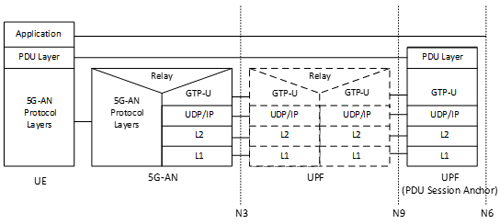
\includegraphics[width=0.8\textwidth]{resources/images/3gpp_5g_data_plane_protocol.png}
	\caption{3GPPP's 5G Data Plane protocol stack \cite{3gpp_5g_system_overview}}
    \label{fig:introduction:3gpp_5g_data_plane_protocol}
\end{figure}


\section{Problem Statement}\index{Requirements}\label{sec:introduction:problem_statement}
% In this section, the problems with single-link tunnel will be presented.
% Combine links
% The most commonly used technologies for communication in data center and \ac{HPC} environment are Ethernet and \ac{infinibandpage} (\Cref{fig:introduction:Interconnect_Technologies_500_supercomp}), which currently offer 100-200Gb/s bandwidth per line \cite{ethernet_roadmap}\cite{infiniband_roadmap}.
% These kind of bandwidth between computers (or inter-system) are nonetheless impressive, yet not comparable to the system's internal connection, i.e inter-chiplet bridge \textit{Infinity Fabric} used in AMD's Zeppelin SoC provides 256GB/s in-package bandwidth \cite{burd_zeppelin_2019}, and up to 800GB/s connection in GPUs peer-to-peer test \cite{amd_infinity_architecture}.
% This means even when invested in the current latest networking hardware, the connection between computer instances might be the bottleneck for certain applications that require distributed computation, for example large \ac{AI} or simulation model.
% In this case, a multipath tunnel can hide hide the multipath details of merging multiple links from the applications, effectively scales up the network capacity horizontally.
% The tunnel thus allow data center usage benefits from having larger combined bandwidth using current technology, but also is a necessary tool to overcome eventual physical and economical limitation in the future.
% For less demanding usages, aggregation is an affordable method to build fast connection from available hardware \todo{improve}.
Ethernet and InfiniBand are the most prevalent communication technologies in data centers and \ac{HPC} environments. 
Currently, these technologies provide bandwidths of 100-200Gb/s per line \cite{ethernet_roadmap}\cite{infiniband_roadmap} (\Cref{fig:introduction:Interconnect_Technologies_500_supercomp}). 
While this bandwidth is impressive for inter-system communication, it cannot match the internal connections within a system. 
For instance, AMD's "Infinity Fabric" bridge offers an in-package bandwidth of 256GB/s on Zeppelin SoC family \cite{burd_zeppelin_2019}, and up to 800GB/s in peer-to-peer tests between GPUs using more bands \cite{amd_infinity_architecture}.
This indicates that even with the latest networking hardware, the connection between computer instances can become a bottleneck for distributed data-intensive applications, for instance large \ac{AI} model or computer simulation. 
In such cases, a multipath tunnel can abstract the complexity of merging multiple links from the applications, effectively scaling up the network capacity horizontally. 
Consequently, the multipath tunnel enables data centers to benefit from larger combined bandwidth using current technology and serves as a necessary tool to overcome future physical and economic limitations.
For less demanding use cases, aggregation presents an affordable method to build fast connections using available hardware.
%
% Reliability
% Connection's reliability is closely related to the failure probabilities of the individual links and nodes (component reliability, can directly effect service availability) \cite{shooman_algorithms_1995} and the \ac{QoS} parameters \cite{gozdecki_quality_2003}.
% Common connection's \ac{QoS}  parameters can be named: latency, peak throughput, jitter.
% Depends on the use case, reliability of the connection can be a \ac{QoS} measurement factor (i.e commercial network provider) or a strict requirement (i.e critical application).
% Generally, 2 non-exclusive strategies are often used to increase a connection's reliability: through fortifying individual link, or redundancy.
% A connection's failure probability can be reduced by upgrading to a more resilient but expensive link or equipping with multiple failover lines. 
% Similarly, while better hardware can eliminate many \ac{QoS} inadequacy problems, having multiple links (or routes) each optimized for a type of appliance is certainly more suitable and affordable for the operator, especially if the data traffic is heterogeneous \cite{chen_overview_1998}.
% A multipath tunnel with flow-aware capability can be used in this case to manage the underlying links as an abstraction layer for the applications that utilize the connection. \todo{improve} \todo{more about QoS}
The reliability of a connection is closely tied to the failure probabilities of the individual links and nodes, which directly impacts service availability \cite{shooman_algorithms_1995}. 
Additionally, \ac{QoS} parameters such as latency, peak throughput, and jitter play a crucial role \cite{gozdecki_quality_2003}.
Depending on the use case, connection reliability can either serve as a \ac{QoS} measurement factor (e.g., for commercial network providers) or a strict requirement (e.g., for critical applications). 
Generally, there are two non-exclusive strategies commonly employed to enhance connection reliability: strengthening individual links or incorporating redundancy.
% Upgrading to more resilient, albeit costly, hardware links or implementing multiple failover lines can reduce the probability of connection failures. 
While superior hardware can reduce the probability of connection failures and address many \ac{QoS} inadequacies, having multiple links or routes optimized for specific applications is often a more practical and cost-effective approach for operators, particularly when dealing with heterogeneous data traffic \cite{chen_overview_1998}.
In such cases, a multipath tunnel with flow-aware capabilities can be utilized as an abstraction layer to manage the underlying links for applications relying on the connection. 
This allows for improved reliability and more effective utilization of resources. 
\todo{improve} \todo{more about QoS}

%  heterogeneous data traffic

%%
% Combine with a powerful CPU, networking application based on technologies such as \ac{dpdkpage} can saturate even a 100Gbit line using a single CPU core \cite{intel_dpdk_perf}. 
% However, this can be improved by combining bandwidth of many links. 
% A multipath tunnel will create a logical NIC for application, effectively abstracts the management, orchesteration tasks for the applications.
% \todo{sota: how these are being done in real life?}
% Such method can be useful for long term and short term usage: using existing technology and hardware to achieve higher bandwidth to reduce cost, and overcome physical limitation.

\begin{figure}[H]
	\centering
	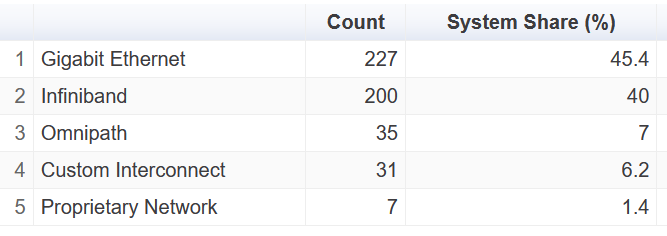
\includegraphics[width=0.8\textwidth]{resources/images/Interconnect_Technologies_500_supercomp.PNG}
	\caption{Interconnect technologies of top 500 super computers, 2023 edition as tracked by TOP500 project \cite{Interconnect_Technologies_500_supercomp}}
    \label{fig:introduction:Interconnect_Technologies_500_supercomp}
\end{figure}

\todo{other: latency, ...}

% Perf: userspace vs kernelspace process
% Omitting trivial tasks such as authentication and handshake, tunneling operation including the following steps: acquiration of ingress data stream (send to tunnel by application), process of ingress data (convert data into stream of tunnel packets, often through encapsulating with tunnel header, encrypting, compressing), and reverse on the receiving end (extrating original data from tunnel packets and delivering to application) \todo{cite+improve}.
% Apart from scaling the underlying system vertically (i.e by using more powerful hardware) or using a lower-level programing language, the most significant factor that could affect the performance of a single-link tunnel implementation is how ingress data is handled.


% \sidenote{State of the Art}
% \todomid{write about the State of the Art}

% \sidenote{Issue:\\Example 1}
% \todomid{write about the first issue}

% \sidenote{Issue:\\Example 2}
% \todomid{write about the second issue}

% \sidenote{Synopsis}
% \todomid{write about the synopsis of the issues and \Cref{fig:intro:c}}

% \begin{figure}[htbp]
%     \centering
%     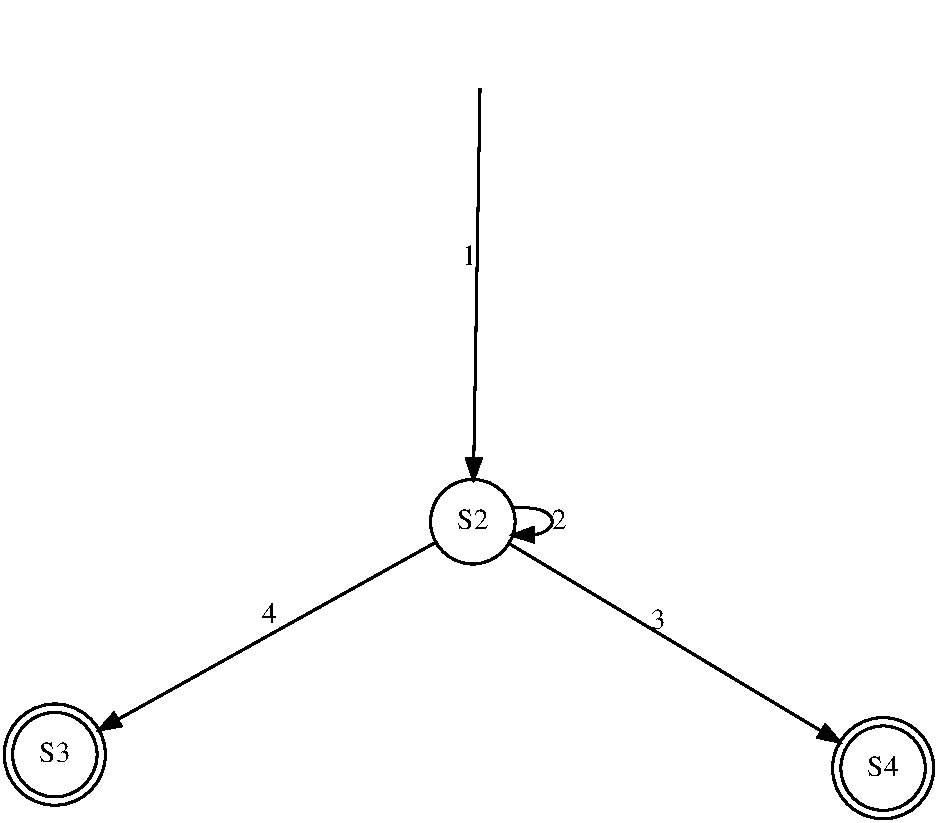
\includegraphics[width=.5\textwidth]{resources/images/job_lifecycle}
%     \caption{Relationship between issues}\label{fig:intro:c}
% \end{figure}

\section{Assumptions and Scope}

% \sidenote{Research Assumptions}
% \todomid{write about the research assumptions~\cite{li2002design}}
Besides the reliability's \ac{QoS} characteristic, we define the metrics to measure performance of a tunnel as follow:
\begin{itemize}
    \item Bandwidth: Quantity of data that can be transmitted through per second, usually measured in Megabit per Second (Mb/s) or Gigabit  per Second (Gb/s)
    \item Latency: Delay, measured in microsecond (us) or millisecond (ms). Latency introduced by the tunneling process at both ends compared to sending data over the same public path without the tunnel.
    \item System load: Tunneling process costs CPU time and RAM usage.
\end{itemize}

% The idea
The project is inspired by \ac{5G}'s \ac{NFV} and \ac{SDN} influenced specification.
Being recognized as the 2 technology enabler for realizing 5G networks, they allow concepts such as \textit{slicing} or \textit{decoupling} of hardware-software planes and control-data planes \cite{yousaf_nfv_sdn_key_techno_for_5g2017} \cite{open_baton} which make \ac{5G} a much more capable network standard than its predecessor while remains flexible and agile for operators \todo{better wording here}.
\ac{NFV} moves dedicated functions such as router, firewall that traditionally ran on dedicated hardware to virtualized environment and cloud-based infrastructure.
\ac{SDN} encourages using software based solution running on common hardware and software stack over conventional equipment and services which integrated on rigid hardware-based proprietary.
\ac{NFV} and \ac{SDN} thus helps reducing capital and operational expenditures, speeding up the release process and avoid vendor locking \cite{yousaf_nfv_sdn_key_techno_for_5g2017} \cite{sun_integrating_2015}.
These trends heavily influence the 5G infrastructure to employ recent software industry's practices, which include agile development, orchestration, moving to cloud, dynamic deployment, and \ac{HA} through horizontal partition.
\ac{5G}'s distributed network services and diverse \ac{QoS} require reliable and high throughput connection, which as discussed in \Cref{sec:introduction:problem_statement} can be horizontally implemented in an performant and cost-effective way using multiple links instead of vertical scaling paradigm.

% building block:
Moving functions to cloud and virtual environment faces performance challenges, one of which is the overhead introduced by the abstraction, virtualization layers as well as the extra input/output and communication between functions that can be found locally before \cite{yousaf_nfv_sdn_key_techno_for_5g2017}.
Although the running newly designed cloud-native software on orchestrated thin containers help addressing the performance problem, we believe some aspects of the connection can be improved further, namely compatibility and ease of development and deployment.
In many 5G's implementation, technologies such as \ac{dpdkpage} and \ac{sriov} are being used to deliver line-speed packet processing capability to hypervisor environment with minimal impact on system performance \cite{intel_dpdk_perf} \cite{openstack_sriov} \cite{zte_5g_core_upf_impl} \cite{nec_hite_paper_upf_perf}.
We believe that these technologies proved their worthy, yet the systems suffer from limitation such as special requirement and configuration \todo{cite, that dpdk and sriov can't run on all commercial system}.
This would not only increase cost, but also make the product less attractive for research and test bed purposes, especially in the open source and academy community where budget and custom support is limited.
To address this, using a native and more simple Linux's technology - \ac{xdppage}, a new socket family based on eBPF technology with comparable performance to \ac{dpdkpage} - to build a tunnel that is designed to support multipath and multi-flow could be a promising supplement for existing implementation. \todo{more}


% \sidenote{Research Scope}
% \todomid{write about the research scope --- \Cref{fig:intro:a,fig:intro:b,fig:intro:c}}
With an implementation and a thesis documentation for the multipath tunnel as the desire outcome of the project , we define the scope of the project as followed:
\begin{itemize}
    \item Scope of research: this research is limited to investigating a tunnel implementation based on \ac{xdppage} technology that employs multipath and flow-aware concepts. A functional tunnel is expected to be built in 3 months. From there, more complex features will be added along with a test application to run on top the tunnel for testing and demonstrating purposes. In the course of building process, this initiated documentation will be updated until the project reaches its time limitation (6 months in total). Although the tunnel library will be a general purpose framework that can be deployed for any application, it is intended to be tested with 5G's software stack in mind.
    \item Foreseeable tasks: researching the project idea, building multipath protocol, implementing the tunnel, testing and demonstrating tasks are planed. 
    \item Implementation: the tunnel will be implemented in C/C++, uses \ac{xdppage} sockets as the packet transport layer. The tunnel shall be able to exchange data over multiple \ac{NIC}s and treat each packet differently based on defined configuration (stream based/flow based). More will be discussed in the next section.
    \item Demonstration: used to test and present the features of the tunnel. At this stage, a simplified version of \ac{gptu} protocol has been chosen to run on top of the tunnel. \ac{gptu} is the communication protocol responsible for establishing data exchanging channels in 5G's \ac{UPF} and gNodeB. These channels (or tunnels) handle streams of data, each has \ac{QoS} identifier with different characteristics and priority. This makes the protocol a good match for tunnel demonstration purpose.
\end{itemize}


\section{Objectives and Contributions}
The research is limited to investigating the multipath concept with a new technology. 
Generally, the tunnel implementation can be useful for the following scenarios:
\begin{itemize}
    \item High bandwidth connection for High performance computing, servers, data center.
    \item High reliability for critical application by using backup links for tunnel or replicate packets.
    \item 5G back-haul and middle-haul: power the forwarding/relaying mechanism (\ac{UPF}, gNodeB's UD-CU). Enhance existing GTP-U protocol with multipath, flow-aware capability.
\end{itemize}

Although we hope the project's outcome can contribute to the general understanding of software based solution for high performance networking field, we seek opportunity to integrate the tunnel into the next generation telecommunication system. We found 2 potential improvements according to our research: \todo{improve the following text}
\begin{itemize}
    \item N6 connection between UPF (also N9 i.e between UPF-E and UPF-C) and Data network: enhanced by prioritized, flow-aware, high bandwidth multipath tunnel. To meet differentiated SLA requirements for latency, bandwidth and reliability, UPF needs to be deployed at different positions including central DC, regional DC, edge DC and campus DC. MTX can help saturating physical links coup with support large number of UEs.
    \item 5G user plane (back-haul N3 between gNodeB-UPF, mid-haul between gNodeB-CU and -DU) relied on message-based protocol \ac{gptu} (the character "U" means "user data tunneling") to relay traffic in tunnels - or flows within a PDP session.
\end{itemize}

We also identified reports regarding performance issues in the \ac{UPF} of \ac{o5gs} - a well-known 5G core implementation that the AV team at the TU Berlin is currently using in their 5G test bed. Contributors have proposed employing \ac{dpdkpage} and exploring lower-level approaches to minimize overhead \cite{open5gs_github_dpdk}\cite{open5gs_github_udp_perf_cap}, as the current implementation limits the TUN interface bandwidth to 1Gbit. We believe that through thorough analysis, this presents an opportunity for us to make a valuable contribution to the \ac{o5gs} project with our MTX tunnel.

\begin{figure}[H]
	\centering
	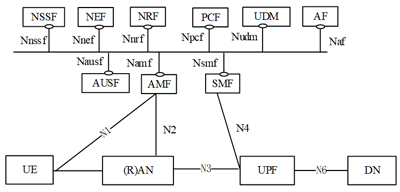
\includegraphics[width=0.8\textwidth]{resources/images/3gpp_5g_system_overview.png}
	\caption{3GPP's 5G System Overview \cite{3gpp_5g_system_overview}}
    \label{fig:introduction:3gpp_5g_system_overview}
\end{figure}


% \begin{figure}[htbp]
%     \centering
%     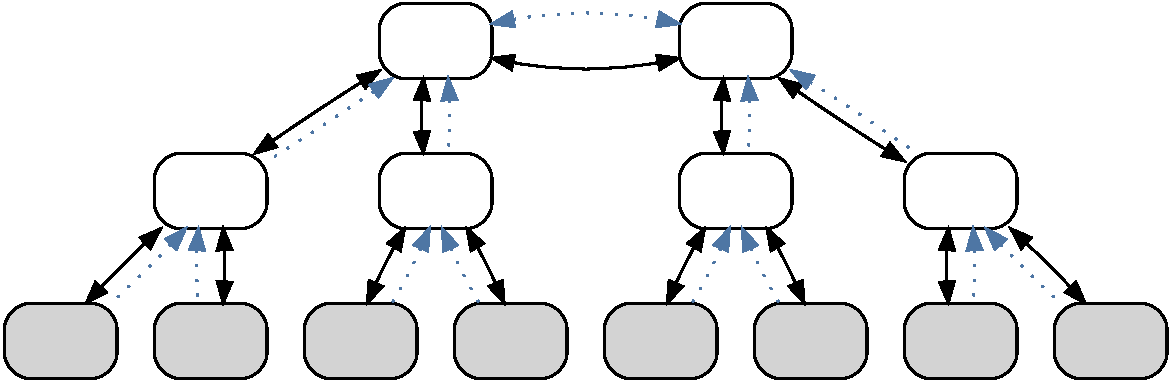
\includegraphics[width=.55\textwidth]{resources/images/example3}
%     \caption{Structure of research}\label{fig:intro:struct}
% \end{figure}

% \sidenote{Research Objectives \& Contributions}
% \todomid{write about the research objectives and \ac{DBpedia} and \Cref{fig:intro:struct}}

% \section{Methodology and Outline}

% \todomid{write about the research outline and \Cref{fig:intro:methodology}. Summarize \Cref{sec:introduction,sec:sota,sec:reqs,sec:contrib1,sec:contrib2,sec:contrib3,sec:eval,sec:summary}.}

% \begin{sidewaysfigure}
%     \centering
%     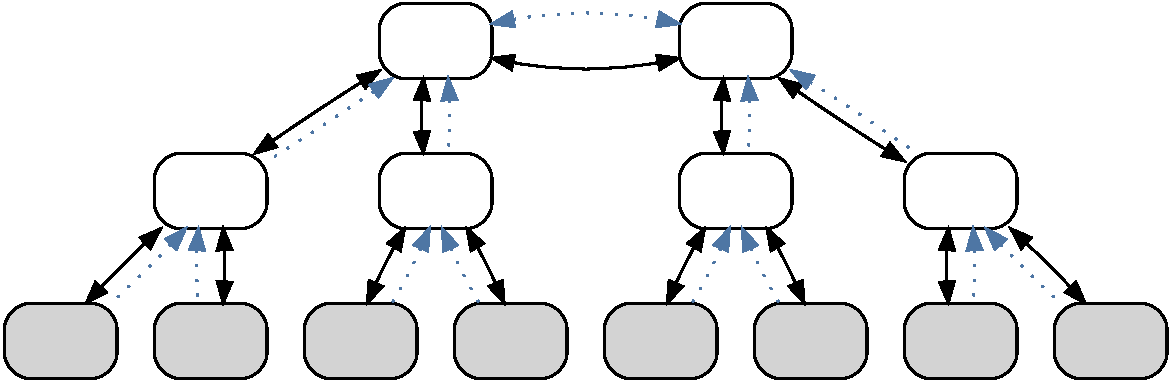
\includegraphics[width=.7\textwidth]{resources/images/example3}
%     \caption{Workflow of the research and structure of the thesis}\label{fig:intro:methodology}
% \end{sidewaysfigure}

    % \cleardoublepage\chapter{State of the Art}\label{sec:sota}\minitoc\vspace{.5cm}\index{SotA}
This chapter provides a comprehensive and technical explanation of the aforementioned technologies mentioned earlier. 
The detail of DPDK and SR-IOV and their usage in current 5G system will be introduced in more detail.
Subsequently, the chapter presents the fundamental concept and design of eBPF and AF\_XDP, which is crucial for the implementation of the MTX library.

\section{DPDK: Data Plane Development Kit}
\ac{dpdkpage} is a library initially developed by Intel engineer Venky Venkatesan and currently maintained by the Linux Foundation. 
It provides a solution that contains a collection of libraries, poll drivers and configuration designed to accelerate packet processing workloads. 
By decoupling the NIC and CPU cores from the kernel, the library establishes a highly efficient and high-throughput data path, thus eliminates the overhead introduced by Linux kernel's network stack \cite{kourtis_enhancing_2015}. 
\ac{dpdkpage} has been widely utilized in various projects, including pfSense, Open vSwitch/OpenStack, Intel's DDP, OpenFlow, and 5G UPF implementations \cite{intel_ddp_ethernet_800}\cite{pongracz_removing_2013}\cite{zte_5g_core_upf_impl}\cite{nec_upf_whitepaper}. 
\\

From a technical standpoint, \ac{dpdkpage} is a complex kernel-bypassing library to process network packets that can deliver packets to application in user space with very low latency.
In addition, \ac{dpdkpage} offers a range of powerful features, including Crypto, DMA direct memory access, CUDA GPU utilization, and Machine Learning Device Driver \cite{dpdk_guide_page}. 
\ac{dpdkpage} is however, not a networking stack and has no Layer-3 forward, IPsec, firewall features \cite{old_dpdk_page}, thus forces developers to maintain their own code base for such purposes.
Therefore, using \ac{dpdkpage} in small open-source projects may necessitate more extensive maintenance and configuration compared to utilizing an in-kernel alternative like \ac{xdppage} socket, which will be utilized to construct our MTX library.
Unlike \ac{dpdkpage}, \ac{xdppage} socket has no monopoly on the \ac{NIC}, thus allows the kernel to manage and share the hardware resource to other applications.

\section{SR-IOV: Single Root I/O Virtualization}
\begin{figure}[H]
	\centering
	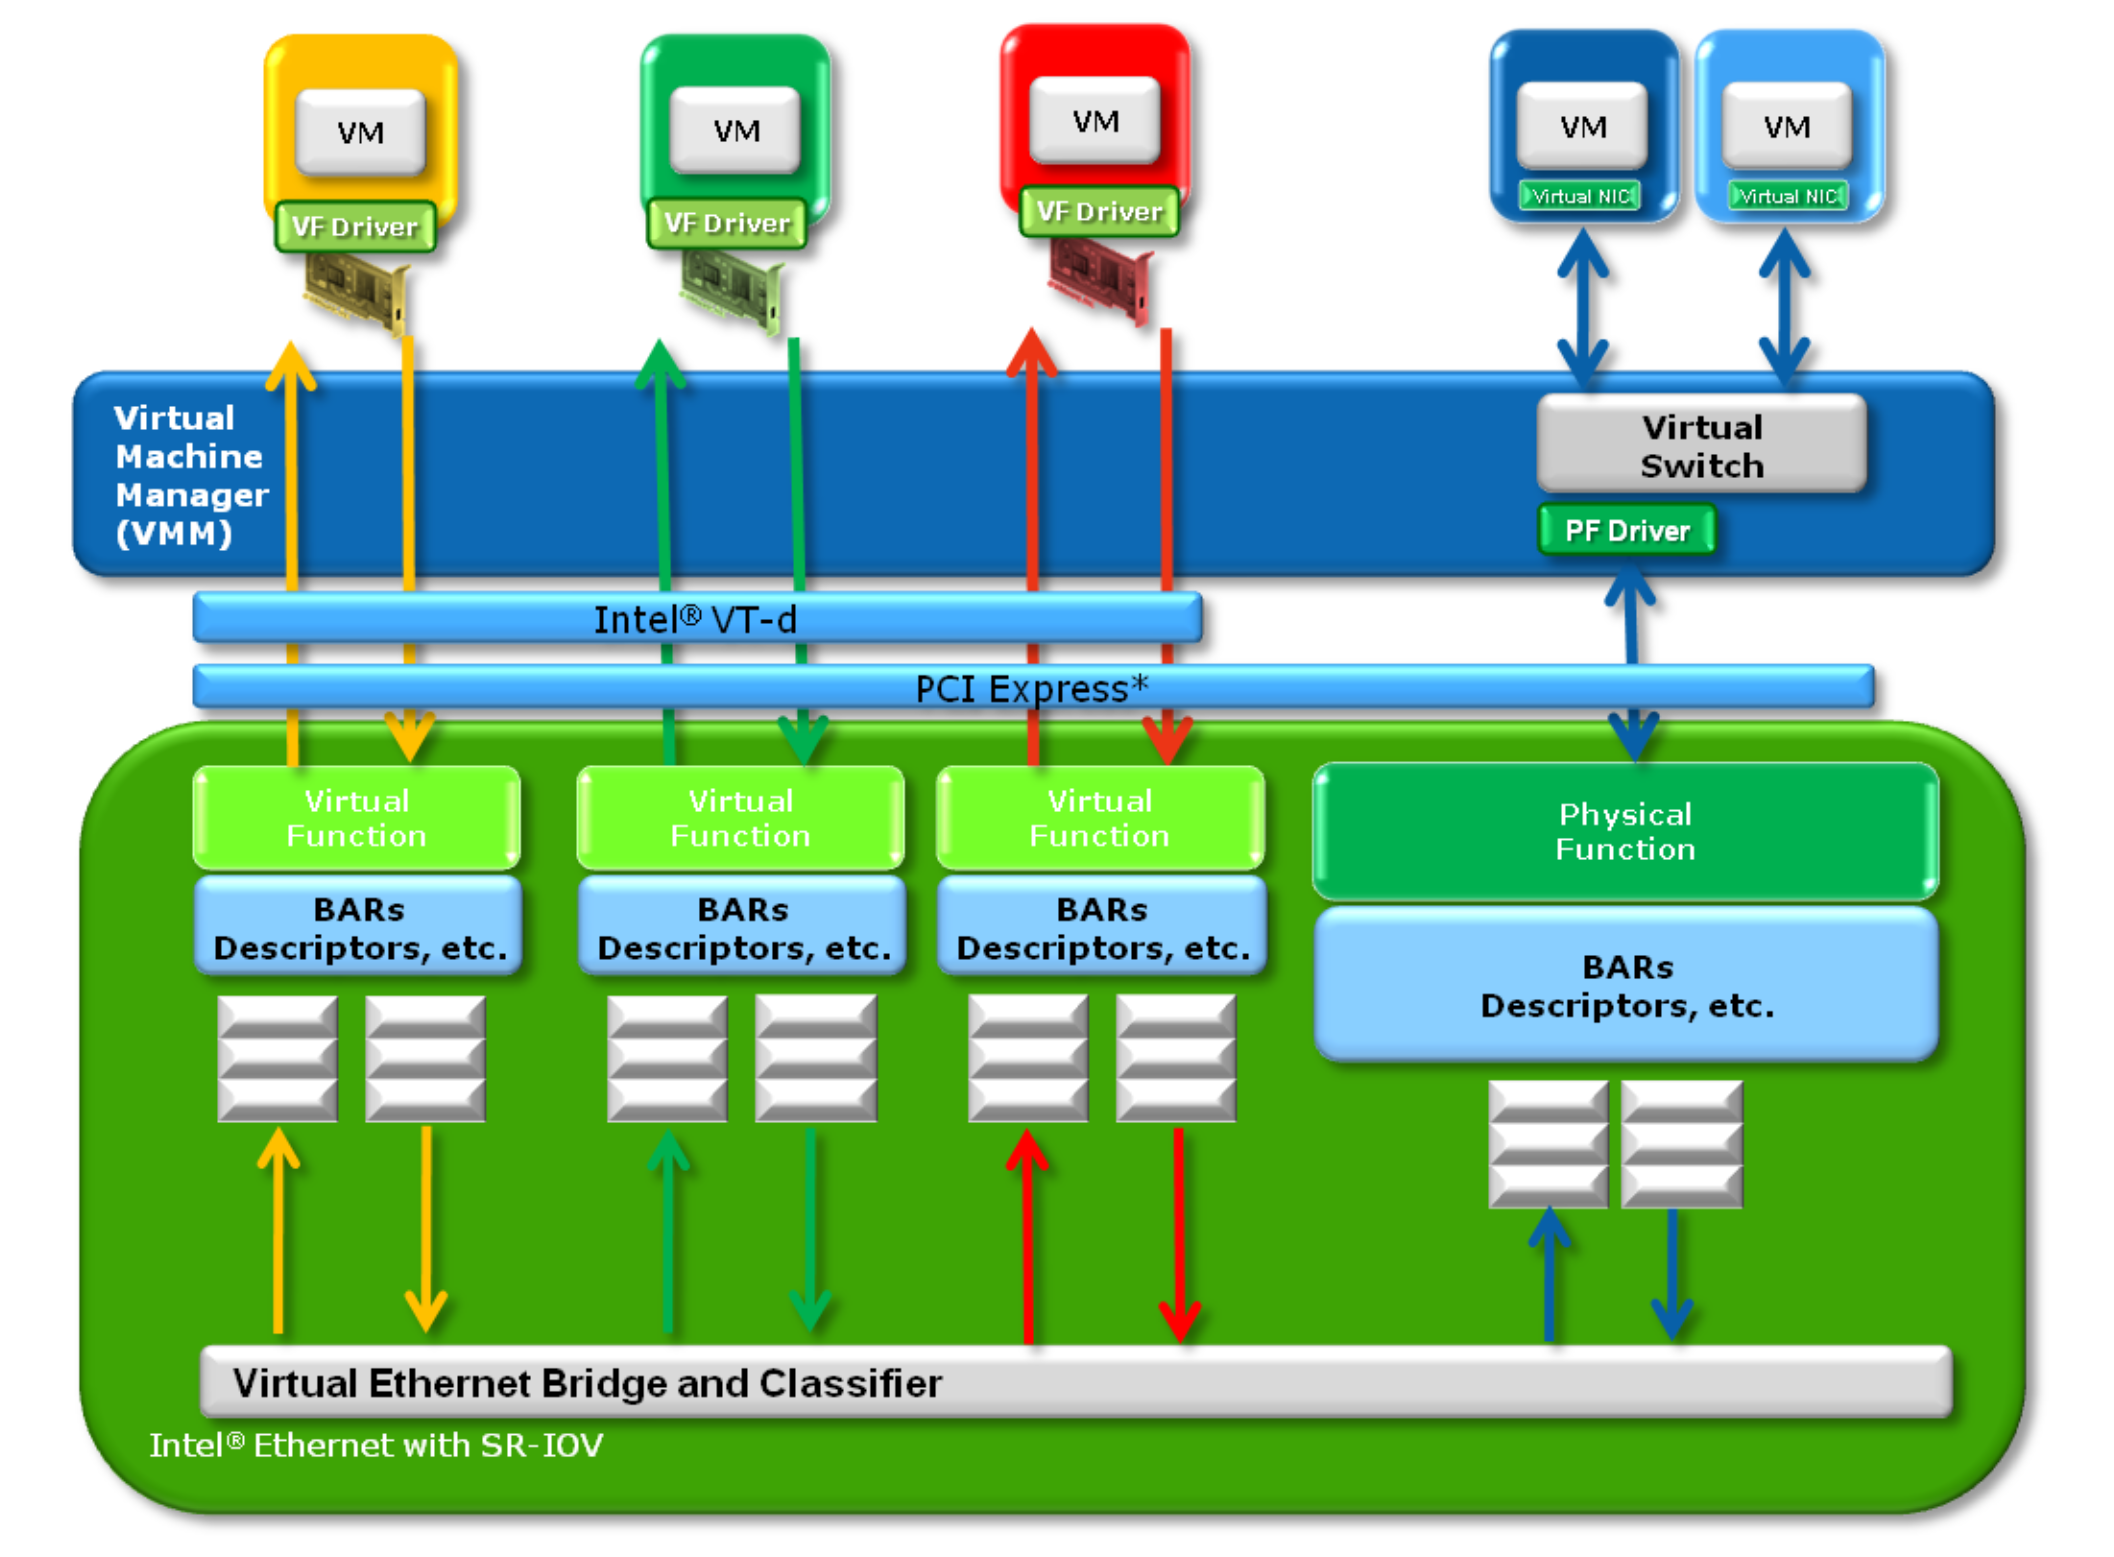
\includegraphics[width=1.0\textwidth]{resources/images/intel_sriov_Natively_and_Software_Shared.PNG}
	\caption{Natively (3 virtual machines on the left) and Software Shared \cite{intel_sriov}. The function type \textit{Virtual Function} (VF) can access a limited set of Base Address Register (BAR) descriptors (which holds the address of mapped memory of the device, or so called configuration space) and other parameters compared to the type \textit{Physical Function}. VF is designed to provide only the resources necessary for data movement.}
    \label{fig:sota:intel_sriov_Natively_and_Software_Shared}
\end{figure}

\ac{sriov} is a \ac{PCIe} specification that allows a physical \ac{PCIe} device to be partitioned into logical devices which appear as multiple physical devices in the guest \ac{OS} \cite{ibm_sriov}\cite{vmware_sriov}. 
By providing independent memory space, interrupts, and \ac{DMA} streams for each virtual machine, the natively shared devices achieve low latency and lower CPU utilization compared to virtual devices provided by traditional \ac{VMM}'s Virtual Switch or  I/O emulation layer (see \Cref{fig:related_work:intel_sriov_Natively_and_Software_Shared}) \cite{intel_sriov}.
As the \ac{sriov} specification is developed by \ac{PCISIGfootnote}, the consortium responsible for the \ac{PCIe} standard, there is no risk of vendor lock-in or significantly hidden cost.
A similar but less sophisticated method - namely \ac{PCIe} passthrough - to eliminates emulation overhead on I/O operation in hypervisor environment is completely disconnecting the \ac{PCIe} device from the host kernel and connecting it to the guest \ac{OS} instead, although this makes device sharing impossible.
It is also important to note that the \ac{sriov} specification is specifically designed for passing resources to and from a hypervisor environment, which is not conflict with our intended scenario.
The \ac{MTX} is designed as a general-purpose multipath tunnel that functions on \ac{NIC}s, making \ac{sriov} technology the underlying infrastructure layer for enabling \ac{MTX}'s \ac{xdppage} sockets to operate on the native shared devices.
This is similar to how \ac{ZTE} used \ac{sriov} in conjunction with \ac{dpdkpage} in their software stack \cite{zte_upf_full_whitepaper}.
\\

The Data plane relies on \ac{gptu} protocol with \ac{UDP} as the transport protocol to deliver high volume of data between \ac{UE} and \ac{DN} (see \Cref{fig:introduction:3gpp_5g_data_plane_protocol}), which require powerful processing power and high capable network link.
According to \ac{3GPP}, an non-exhausted list of \ac{UPF}'s responsibility is \textit{packet routing \& forwarding}, packet \textit{inspection}, \textit{buffering}, \textit{sending} and \textit{forwarding} \cite{3gpp_5g_system_architect_spec_release_18}.
In order to meet the \ac{SLA} and \ac{QoS} requirements, the \ac{UPF} needs to be deployed in various locations, such as the edge (edge and campus), regional sites, and central data centers. 
The size and form of each \ac{UPF} instance vary significantly depending on factors such as the number and size of downstream and upstream functions it manages and responds to \cite{zte_upf_full_whitepaper}.

\section{Current 5G deployment}
\begin{figure}[H]
    \centering
    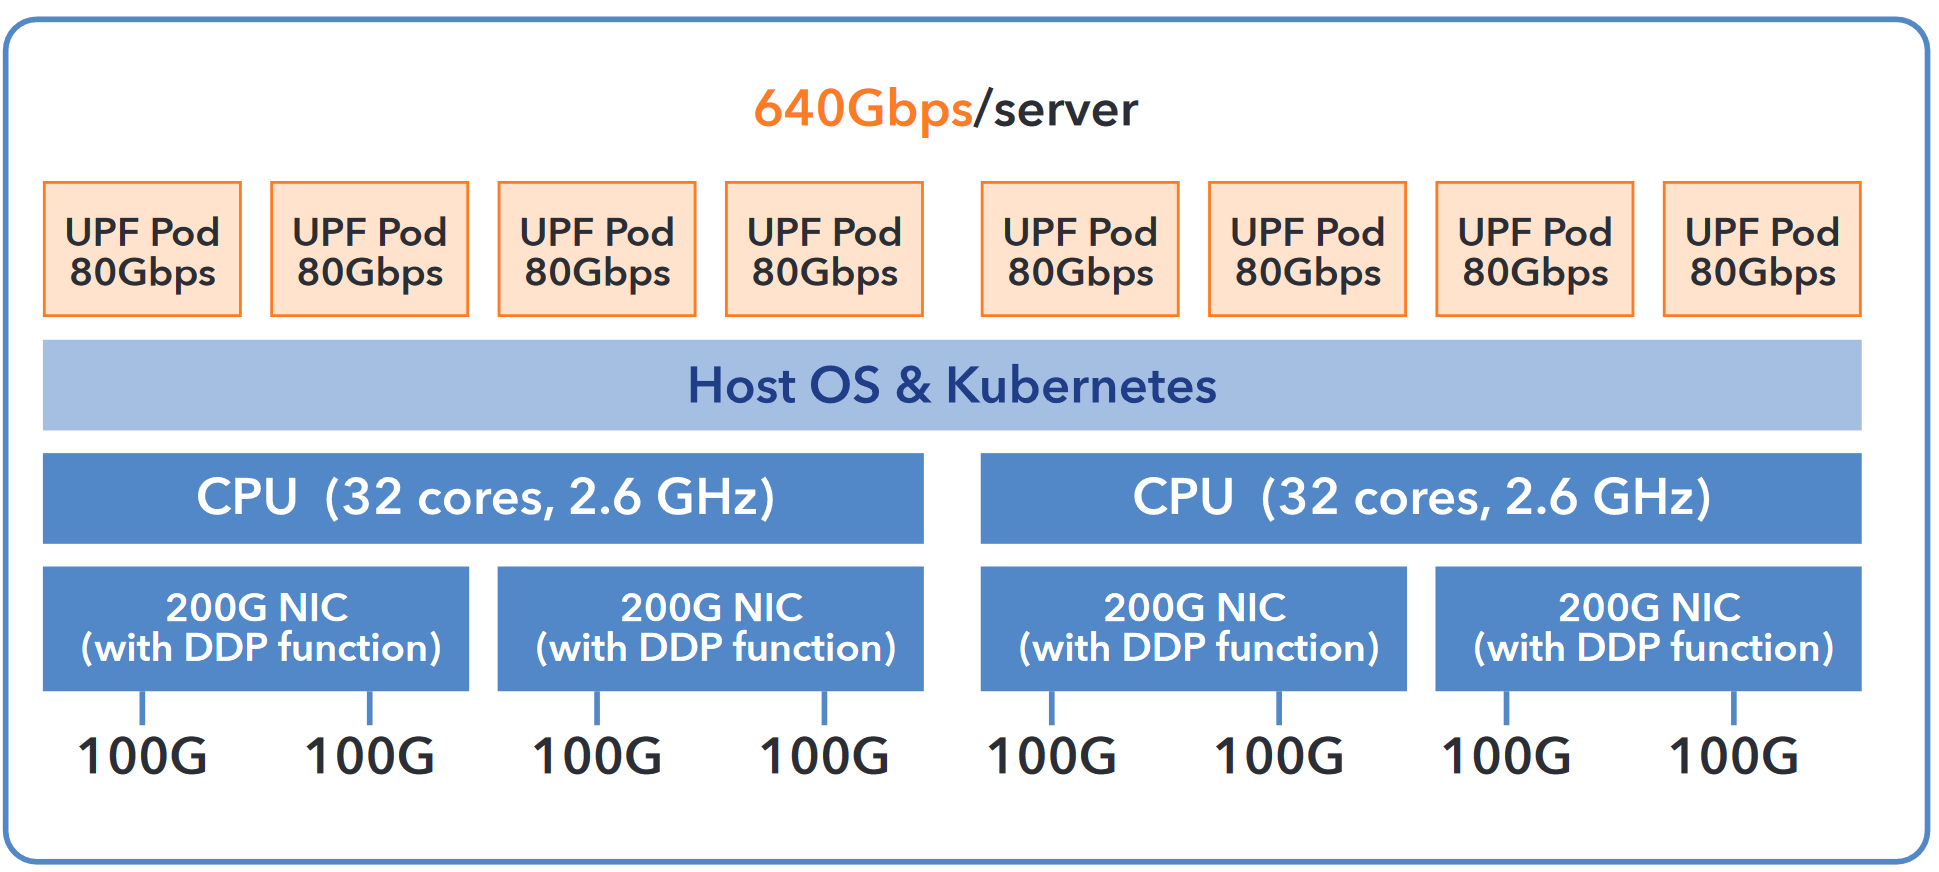
\includegraphics[width=0.6\textwidth]{resources/images/640_nec_upf_system.PNG}
    \caption{NEC's containerized UPF software (8 pods per server) on a platform configured with Linux and Kubernetes \cite{nec_upf_whitepaper}}
    \label{fig:sota:640_nec_upf_system}
\end{figure}
% \begin{figure}[H]
% 	\centering
% 	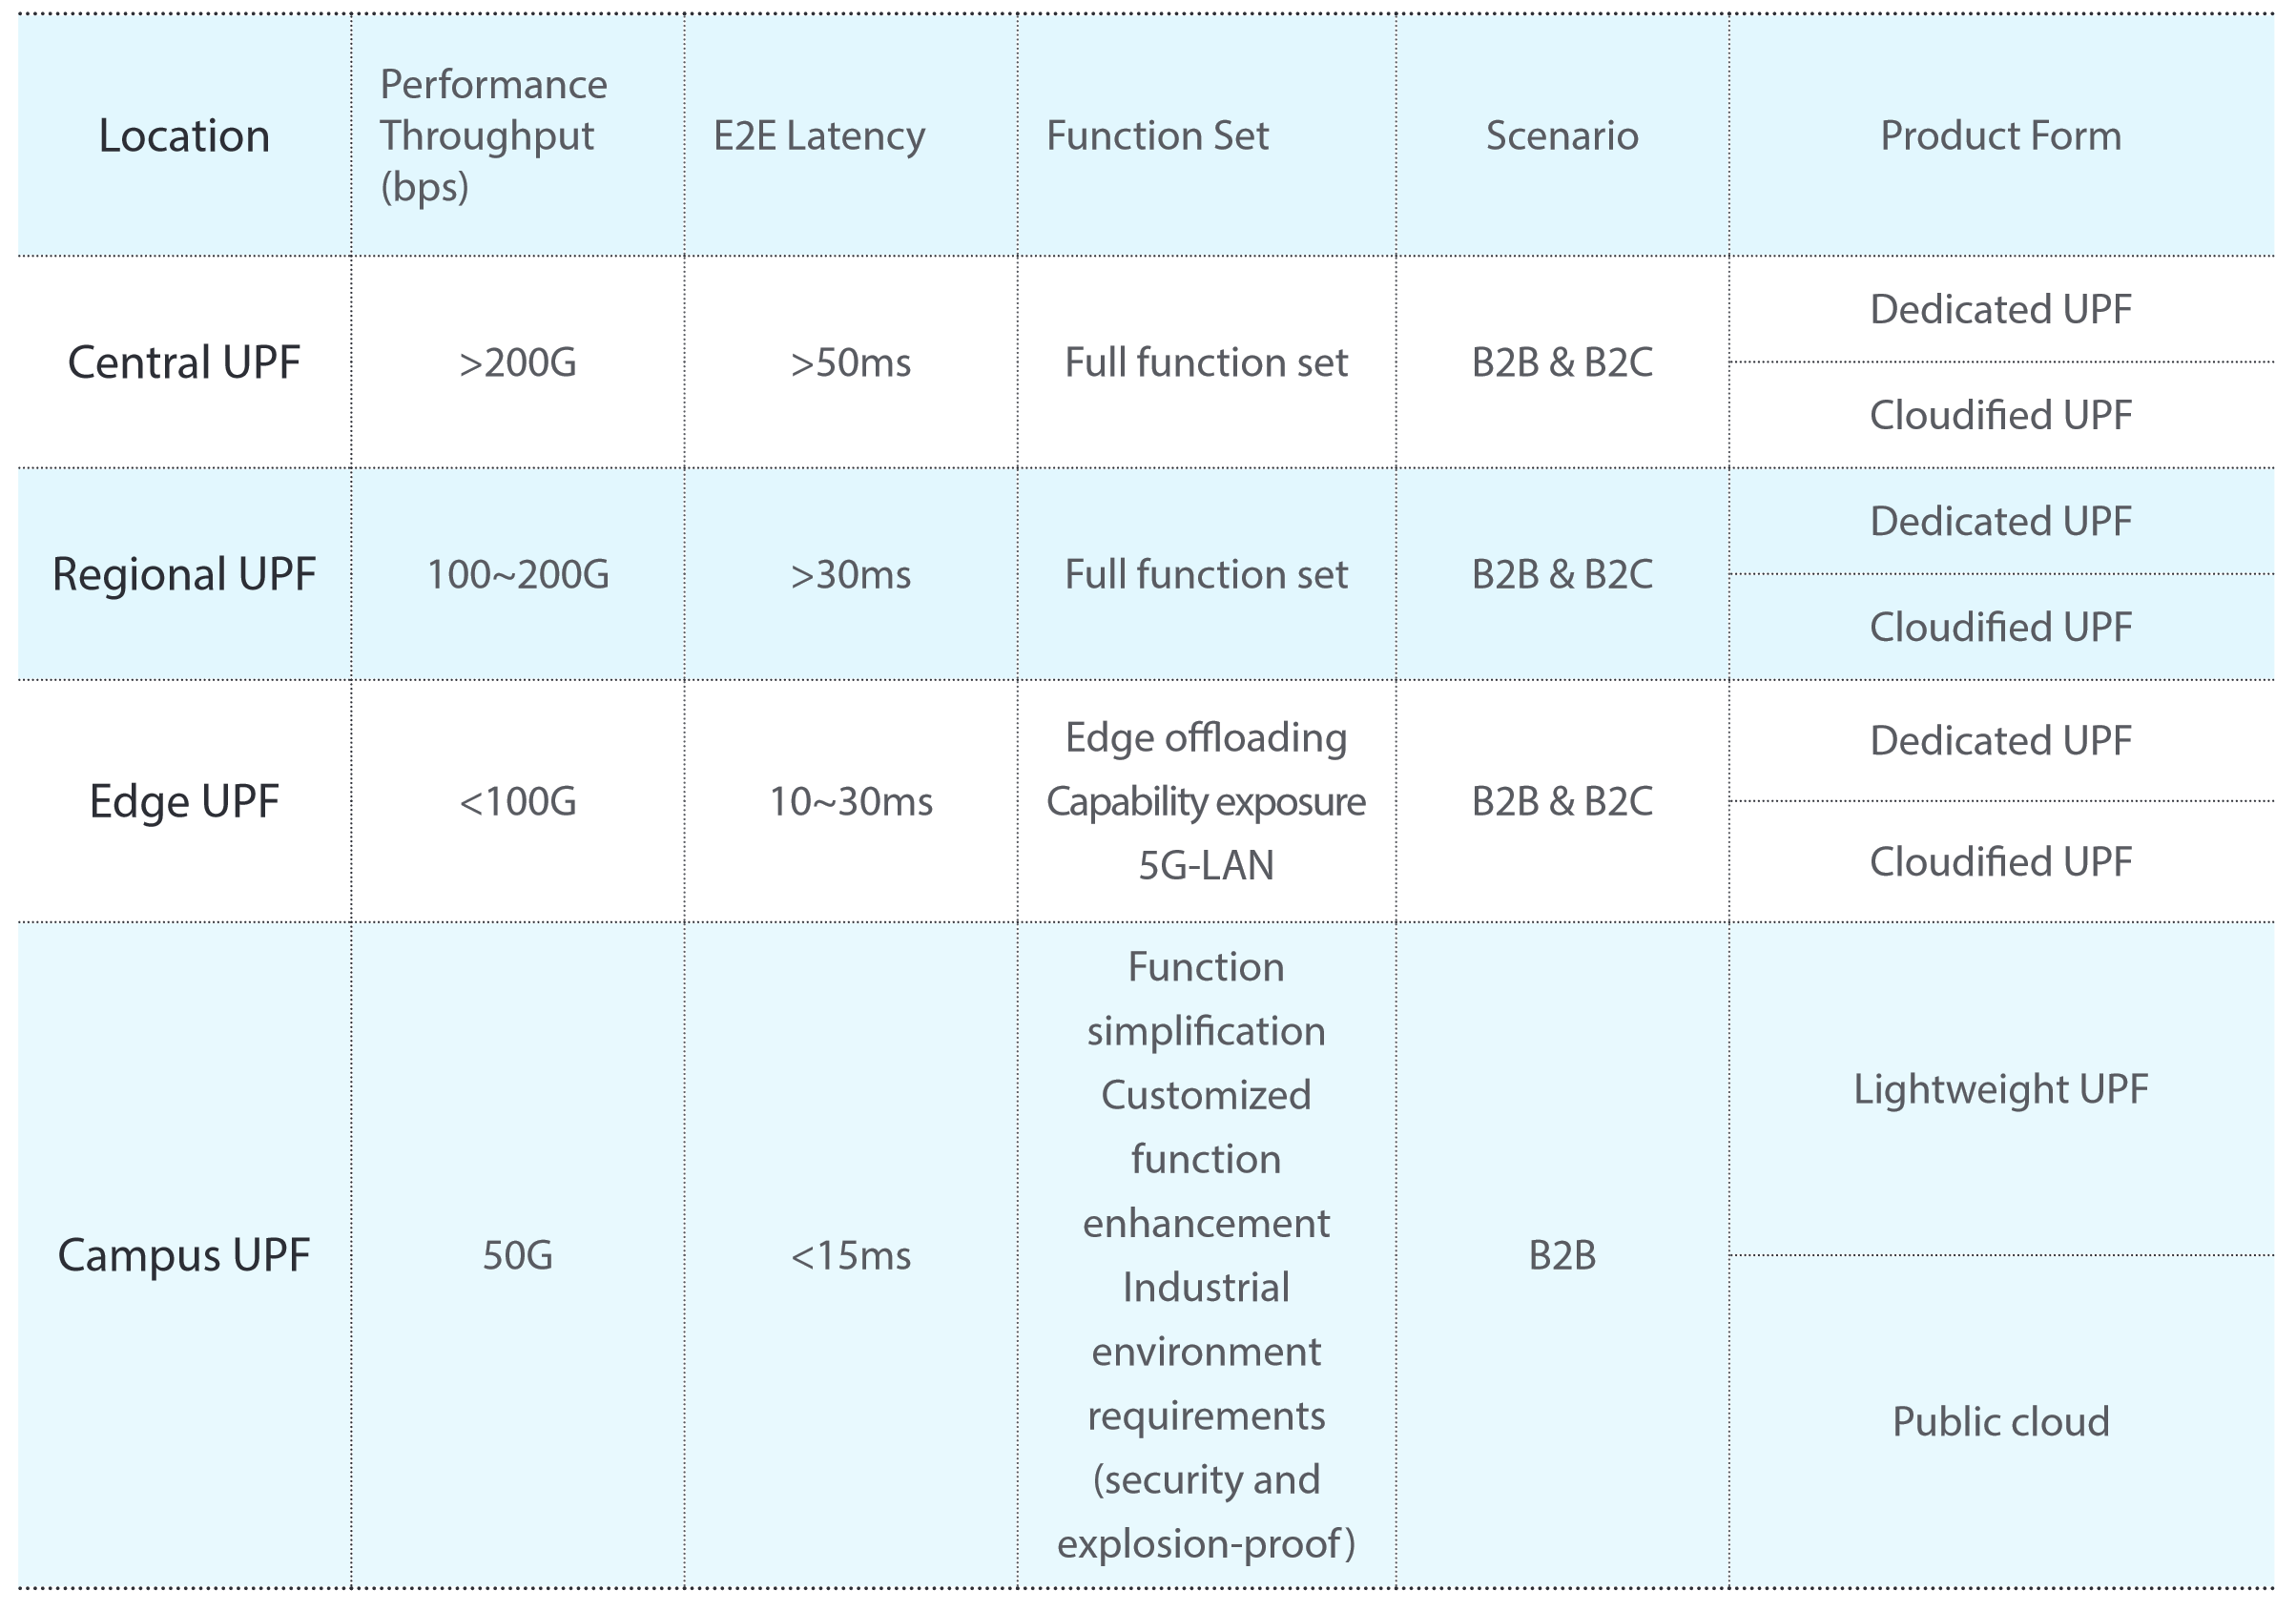
\includegraphics[width=1.0\textwidth]{resources/images/Deployment_Requirements_of_Full_Scenario_UPF.PNG}
% 	\caption{ZTE's White Paper: Deployment Requirements of Full-Scenario UPF \cite{zte_upf_full_whitepaper}}
%     \label{fig:sota:Deployment_Requirements_of_Full_Scenario_UPF}
% \end{figure}

It is common to see 5G services to be implemented and deployed in containers.
The underlying system often manage the containers using an orchestrator, i.e Kubernetes (\Cref{fig:sota:640_nec_upf_system}).

\section{XDP socket: AF\_XDP}
\subsection{Introduction to eBPF and Linux's kernel space}
The kernel functions as the central program of an operating system, overseeing its core operations. 
In a computer system, numerous processes execute concurrently, each fulfilling its assigned tasks. 
However, these processes possess limited access to its surrounding information and are inherently passive.
For instance, a process lacks the ability to initiate or terminate other processes, including itself. 
It operates in a isolated virtual memory and lacks direct communication channels with other processes or devices. 
Furthermore, it lacks awareness of its runtime availability, including when it can execute or must cease, as well as knowledge of its specific memory location, whether in RAM or swap.
Conversely, the kernel assumes the role of a housekeeper, managing the hardware resources of the computer and allocating them among all processes. It facilitates process execution, schedules runtime slots, and mediates communication and events between processes and hardware components.
In addition to these responsibilities, the kernel handles vital tasks such as memory management, providing a file system, establishing networking capabilities, and presenting the system's \ac{API} for programmatic access \cite{kerrisk_linux_2010}.
\\

Linux's virtual memory architecture divides the memory into two distinct spaces: kernel space and user space. This separation provides several advantages, such as enhancing system security and stability \cite{understanding_the_linux_kernel_bovet_cassetti}.
In Linux, tasks can operate in two distinct modes: kernel mode and user mode. When running in user mode, the CPU is restricted from accessing memory allocated for kernel space \cite{kerrisk_linux_2010}.
Invisible to end user, the system switches between kernel mode and user mode very often, usually when a system \ac{API} is involved or a resource needs to be accessed \cite{Robert_linux_kernel_dev}.
Although the CPU supports mode switching, there is a noticeable overhead associated with context switching and memory address translation. 
Running code exclusively in the kernel space has the potential to reduce this overhead and enjoy \textit{better} scheduling policies. 
However, such an approach carries inherent risks, including the possibility of system compromise due to memory leaks, crashes, or malicious exploits \cite{lwn_detect_kernel_mem_leak} \cite{emamdoost_detecting_2021}.
\\

\ac{BPF} technology provides an alternative means of executing code within the kernel space, offering a controlled environment for such operations. 
Initially introduced in 1992 for the \ac{BSD} OS, it was later ported to the Linux platform. 
Originally designed for network packet filtering, \ac{BPF} has since been expanded and utilized for purposes such as firewall management, tracing, and debugging \cite{McCanne_intro_bpf} \cite{lwn_intro_ebpf}. 
Prominent technology companies have leveraged \ac{BPF} for various applications, including: Facebook for firewall, filtering, and load balancing \cite{facebook_katran_ebpf_2018}; Netflix for network monitoring and analysis \cite{netflix_network_insight}; Cilium Project for security and observability purposes \cite{cilium_io_page} and Alibaba for their cloud infrastructure \cite{alibaba_cloud_ebpf}.
\\

\ac{ebpf} - the descendant of \ac{BPF} technology - consisted of a \ac{ebpf} program (also called \textit{kernel program}), the \ac{ebpf} virtual machine provided by the kernel, and the attach code path.
The \ac{ebpf} kernel program is written in a subset of the C programming language and compiled to \ac{ebpf} byte code.
The 64 bit \ac{RISC}-based \ac{ebpf} virtual machine along with a verifier check the code safety and isolate the execution of the \ac{ebpf} kernel program.
To get started, the kernel program is inserted to the desired code path in the kernel where it will be executed whenever the code path is traversed \cite{lwn_intro_ebpf}.

% \begin{figure}[H]
%     \centering
%     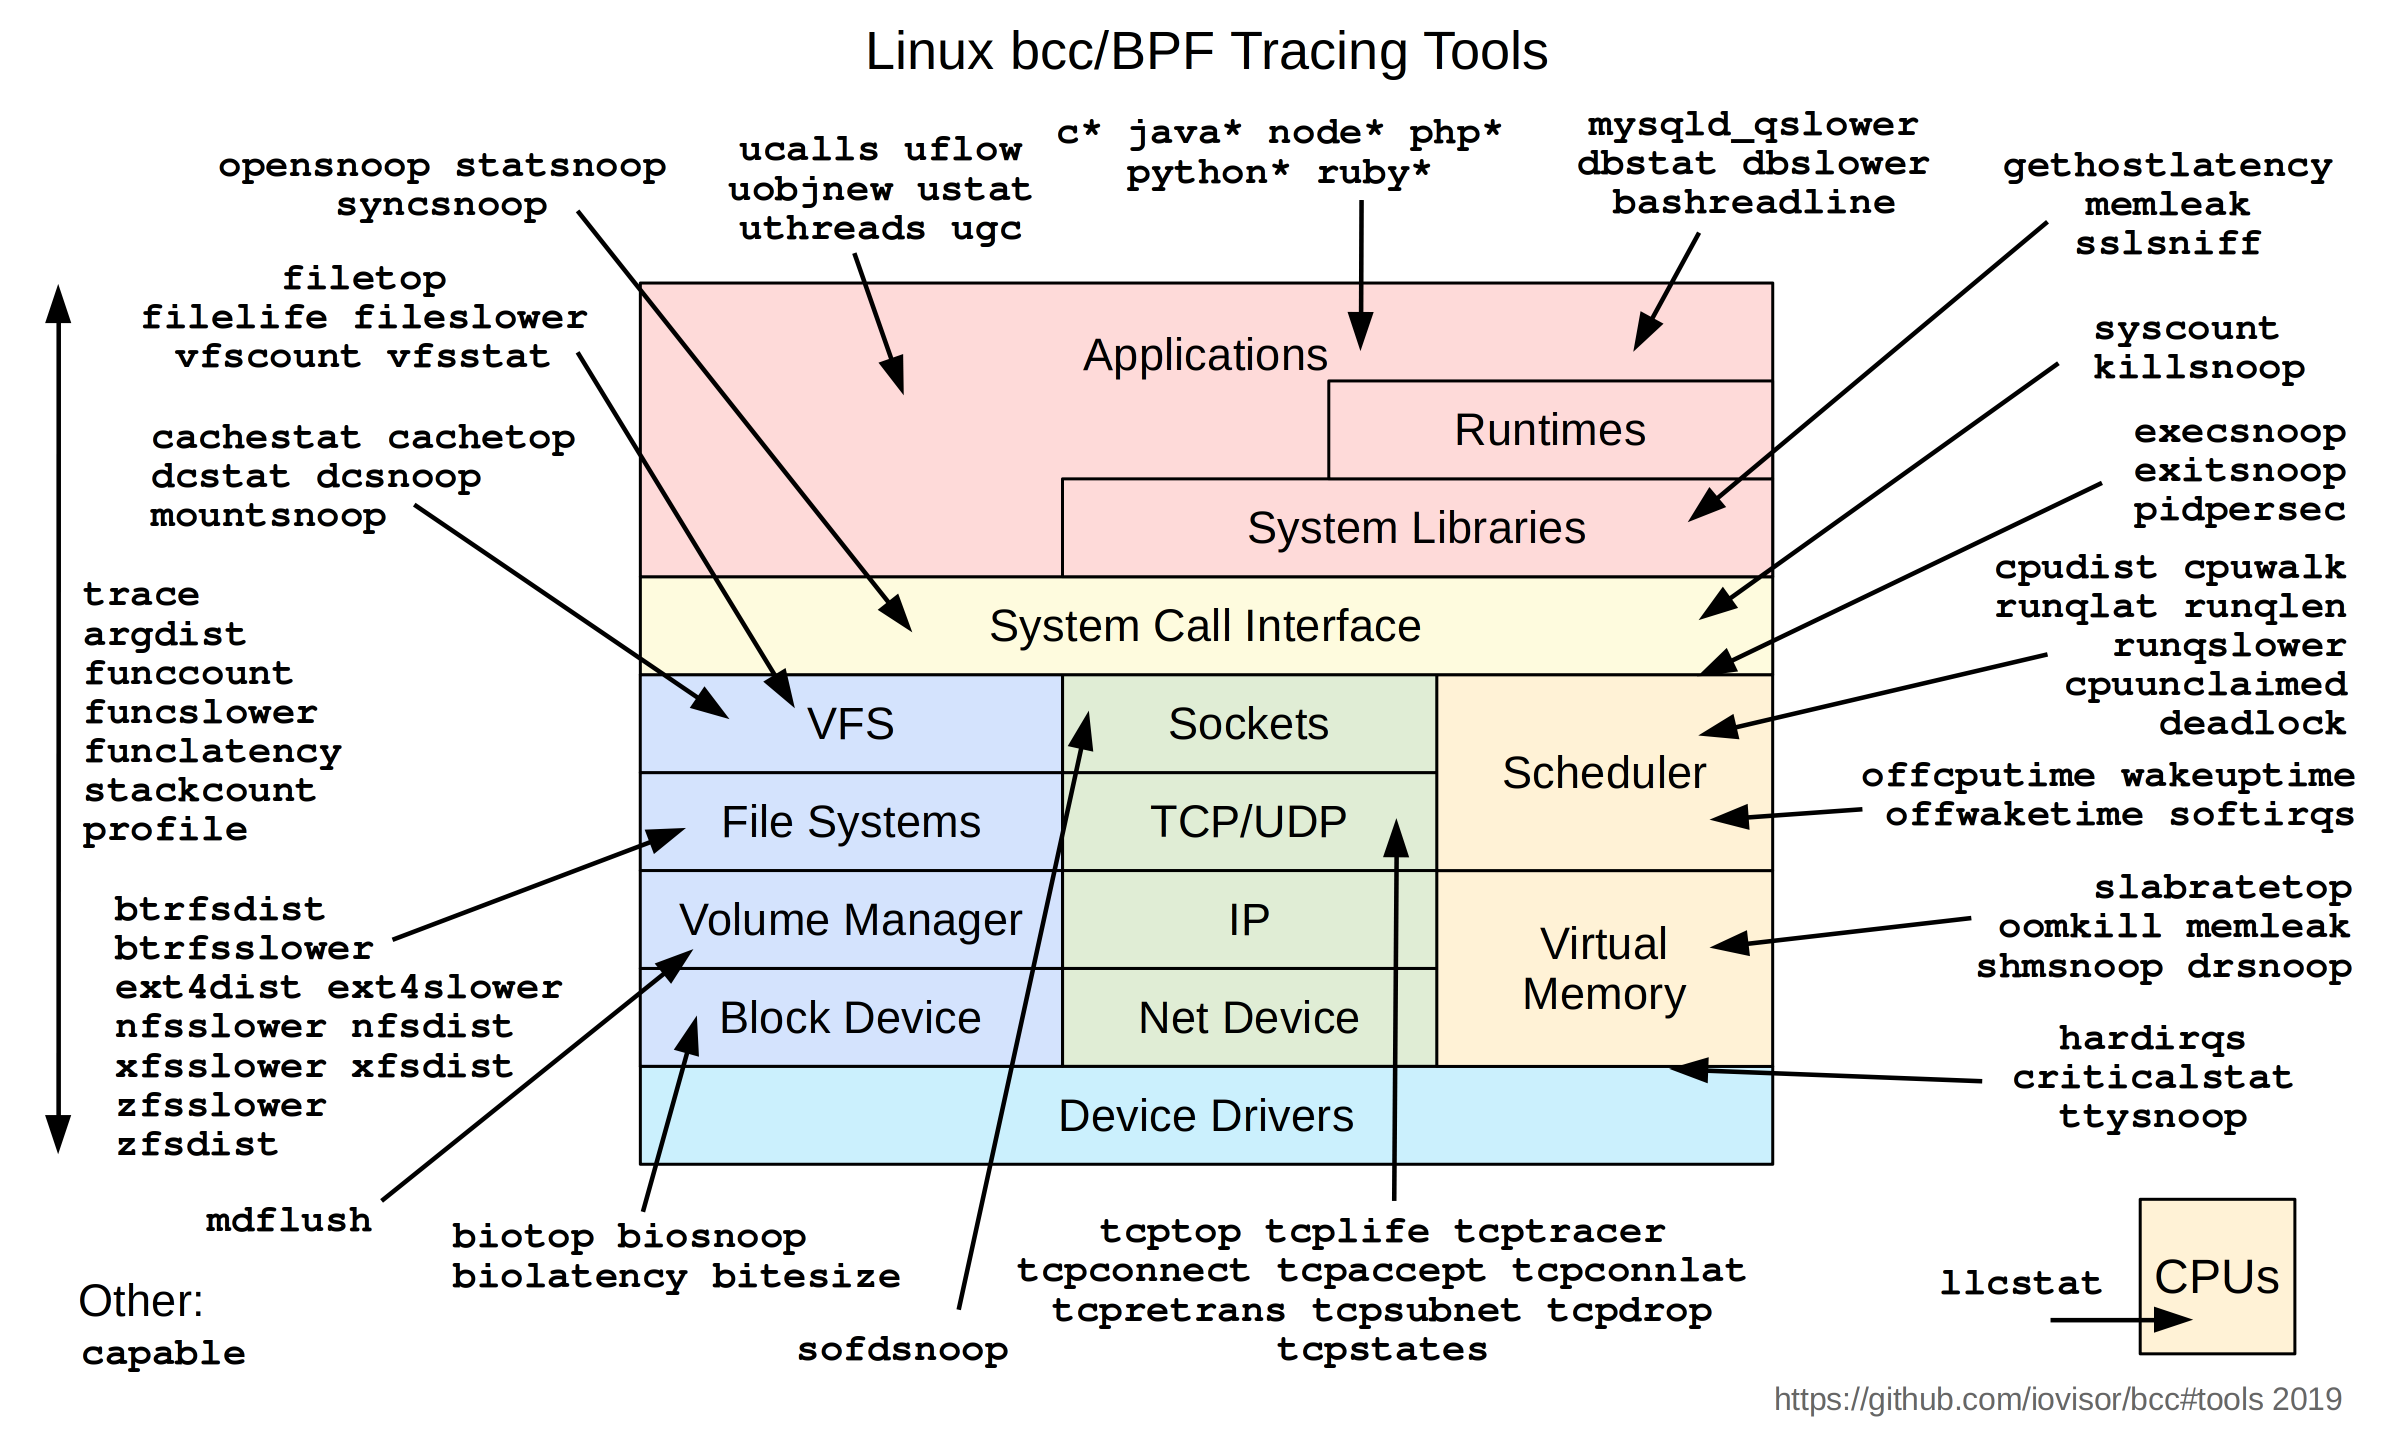
\includegraphics[width=1.0\textwidth]{resources/images/bcc_tracing_tools_2019.png}
%     \caption{A wide range of Linux eBPF-based tracing tools \cite{iovisor_page}.}\label{fig:sota:tracing_tools_linux}
% \end{figure}

\subsection{AF\_XDP socket}
\ac{xdppage} is a type of Linux socket that utilizes \ac{ebpf} to deliver incoming raw network packets arrived from a \ac{NIC} to user space with comparable performance to \ac{dpdkpage} \cite{karlsson_path_to_dpdk_speednodate}. 
The socket has demonstrated the capability to fully utilize a 100Gb line per core on modern CPUs, with impressive baseline packet drop rates of up to 24 million packets per second (Mpps) compared to 4.8Mpps with Linux network stack \cite{hoiland_jorgensen_express_2018} \cite{intel_dpdk_perf}.
This high throughput potential allows us to establish multi-hundreds Gb connections (tunnels) by leveraging a few readily available 40/100Gb NICs, presenting a valuable opportunity for enhanced network performance.

\begin{figure}[H]
	\centering
	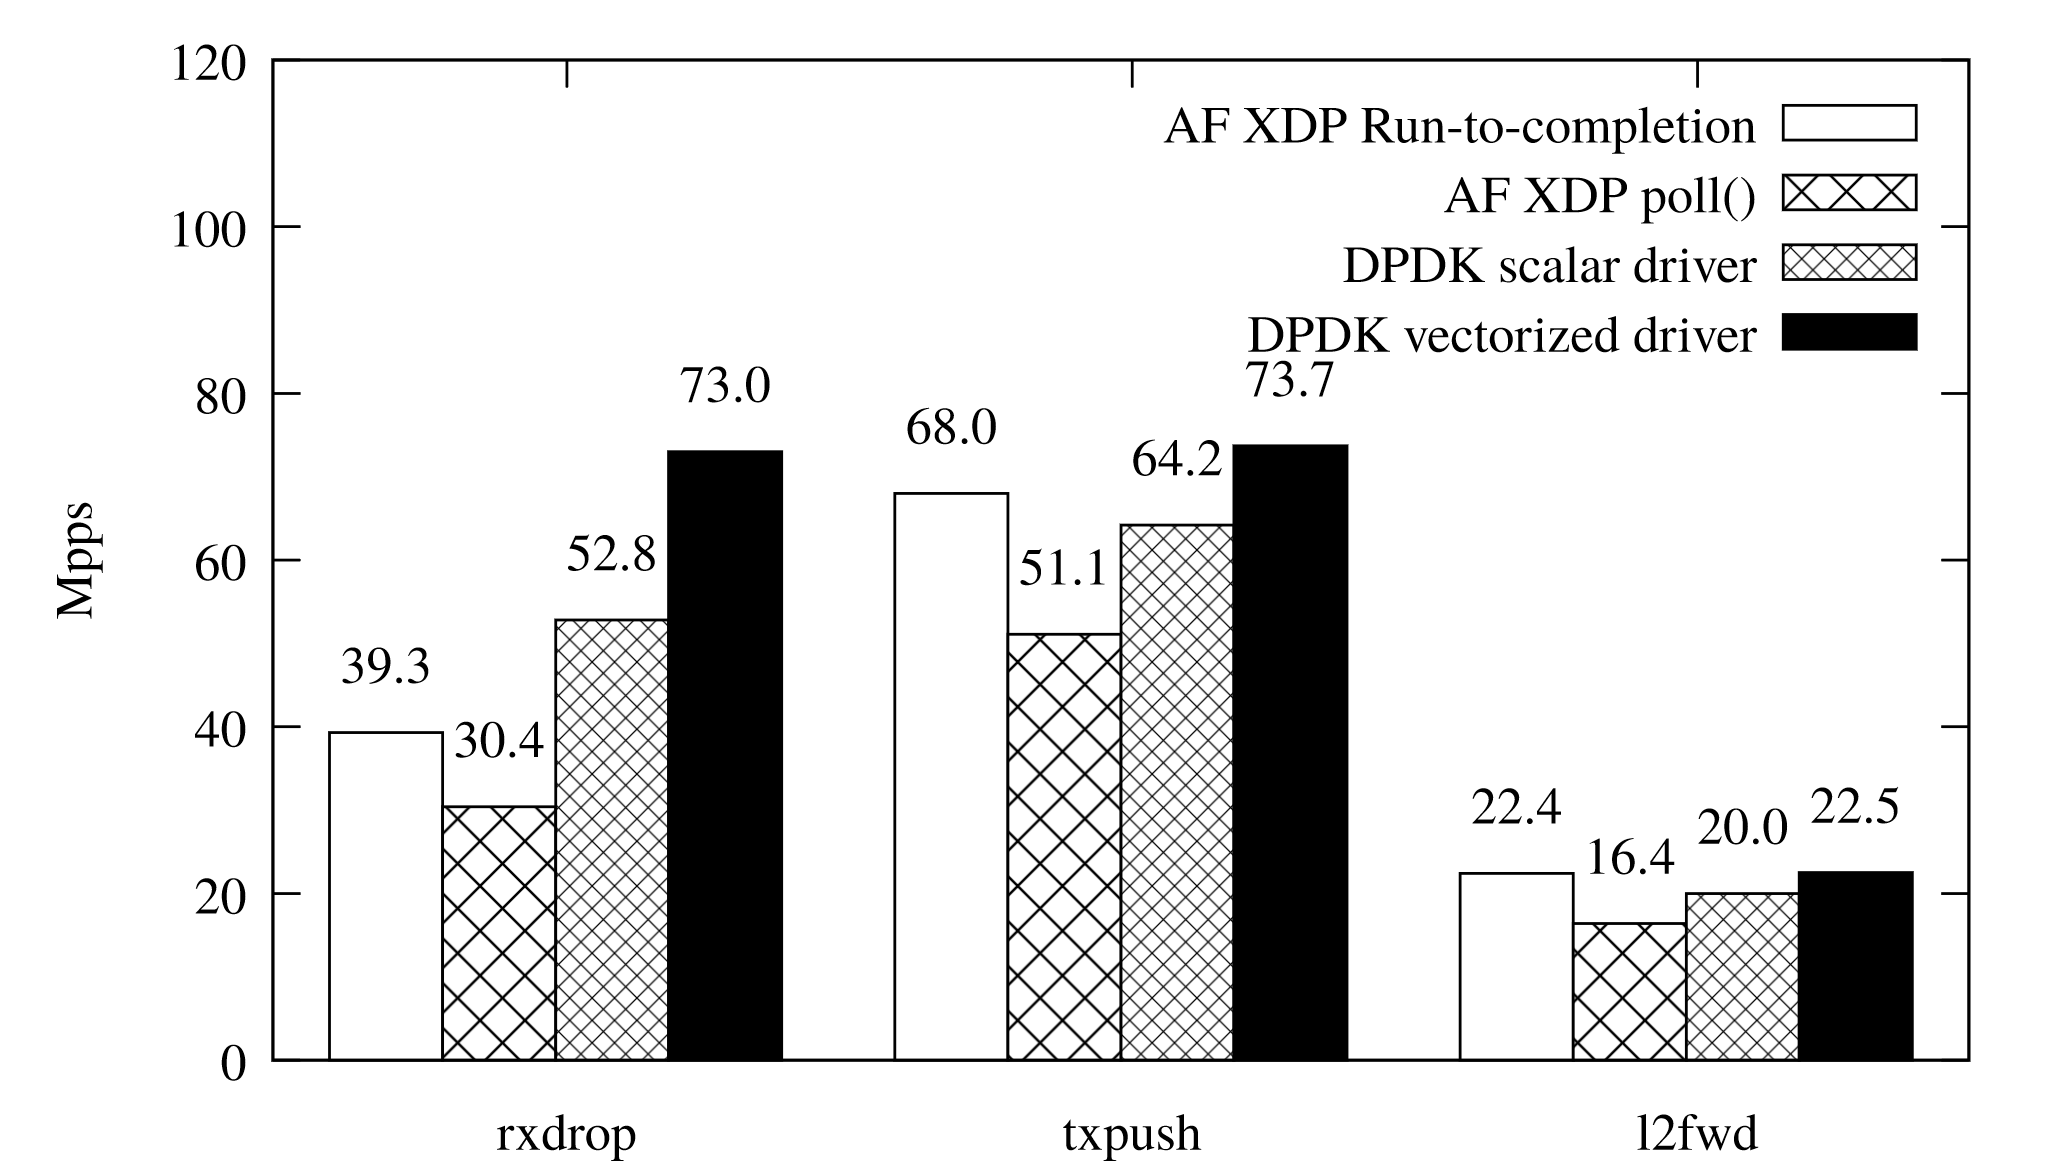
\includegraphics[width=0.8\textwidth]{af_xdp_vs_dpdk_3_micro_benchmarks.PNG}
	\caption{Comparing performance between \ac{xdppage} and \ac{dpdkpage} \cite{karlsson_path_to_dpdk_speednodate}. The authors tested  rxdrop (dropping all arriving packets), txpush (pushing packets out a NIC) and l2fwd (Level-2-forwarding, replacing MAC address of incoming packets and pushing them out) scenarios. DPDK continues to be the leading solution in terms of raw performance.}\label{fig:sota:af_xdp_vs_dpdk_3_micro_benchmarks}
\end{figure}

Being a native Linux's feature, \ac{xdppage} has several advantages over other 3rd party solutions:
\begin{itemize}
	\item Reducing dependency: minimizing the reliance on third-party libraries reduces the concern for potential vulnerabilities.Furthermore, this approach guarantees the longevity of the product, as the socket is maintained by the dedicated team of kernel developers, indicating that the project is unlikely to be discontinued in the near future. 
	\item License: no special license required. However, the eBPF kernel program must be licensed under GNU \ac{GPL} since anything uses eBPF in kernel space is considered a derivative work \cite{gpl_email_discussion} \cite{linux_license_rule} \cite{lwn_clarify_bpf_license}.
	\item Security and Update: the open-source and collaborative nature of Linux ensures that its code base is diligently maintained by dedicated maintainers and an active community of contributors, including researcher from universities and institutes, employee from industrial vendors and individual hobbyist.
\end{itemize}

% \begin{figure}[H]
% 	\centering
% 	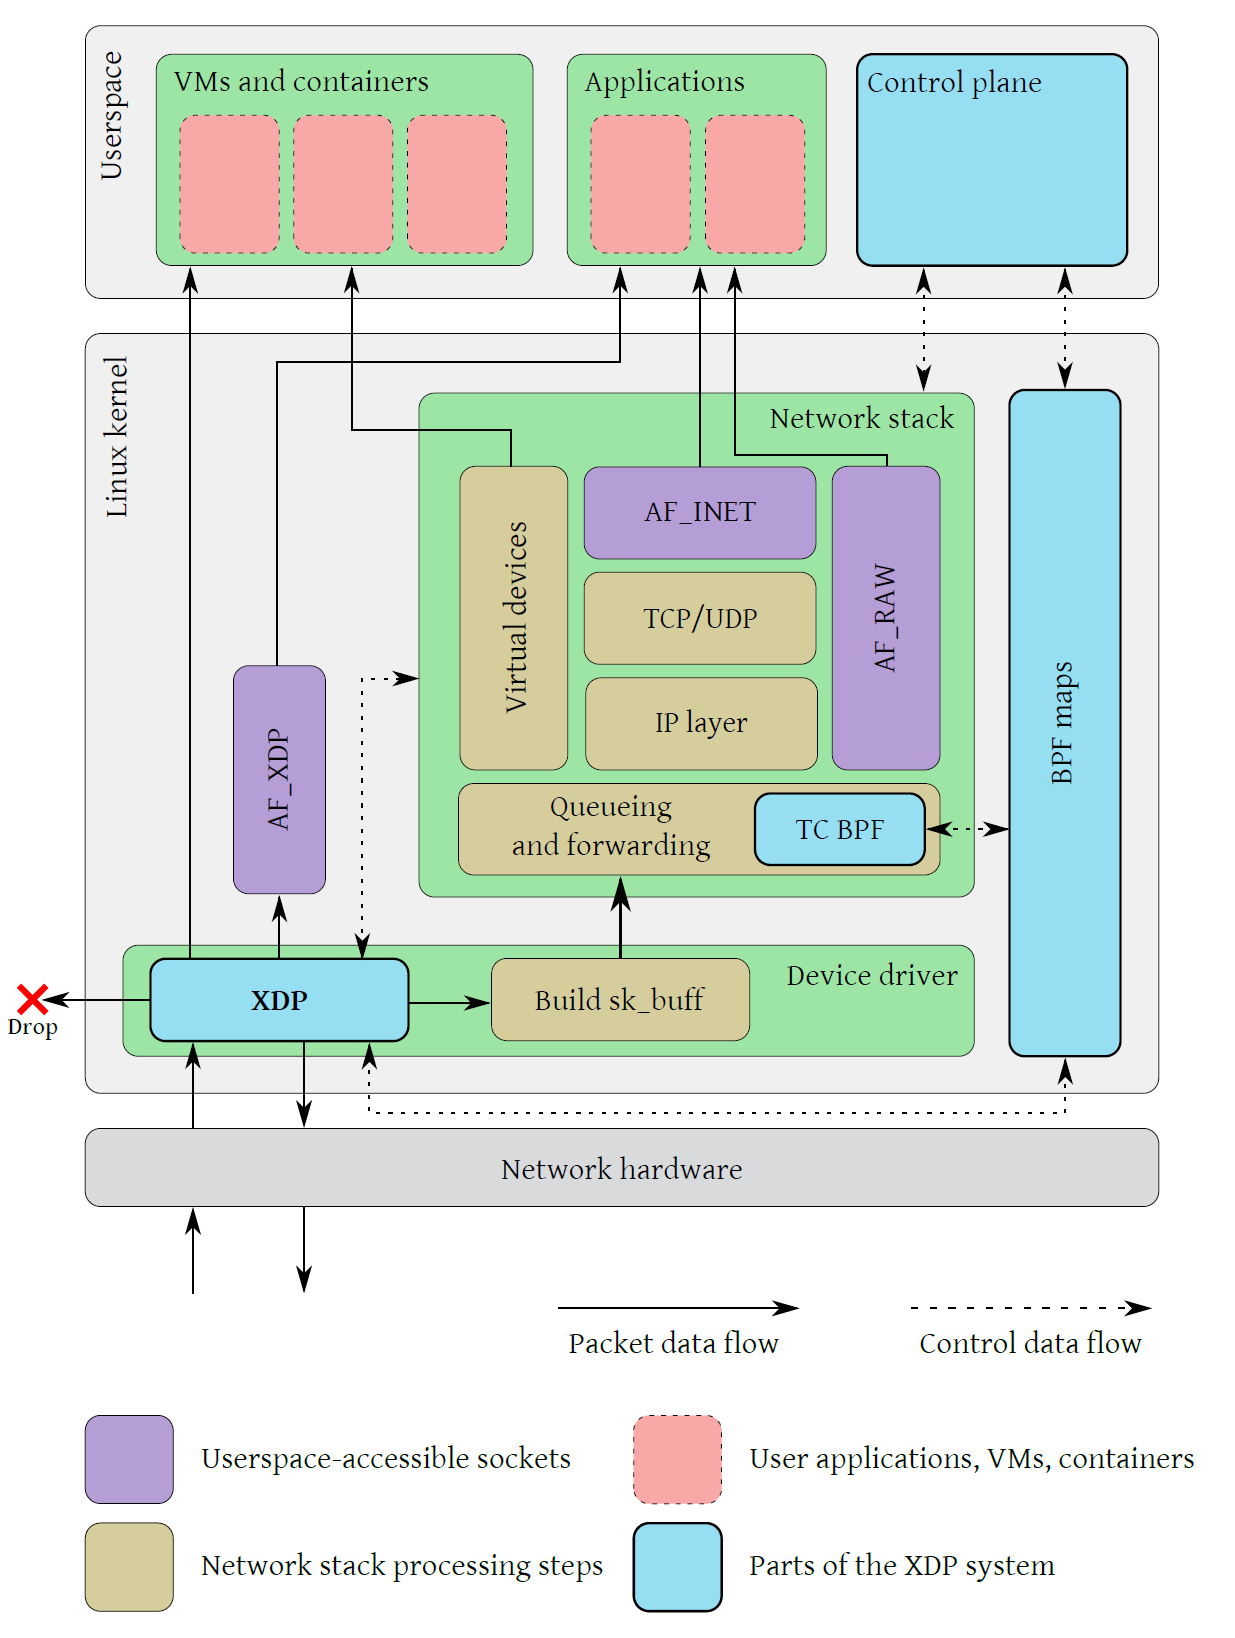
\includegraphics[width=1.0\textwidth]{XDP_integration_with_the_Linux_network_stack.PNG}
% 	\caption{XDP’s integration with the Linux network stack \cite{hoiland_jorgensen_express_2018}. The XDP program is activated whenever a packet enter the driver's buffer, where it will be examined. The XDP program makes the decision if the packet should follow its normal path in the network stack, or be discarded/forwarded/delivered to XDP user space program.}\label{fig:sota:xdp_architecture}
% \end{figure}


    \cleardoublepage\chapter{Related Work}\label{sec:related_work}\minitoc\vspace{.5cm}\index{SotA}

\section{Introduction}

% \begin{wrapfigure}{r}{0.2\textwidth}
%     \centering
%     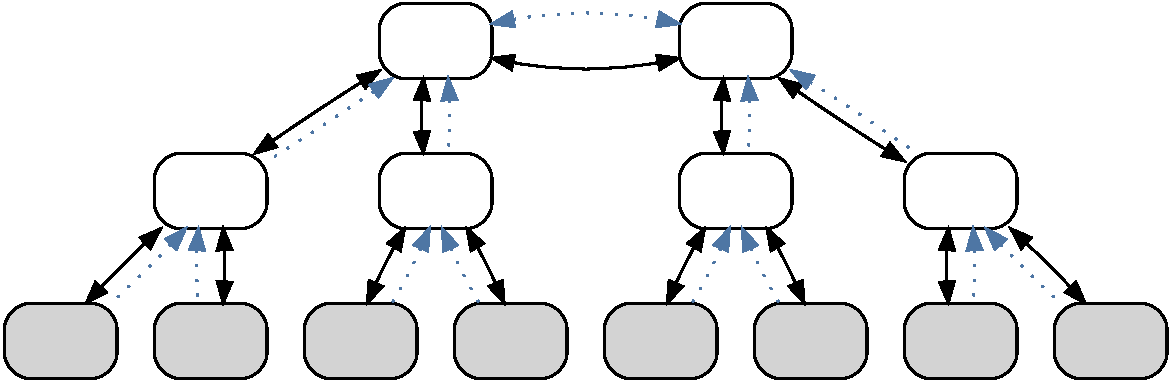
\includegraphics[width=0.2\textwidth]{resources/images/example3}
% \end{wrapfigure}

% \sidenote{Overview}
% \todomid{write}

The concept of multipath is well-established, and in this section, we will explore notable existing multipath protocols, their characteristics, and highlight the unique aspects of our concept. 
Additionally, we will discuss future use cases for our \ac{MTX} and examine current solutions and technologies being utilized. 
Finally, we will take a closer look at the design of the 5G system, with a specific focus on the Data Plane, to explain our plan for showcasing the multipath tunnel using the \ac{gptu} protocol.

\section{Tunneling}\index{Tunneling}
\todo{these following are my words, but do I need cite here?}
The concept of a tunnel draws inspiration from its real-world counterpart, which refers to a confined pathway constructed to direct transportation between two points, separate from the surrounding terrain. 
In the physical sense, tunnels are often excavated deep beneath the earth's surface to bypass obstacles like mountains, rivers, or ocean channels.
In the realm of networking, a tunnel can be perceived as a direct network pathway that enables access to another network from the network to which it is currently connected. 
From an infrastructure standpoint, a tunnel serves as an abstraction layer that abstracts the actual traffic routing from the application and isolates the tunnel's traffic from public network traffic. 
This is typically achieved by encapsulating the application's data packets within the tunnel's packets, and then extracting the original data at the other end of the tunnel.
Many tunnel protocols exist for different purposes: IPv4/IPv6 tunnels to enable compatibility between exclusive networks \cite{rfc4380_Teredo_ipv6_tunnel_udp}, Secure Shell (SSH) - tunnel for remote access and data transfer \cite{rfc4251_ssh_protocol}, and \ac{VPN} tunneling - used for access other network from another network. 
\ac{VPN}s are frequently utilized to remotely access a private network, such as connecting to university's network from home. 
It also functions to conceal the origin of network traffic by making it appear as if it originates from the VPN server, which is useful for bypassing firewalls or restrictions applied by local network providers.
The traffic can also be encrypted to add an extra layer of protection while accessing networks over untrusted connections, like public WLAN provided by coffee shops.
There are several widely recognized VPN protocols, including WireGuard, OpenVPN, IPsec, Cisco AnyConnect VPN, L2TP/IPsec, SSTP (Secure Socket Tunneling Protocol), ... each embodies its unique philosophy, background, and intended field of application.


\section{Multipath Connection}\index{Multipath Connection}\label{sec:related_work:mp_connection}
Our primary emphasis is on establishing a connection between two points, irrespective of the number of physical transportation links.
% We will explore various protocols that implement the concept and make comparisons with our approach.
There are 2 approaches to utilize multiple links: managing multiple underlying connections created by existing protocols (\ac{MPTCP} with TCP), and creating a new multipath protocol \ac{SCTP}.
Drawing inspiration from these protocols, our design of \ac{MTX} adopts a hybrid approach: a tunnel that transfers data over multiple UDP connections instead of maintaining TCP sessions. 
The tunnel comprises two primary logical components: the control plane and the transport plane. 
The control plane handles session management, congestion control overhead, and other administrative tasks, enabling the transport plane to be constructed with wrappers over UDP sockets.
Unlike serving solely the socket caller, the multipath tunnel is designed to offer connection and flow management for multiple applications, enabling centralized resource management and scheduling.

\subsection{Multipath TCP}\label{sec:related_work:mp_connection:MPTCP}
% MultiPath TCP (MPTCP) is an effort towards enabling the simultaneous use of several IP-addresses/interfaces by a modification of TCP that presents a regular TCP interface to applications, while in fact spreading data across several subflows. Benefits of this include better resource utilization, better throughput and smoother reaction to failures. 

\ac{MPTCP} is is a major extension to TCP to decoupling TCP from the transport layer by utilizing multiple sub flows, which are underlying TCP connections \cite{Bonaventure_mptcp_decoupling}.
The protocol is showcased in both mobile and data center environments, serving distinct objectives. 
In addition to enhancing data center performance by employing \ac{MPTCP}'s distributed load-balancing across multiple paths, the protocol also provides redundancy and effective congestion management capabilities \cite{raiciu_improving_nodate}.
In the context of mobile hand-over capability, \ac{MPTCP} enhances the ability to maintain TCP sessions while the user equipment moves continuously. 
For instance, a smartphone can continue utilizing both LTE and Wi-Fi connections for a TCP session and predict the optimal route for transmitting most of the traffic. 
By monitoring the radio signal strength, it becomes possible to anticipate potential disruptions in the Wi-Fi connection or when a user enters a building and encounters a loss of cellular signal. 
The author argues that although maintaining two radios simultaneously consumes more power, it can potentially reduce the time required to establish new connections and transmit data \cite{paasch_multipath_2014}.

\begin{figure}[H]
	\centering
	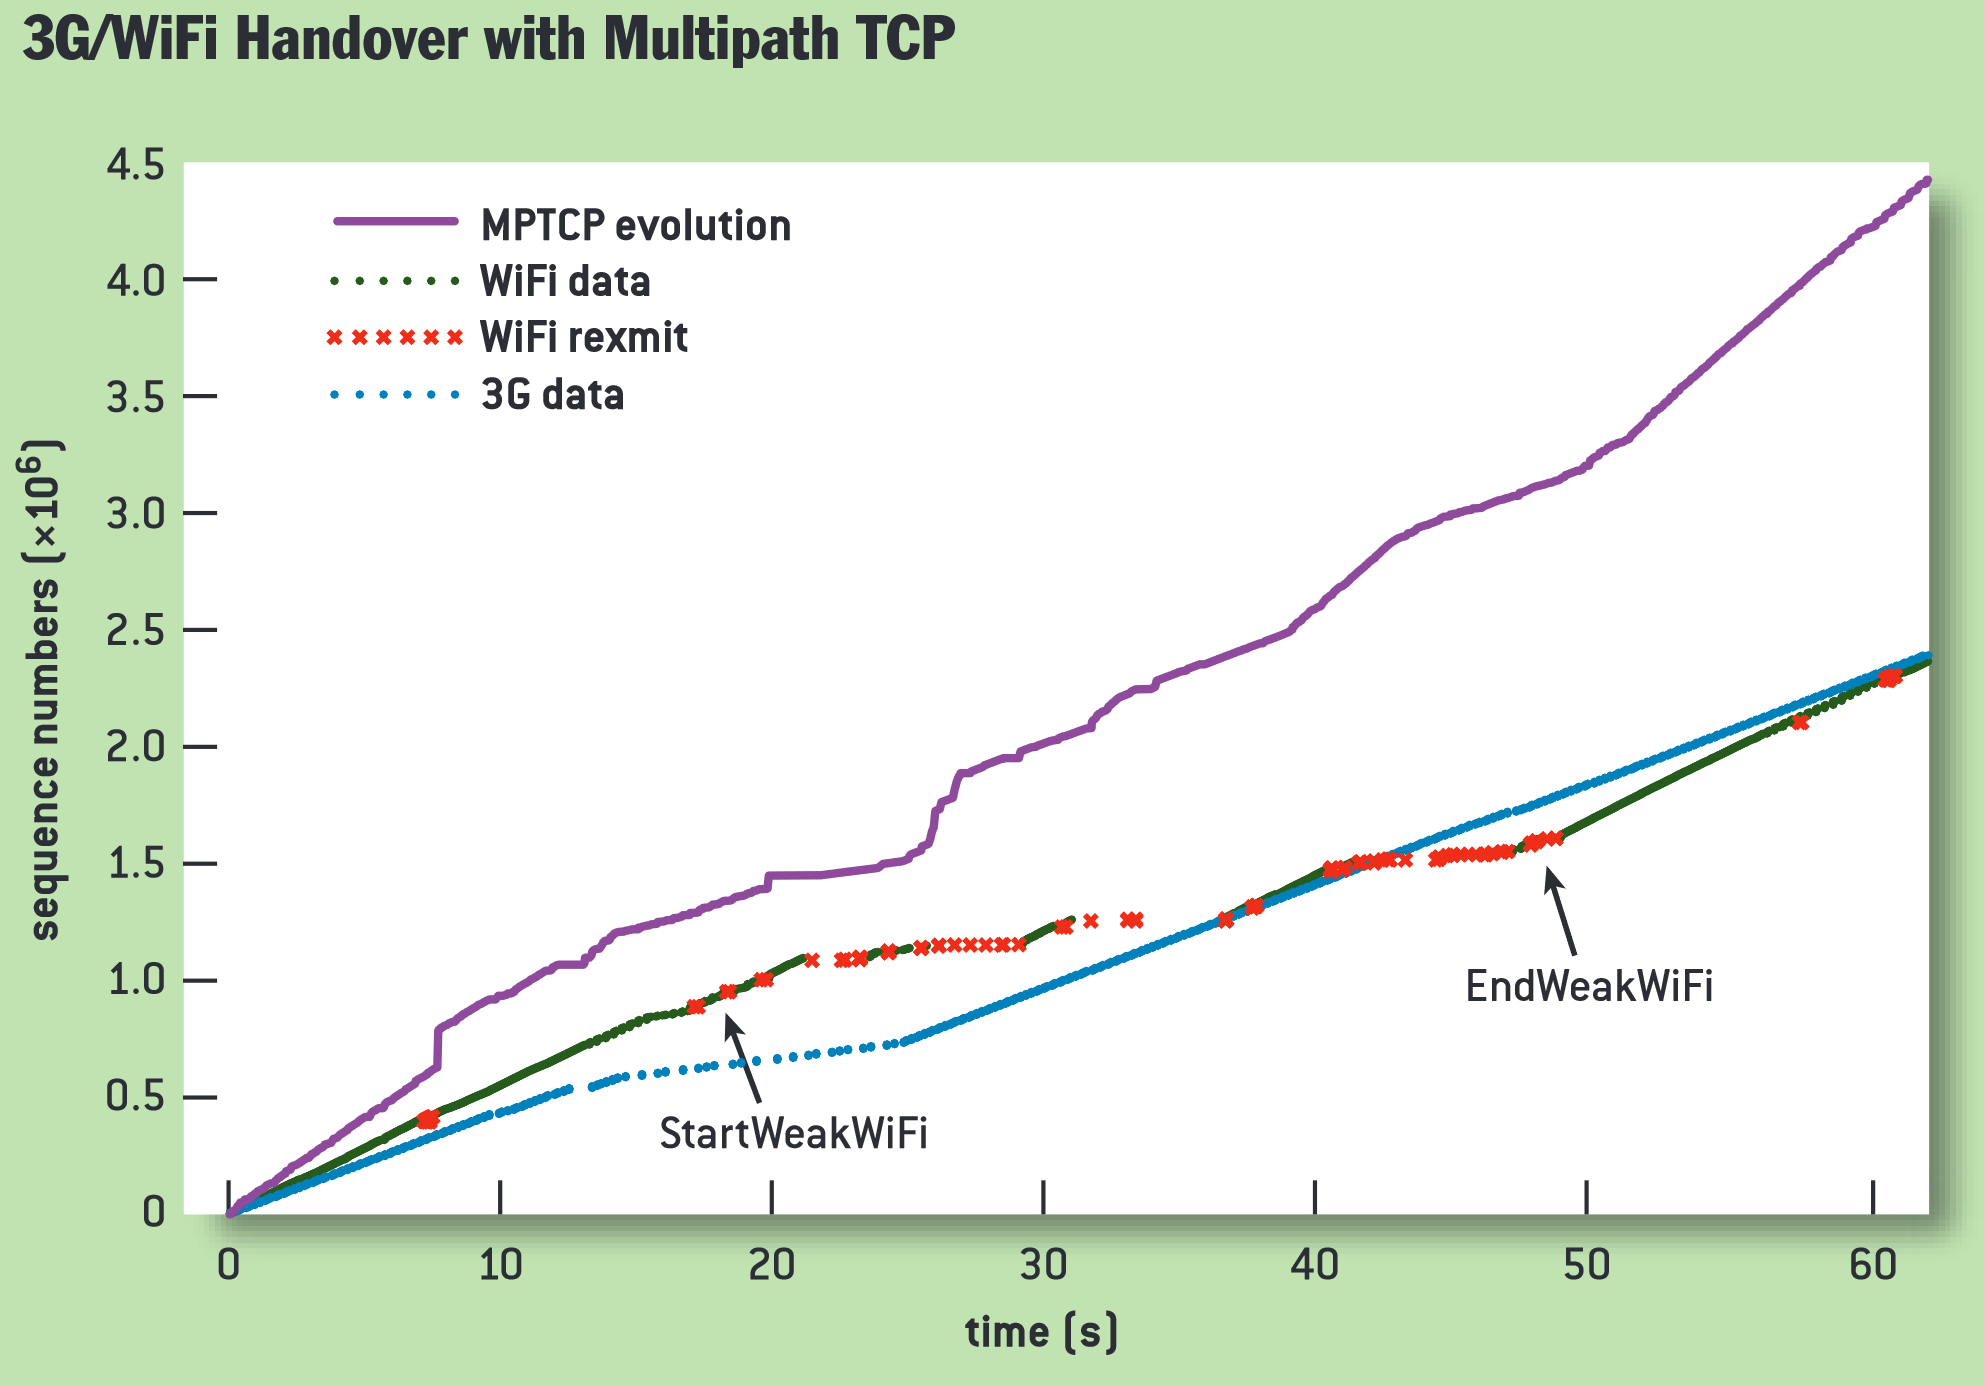
\includegraphics[width=1.0\textwidth]{resources/images/3G_WiFi_Handover_with_Multipath_TCP.PNG}
	\caption{3G/WiFi Handover with Multipath TCP \cite{paasch_multipath_2014}. The MPTCP connection persists despite of WiFi and 3G's unreliable connections. A weak WiFi signal can be indicative of the device moving beyond the coverage range of the router. The command \textit{REXMIT} changes the time-out value for each packet which is used for retransmitting packet.}
    \label{fig:related_work:3G_WiFi_Handover_with_Multipath_TCP}
\end{figure}

\subsection{Stream Control Transmission Protocol}\label{sec:related_work:mp_connection:SCTP}
\ac{SCTP} introduces multiple addresses to the transport layer, which serves as failover and simultaneous underlying connection.
Unlike \ac{MPTCP}, existing internet's infrastructure such as firewalls, routers were not designed to handle \ac{SCTP}'s packets and thus severely limits usage of the protocol \cite{paasch_multipath_2014}. 
Notably, \ac{SCTP} is used in 5G core design for transmitting messages in Control plane.

\begin{figure}[H]
	\centering
	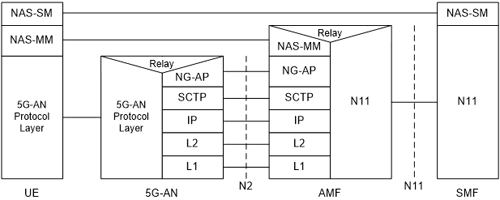
\includegraphics[width=0.8\textwidth]{resources/images/3gpp_5g_part_of_control_plane_protocol.png}
	\caption{Control Plane protocol stack between the UE, the 5G-AN, the AMF and the SMF \cite{3gpp_5g_system_overview}}
    \label{fig:related_work:3gpp_5g_part_of_control_plane_protocol}
\end{figure}


\section{5G Deployment}\index{5G Deployment}
5G services and functions are designed to be deployed in containers and virtual machines, often on server-grade general purpose computers.

These components are categorized into two groups: the Control plane and the Data plane.

As mentioned in \Cref{sec:related_work:mp_connection:SCTP}, \ac{SCTP} protocol with multipath support is used in control plane.
The Data plane relies on \ac{gptu} protocol with \ac{UDP} as the transport protocol to exchange high volume of data between \ac{UPF} and \ac{DN}

\begin{figure}[H]
	\centering
	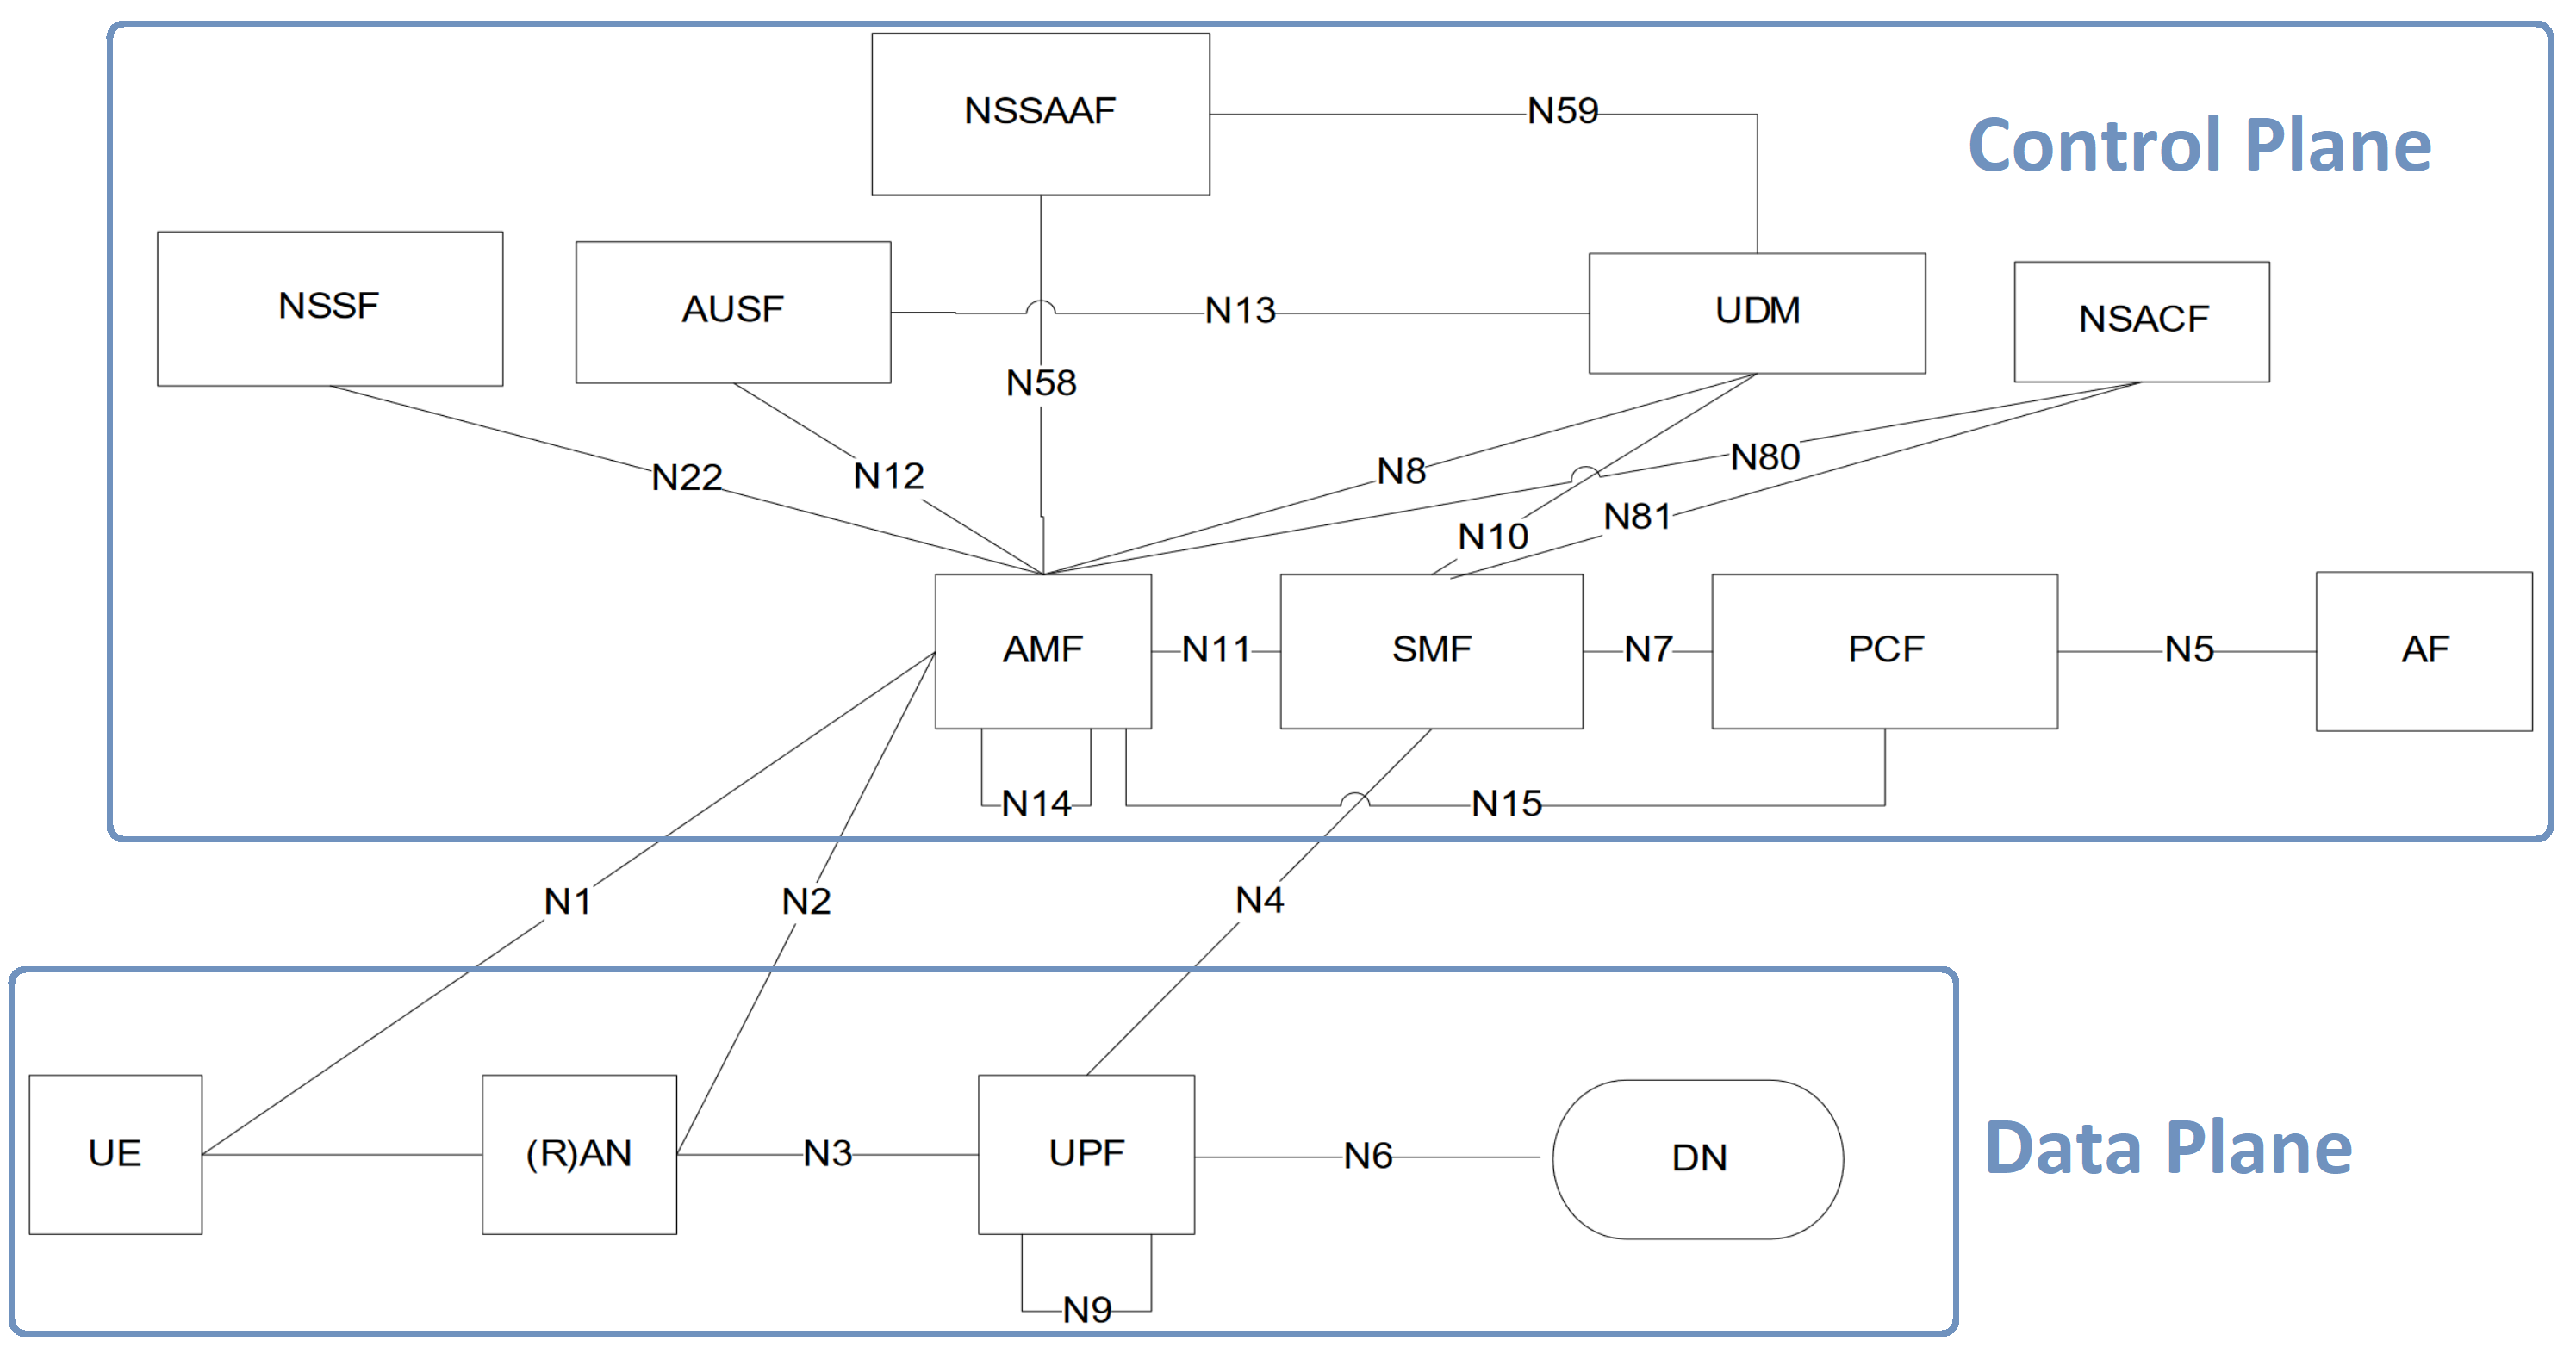
\includegraphics[width=1.0\textwidth]{resources/images/Non_Roaming_5G_System_Architecture_in_reference_point_representation.png}
	\caption{Non-Roaming 5G System Architecture in reference point representation \cite{3gpp_5g_system_architect_spec_release_18}}
    \label{fig:related_work:Non_Roaming_5G_System_Architecture_in_reference_point_representation}
\end{figure}



% \begin{figure}[H]
%     \centering
%     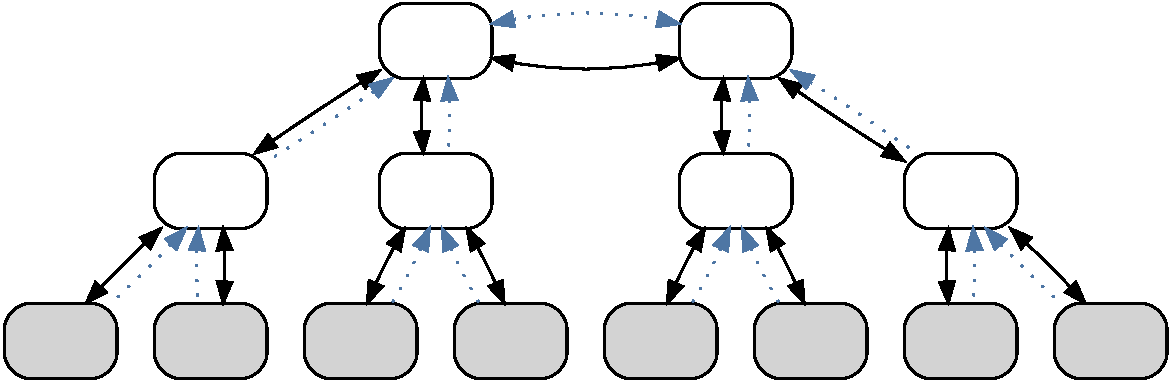
\includegraphics[width=.55\textwidth]{resources/images/example3}
%     \caption{Related area 1 within the structure of research}\label{fig:hourglass:ra1}
% \end{figure}

% \sidenote{Overview}
% \todomid{write about \Cref{fig:hourglass:ra1}}

% \sidenote{Focus}
% \todomid{write}

% \subsection{Specific Example 1}

% \sidenote{Definition}
% \todomid{write}

% \sidenote{Issues}
% \todomid{write}

% \subsection{Specific Example 2}

% \sidenote{Definition}
% \todomid{write}

% \sidenote{Implementations}
% \todomid{write}

% \sidenote{Research}
% \todomid{write}

% \sidenote{Standards}
% \todomid{write}

% \sidenote{Adoption}
% \todomid{write}

% \subsection{Specific Example 3}\index{Example 3}

% \sidenote{Transition}
% \todomid{write about \Cref{fig:sota:trans}}

% \begin{figure}
%     \centering
%     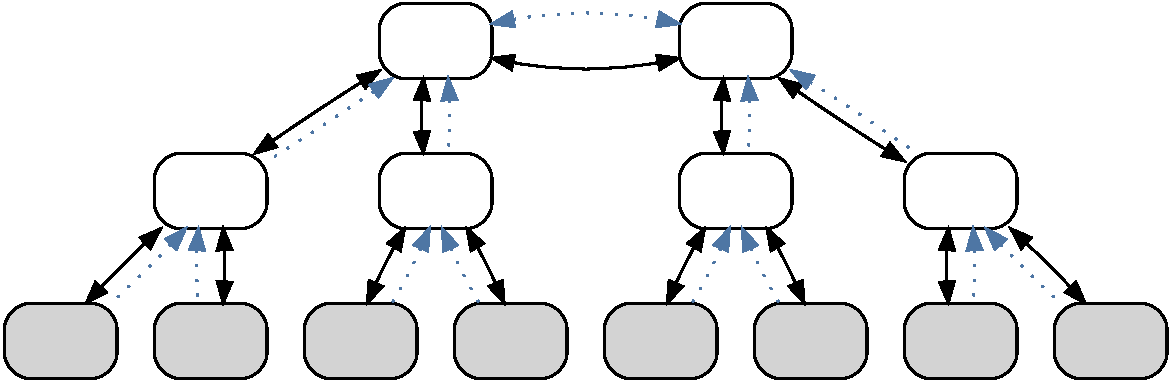
\includegraphics[width=.85\textwidth]{resources/images/example3}
%     \caption{Comparison of Example 2 and Example 3 (based on~\cite{li2002design})}\label{fig:sota:trans}
% \end{figure}

% \sidenote{Standards}
% \todomid{write}

% \sidenote{Extension}
% \todomid{write}

% \sidenote{Other Standards}
% \todomid{write}

% \sidenote{Something}
% \todomid{write}

% \sidenote{Something}
% \todomid{write}

% \sidenote{Something}
% \todomid{write}

% \sidenote{Something}
% \todomid{write}

% \sidenote{Something}
% \todomid{write}

% \sidenote{Something}
% \todomid{write}

% \section{Related Area 2}\index{Related Area 2}

% \sidenote{Overview}
% \todomid{write}

% \sidenote{Focus}
% \todomid{write about \Cref{fig:sota:ra2}}

% \begin{figure}[!hbtp]
%     \centering
%     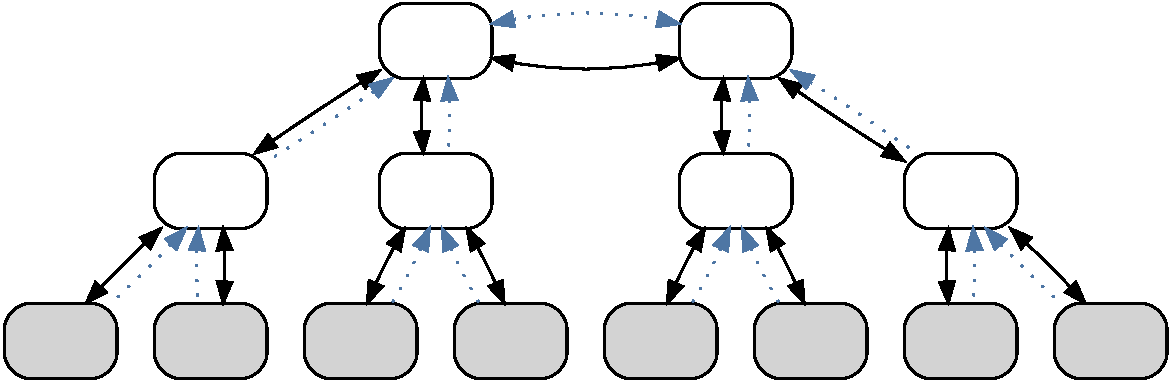
\includegraphics[width=1\textwidth]{resources/images/example3}
%     \caption{Related Area 2}\label{fig:sota:ra2}
% \end{figure}

% \sidenote{Something}
% \todomid{write}

% \subsection{Specific Example 1}

% \sidenote{Definition}
% \todomid{write}

% \sidenote{Issues}
% \todomid{write}

% \subsection{Specific Example 2}

% \sidenote{Definition}
% \todomid{write}

% \sidenote{Implementations}
% \todomid{write}

% \sidenote{Research}
% \todomid{write}

% \sidenote{Standards}
% \todomid{write}

% \sidenote{Adoption}
% \todomid{write}


% \section{Related Area 3}\index{Related Area 3}

% \sidenote{Overview}
% \todomid{write}

% \sidenote{Focus}
% \todomid{write about \Cref{fig:sota:ra3}}

% \begin{figure}[!hbtp]
%     \centering
%     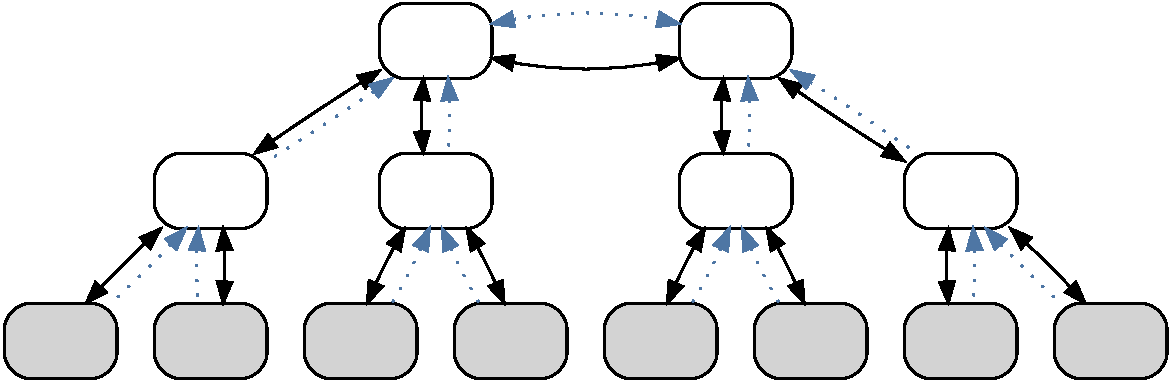
\includegraphics[width=1\textwidth]{resources/images/example3}
%     \caption{Related Area 3}\label{fig:sota:ra3}
% \end{figure}

% \sidenote{Something}
% \todomid{write}

% \subsection{Specific Example 1}

% \sidenote{Definition}
% \todomid{write}

% \sidenote{Issues}
% \todomid{write}

% \subsection{Specific Example 2}

% \sidenote{Definition}
% \todomid{write}

% \sidenote{Implementations}
% \todomid{write}

% \sidenote{Research}
% \todomid{write}

% \sidenote{Standards}
% \todomid{write}

% \sidenote{Adoption}
% \todomid{write}

% \section{Conclusion}

% \sidenote{Summary}
% \todomid{write}

% \sidenote{Takeaway 1}
% \todomid{write}

% \sidenote{Takeaway 2}
% \todomid{write}

% \sidenote{Takeaway 3}
% \todomid{write}

% \sidenote{Next chapter}
% \todomid{write}

    % \cleardoublepage
\chapter{Requirement Analysis}\label{sec:reqs}\minitoc\vspace{.5cm}
\index{Requirements}

% https://www.cs.fsu.edu/~lacher/courses/COP3331/rad.html
\section{Introduction}
The objective of this project is to conduct research and implement the concept of a multipath networking tunnel utilizing the \ac{xdppage} technology. The project aims to deliver a comprehensive thesis documentation along with a functional implementation, preferably in the form of a test program based on the \ac{MTX} tunnel designed as a programming library.
This \ac{MTX} library will enable the establishment of a network tunnel between two machines, allowing traffic to flow simultaneously over multiple network links. 
The test program will serve as a demonstration platform for the library, simulating a transport session using the \ac{gptu} protocol — a 5G technology employed for tunneling a significant volume of non-homogeneous data.
During the demonstration, the library's capabilities will be showcased, including flow management, throughput control, and other essential features that align with the intended purpose of the library.

\section{Current solution}
% Multipath is equivalent to horizontal scaling to increase connection capacity.
% It is also a method to achieve better reliability by building redundancy.
% Quality of service can also be improve by providing treatment and links optimized for different data flows.
% By establishing a multipath tunnel, the resources of each path can be monitored and scheduled between concurrent applications and leads to better utilization and efficiency.
Multipath technique serves as a means of horizontally scaling networking capacity by aggregating resources to increase connection bandwidth. 
Additionally, it offers a way to enhance reliability by incorporating redundancy into the network connection. Furthermore, multipath can improve quality of service by enabling optimized treatment and dedicated links for different types of data flows.
Finally, through the establishment of a multipath tunnel, the resources available on each path can be monitored and efficiently allocated among concurrent applications. 
This leads to improved resource utilization and overall efficiency in the network.

Current tunnel and VPN solutions available in the market are limited to single-path functionality. While protocols like \ac{MPTCP} and \ac{SCTP} are well-known for their multipath capabilities, they are primarily designed for exclusive use by a single caller.
Our focus lies in exploring how high-demand applications, particularly within the 5G infrastructure, handle the substantial traffic volume. Interestingly, certain implementations leverage DPDK to enhance packet forwarding and processing capabilities beyond the limitations of the Linux network stack. However, these software stacks are not readily accessible for research and testing purposes without purchasing expensive system.

\section{Proposed solution}
To address the need for a multipath connection that supports non-homogeneous and concurrent usage, we introduce the concept of a multipath tunnel. 
Our proposal aims to bridge the gap by enabling the utilization of multiple paths simultaneously.
To ensure optimal path utilization and minimal latency, we will utilize \ac{xdppage} technology to handle the movement of tunnel traffic. 
Specifically, the tunnel traffic will consist of UDP packets, allowing for efficient and effective data transmission.
The following section will present the requirements for the project \todo{improve}.

\subsection{Functional requirements}
% Functional requirements describes the high-level functionality of the system.
We define the functional requirements for the \ac{MTX} library:
\begin{itemize}
    \item Given multiple \ac{NIC}s, \ac{MTX} library shall be able to establish a tunnel between 2 hosts and exchange data through the tunnel over the chosen \ac{NIC}s.
    \item The \ac{MTX} library shall send and receive tunnel's UDP packets using \ac{xdppage} socket exclusively.
    \item The\ac{MTX} library shall support for path-level control and treatment, including scheduling, path failure detection and initiation. \todo{more}
    \item The\ac{MTX} library shall provide support for flow-level control and treatment, including setting and enforcing priority, traffic shaping, resource allocation for sensitive requirement (i.e path for low latency data).
    \item A centralized controller shall be provided. Users shall have access to configuration options for the aforementioned features.
\end{itemize}

\subsection{Nonfunctional requirements}
We define the non-functional requirements for the \ac{MTX} library:
\begin{itemize}
    \item Usability: \ac{MTX} library should be used similar to a Linux socket. A global configuration will be responsible for managing the overall configuration of the tunnel. On the other hand, each caller will have the ability to configure the traffic characteristics according to their specific requirements.
    \item Performance and Reliability: The tunnel is expected to deliver throughput asymptotic to the line rate while having very low negative effect on overall system load thanks to \ac{xdppage} technology. Measuring is rather complicated since the code quality can't be ensured and high performance hardware will be needed. This problem should be addressed in the course of the project.
\end{itemize}

\subsection{System models}
Intended to be a general purpose multipath tunnel, \ac{MTX} is designed to be the wrapper around transport layer to abstract the multipath details.
Callers interact with the tunnel through shared memory or a TUN/TAP interface. This will be discussed further.
The library can be considered for application where reliability, high performance and ease of maintain requirements converge \todo{more}.
\todo{System models describes the scenarios, use cases, object model, and dynamic models for the system. This section contains the complete functional specification, including mock-ups illustrating the user interface of the system and navigational paths representing the sequence of screens. The subsections Object model and Dynamic model are written during the Analysis activity.}


% \begin{wrapfigure}{r}{0.2\textwidth}
%     \centering
%     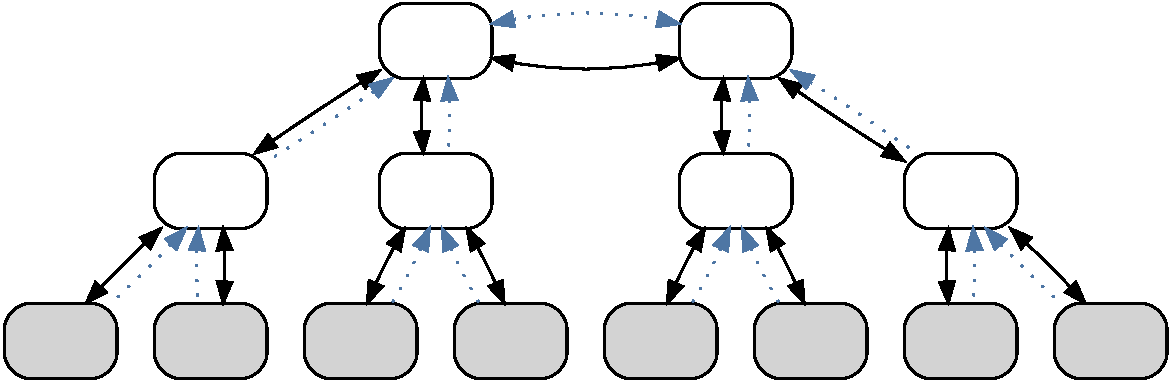
\includegraphics[width=0.2\textwidth]{resources/images/example3}
% \end{wrapfigure}

% \sidenote{Overview}
% \todomid{write about \Cref{fig:req:details}}

% \begin{figure}[H]
%     \centering
%     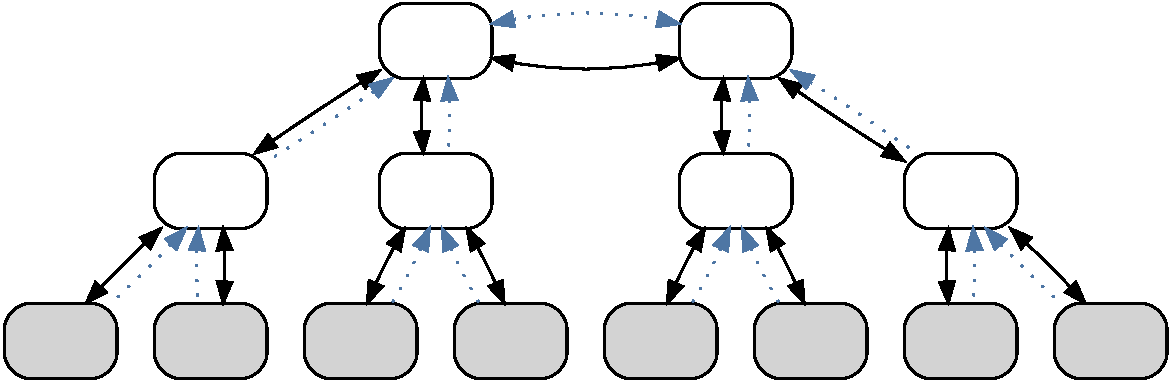
\includegraphics[width=.85\textwidth]{resources/images/example3}
%     \caption{More detailed overview of the requirements}\label{fig:req:details}
% \end{figure}

% \sidenote{Structure of Research}
% \todomid{write about \Cref{fig:hourglass:reqs}}

% \begin{figure}[H]
%     \centering
%     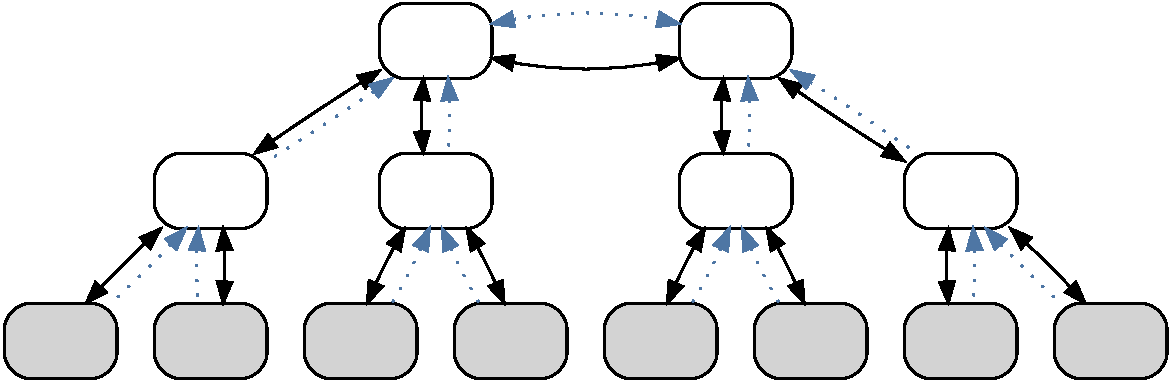
\includegraphics[width=.55\textwidth]{resources/images/example3}
%     \caption{Placement of the requirement section in the structure of research}\label{fig:hourglass:reqs}
% \end{figure}

% \section{Stakeholder 1}

% \sidenote{\Cref{tbl:reqs:stakeholder1}}
% \todomid{write about \Cref{tbl:reqs:stakeholder1}}

% \begin{tabularx}{\textwidth}{lX}
%     \caption{Requirements from stakeholder 1 perspective}\label{tbl:reqs:stakeholder1}\\
%     \toprule
%     \textbf{\#}& \textbf{Description}  \\\midrule
%     \endfirsthead%
%     \toprule
%     \textbf{\#}& \textbf{Description}  \\\midrule
%     \endhead%
%     \requirement{U}{req:stakeholder1:foo}{Foo}
%        & \todomid{write}
%     \\\midrule
%     \requirement{U}{req:stakeholder1:bar}{Bar}
%        & \todomid{write}
%     \\\bottomrule
% \end{tabularx}

% \section{Stakeholder 2}

% \sidenote{\Cref{tbl:reqs:stakeholder2}}
% \todomid{write about \Cref{tbl:reqs:stakeholder2}}

% \begin{tabularx}{\textwidth}{lX}
%     \caption{Requirements from stakeholder 2 perspective}\label{tbl:reqs:stakeholder2}\\
%     \toprule
%     \textbf{\#}& \textbf{Description}  \\\midrule
%     \endfirsthead%
%     \toprule
%     \textbf{\#}& \textbf{Description}  \\\midrule
%     \endhead%
%     \requirement{S}{req:stakeholder2:foo}{Foo}
%        & \todomid{write}
%     \\\midrule
%     \requirement{S}{req:stakeholder2:bar}{Bar}
%        & \todomid{write}
%     \\\bottomrule
% \end{tabularx}

% \section{Stakeholder 3}

% \sidenote{\Cref{tbl:reqs:stakeholder3}}
% \todomid{write about \Cref{tbl:reqs:stakeholder3}}

% \begin{tabularx}{\textwidth}{lX}
%     \caption{Requirements from stakeholder 3 perspective}\label{tbl:reqs:stakeholder3}\\
%     \toprule
%     \textbf{\#}& \textbf{Description}  \\\midrule
%     \endfirsthead%
%     \toprule
%     \textbf{\#}& \textbf{Description}  \\\midrule
%     \endhead%
%     \requirement{T}{req:stakeholder3:foo}{Foo}
%        & \todomid{write}
%     \\\midrule
%     \requirement{T}{req:stakeholder3:bar}{Bar}
%        & \todomid{write}
%     \\\bottomrule
% \end{tabularx}

% \section{Conclusion}

% \sidenote{Summary}
% \todomid{write}

% \sidenote{Takeaway 1}
% \todomid{write}

% \sidenote{Takeaway 2}
% \todomid{write}

% \sidenote{Takeaway 3}
% \todomid{write}

% \sidenote{Next chapter}
% \todomid{write}
    % \cleardoublepage
\chapter{Approach and Design}\label{sec:approach_design}\minitoc\vspace{.5cm}
\index{Approach and Design}

By employing AF_XDP sockets for the Receiver-Transmitter layer (RX-TX), we can achieve multipath tunneling that offers exceptional performance and grants complete control over raw IP packets before they enter the Linux network stack. 
Thanks to the secure design of the eBPF virtual machine architecture, this approach remains safer compared to utilizing kernel modules or kernel code used by Wireguard, OpenVPN, and IPsec, ...
In this chapter, we will explore the concept and design of the tunnel by examining its intended features and components.

\section{Multipath Tunnel using XDP socket}
- A modern approach to system and network programming: performance, safe and free from legacy code thanks to eBPF-AF_XDP technology.
- Almost certainly will heavily outperform any other user-space approach
- Increase redundancy and connection reliability.
- Possible improvement in latency
- Disparity in line utilization to support different types of streams: data need bandwidth, voice-over-ip needs low latency, critical message needs reliable transmission

- The MTX tunnel allows setting policies at several layers defined by algorithms or configuration. With such preemptive points these will be a large pool of configurations to chose from:
	- Data link layer: which stream can use which link, with which priority, what is the load distribution policy?
	- Network layer: select IPv4/v6 as carrier, which UDP port.
	- Application layer: priority of application, buffer fetching timeout, buffer reserved for low-latency usage, ...
- Ideally, after initiation, a tunnel control plane will run in background and manage the streams that are used by several applications. These applications register usage to the tunnel control plane and interact with data plane through shared buffers. Parameters can be set individually for each app.
- Apart from that, we will also investigate the possibility to create a TUN/TAP interface as a intermediate communicate layer between the MTX tunnel and apps. This is a well-known practice used by many VPN programs to allow several apps to use the VPN connection. This way, applications can use the tunnel connection without modifying the source code.

\section{AF\_XDP socket - eBPF}
High throughput: kernel-bypass method such as DPDK and AF_XDP can easily saturate 100Gbit line per core on a modern CPU, with baseline packet drop per second of up to 43.5Mpps (million packets per second) and 24Mpps respectively compared to 4.8Mpps by Linux networking stack \CITE{hoiland_jorgensen_express_2018} \cite{intel_dpdk_perf}.
his provides us the opportunity to create a multi-hundreds Gbit connection (tunnel) using nothing more than just several available 40/100Gbit NIC.


\section{Implementation details}
% \section{Introduction}

% \begin{wrapfigure}{r}{0.2\textwidth}
%     \centering
%     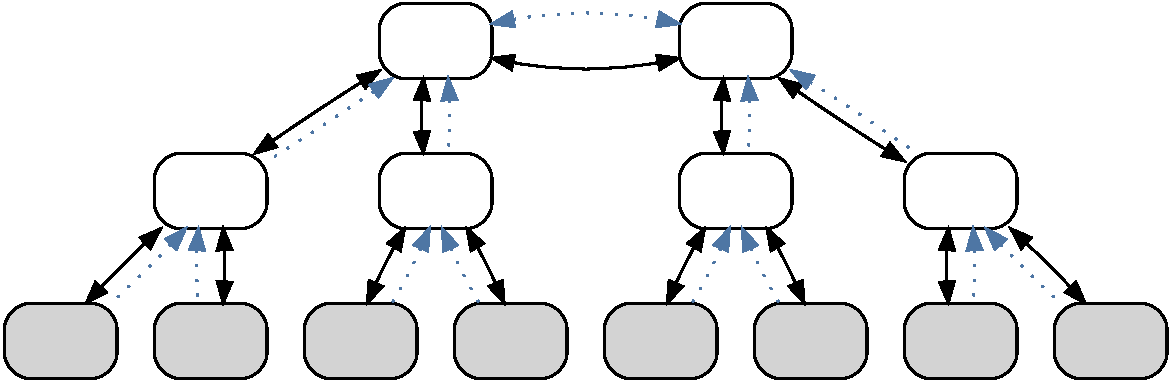
\includegraphics[width=0.2\textwidth]{resources/images/example3}
% \end{wrapfigure}

% \sidenote{Overview}
% \todomid{write about \Cref{fig:req:details}}

% \begin{figure}[H]
%     \centering
%     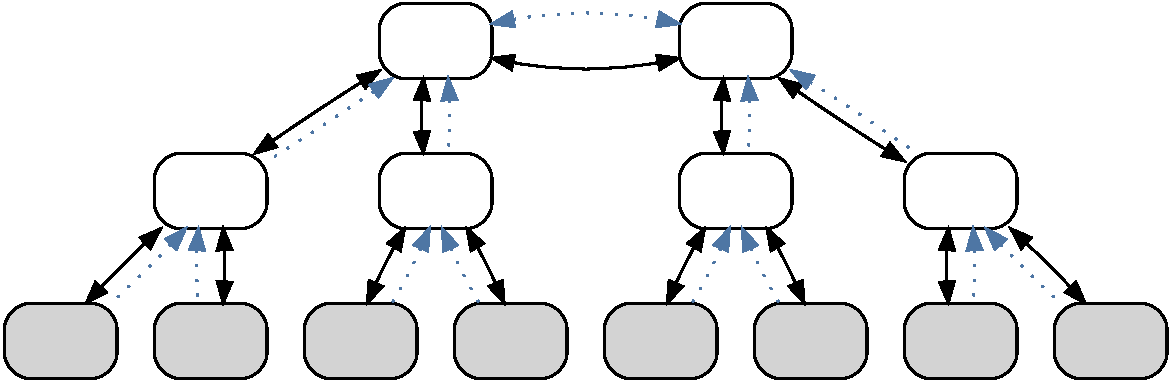
\includegraphics[width=.85\textwidth]{resources/images/example3}
%     \caption{More detailed overview of the requirements}\label{fig:req:details}
% \end{figure}

% \sidenote{Structure of Research}
% \todomid{write about \Cref{fig:hourglass:reqs}}

% \begin{figure}[H]
%     \centering
%     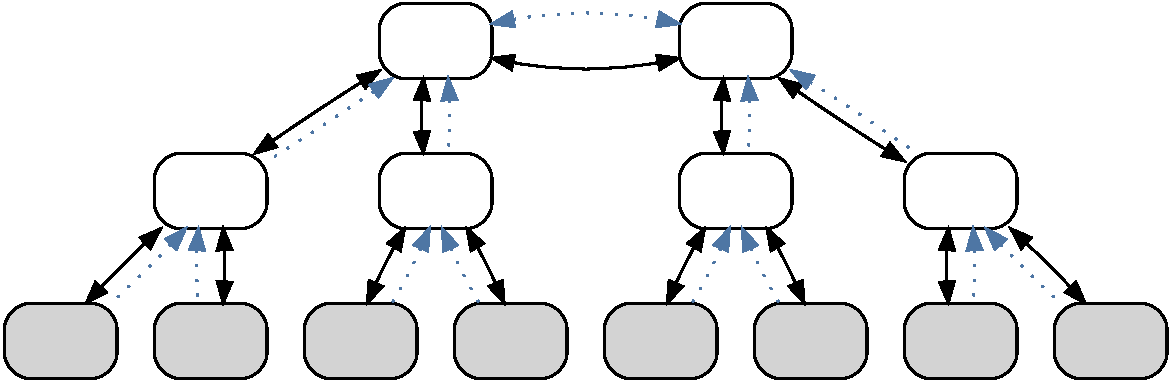
\includegraphics[width=.55\textwidth]{resources/images/example3}
%     \caption{Placement of the requirement section in the structure of research}\label{fig:hourglass:reqs}
% \end{figure}

% \section{Stakeholder 1}

% \sidenote{\Cref{tbl:reqs:stakeholder1}}
% \todomid{write about \Cref{tbl:reqs:stakeholder1}}

% \begin{tabularx}{\textwidth}{lX}
%     \caption{Requirements from stakeholder 1 perspective}\label{tbl:reqs:stakeholder1}\\
%     \toprule
%     \textbf{\#}& \textbf{Description}  \\\midrule
%     \endfirsthead%
%     \toprule
%     \textbf{\#}& \textbf{Description}  \\\midrule
%     \endhead%
%     \requirement{U}{req:stakeholder1:foo}{Foo}
%        & \todomid{write}
%     \\\midrule
%     \requirement{U}{req:stakeholder1:bar}{Bar}
%        & \todomid{write}
%     \\\bottomrule
% \end{tabularx}

% \section{Stakeholder 2}

% \sidenote{\Cref{tbl:reqs:stakeholder2}}
% \todomid{write about \Cref{tbl:reqs:stakeholder2}}

% \begin{tabularx}{\textwidth}{lX}
%     \caption{Requirements from stakeholder 2 perspective}\label{tbl:reqs:stakeholder2}\\
%     \toprule
%     \textbf{\#}& \textbf{Description}  \\\midrule
%     \endfirsthead%
%     \toprule
%     \textbf{\#}& \textbf{Description}  \\\midrule
%     \endhead%
%     \requirement{S}{req:stakeholder2:foo}{Foo}
%        & \todomid{write}
%     \\\midrule
%     \requirement{S}{req:stakeholder2:bar}{Bar}
%        & \todomid{write}
%     \\\bottomrule
% \end{tabularx}

% \section{Stakeholder 3}

% \sidenote{\Cref{tbl:reqs:stakeholder3}}
% \todomid{write about \Cref{tbl:reqs:stakeholder3}}

% \begin{tabularx}{\textwidth}{lX}
%     \caption{Requirements from stakeholder 3 perspective}\label{tbl:reqs:stakeholder3}\\
%     \toprule
%     \textbf{\#}& \textbf{Description}  \\\midrule
%     \endfirsthead%
%     \toprule
%     \textbf{\#}& \textbf{Description}  \\\midrule
%     \endhead%
%     \requirement{T}{req:stakeholder3:foo}{Foo}
%        & \todomid{write}
%     \\\midrule
%     \requirement{T}{req:stakeholder3:bar}{Bar}
%        & \todomid{write}
%     \\\bottomrule
% \end{tabularx}

% \section{Conclusion}

% \sidenote{Summary}
% \todomid{write}

% \sidenote{Takeaway 1}
% \todomid{write}

% \sidenote{Takeaway 2}
% \todomid{write}

% \sidenote{Takeaway 3}
% \todomid{write}

% \sidenote{Next chapter}
% \todomid{write}

    % \cleardoublepage
\chapter{Plan and Timeline}\minitoc\label{sec:plan}\vspace{.5cm}

This chapter will outline our project plan and provide a timeline for its execution.

\section{Project Plan}

\begin{figure}[H]
	\centering
	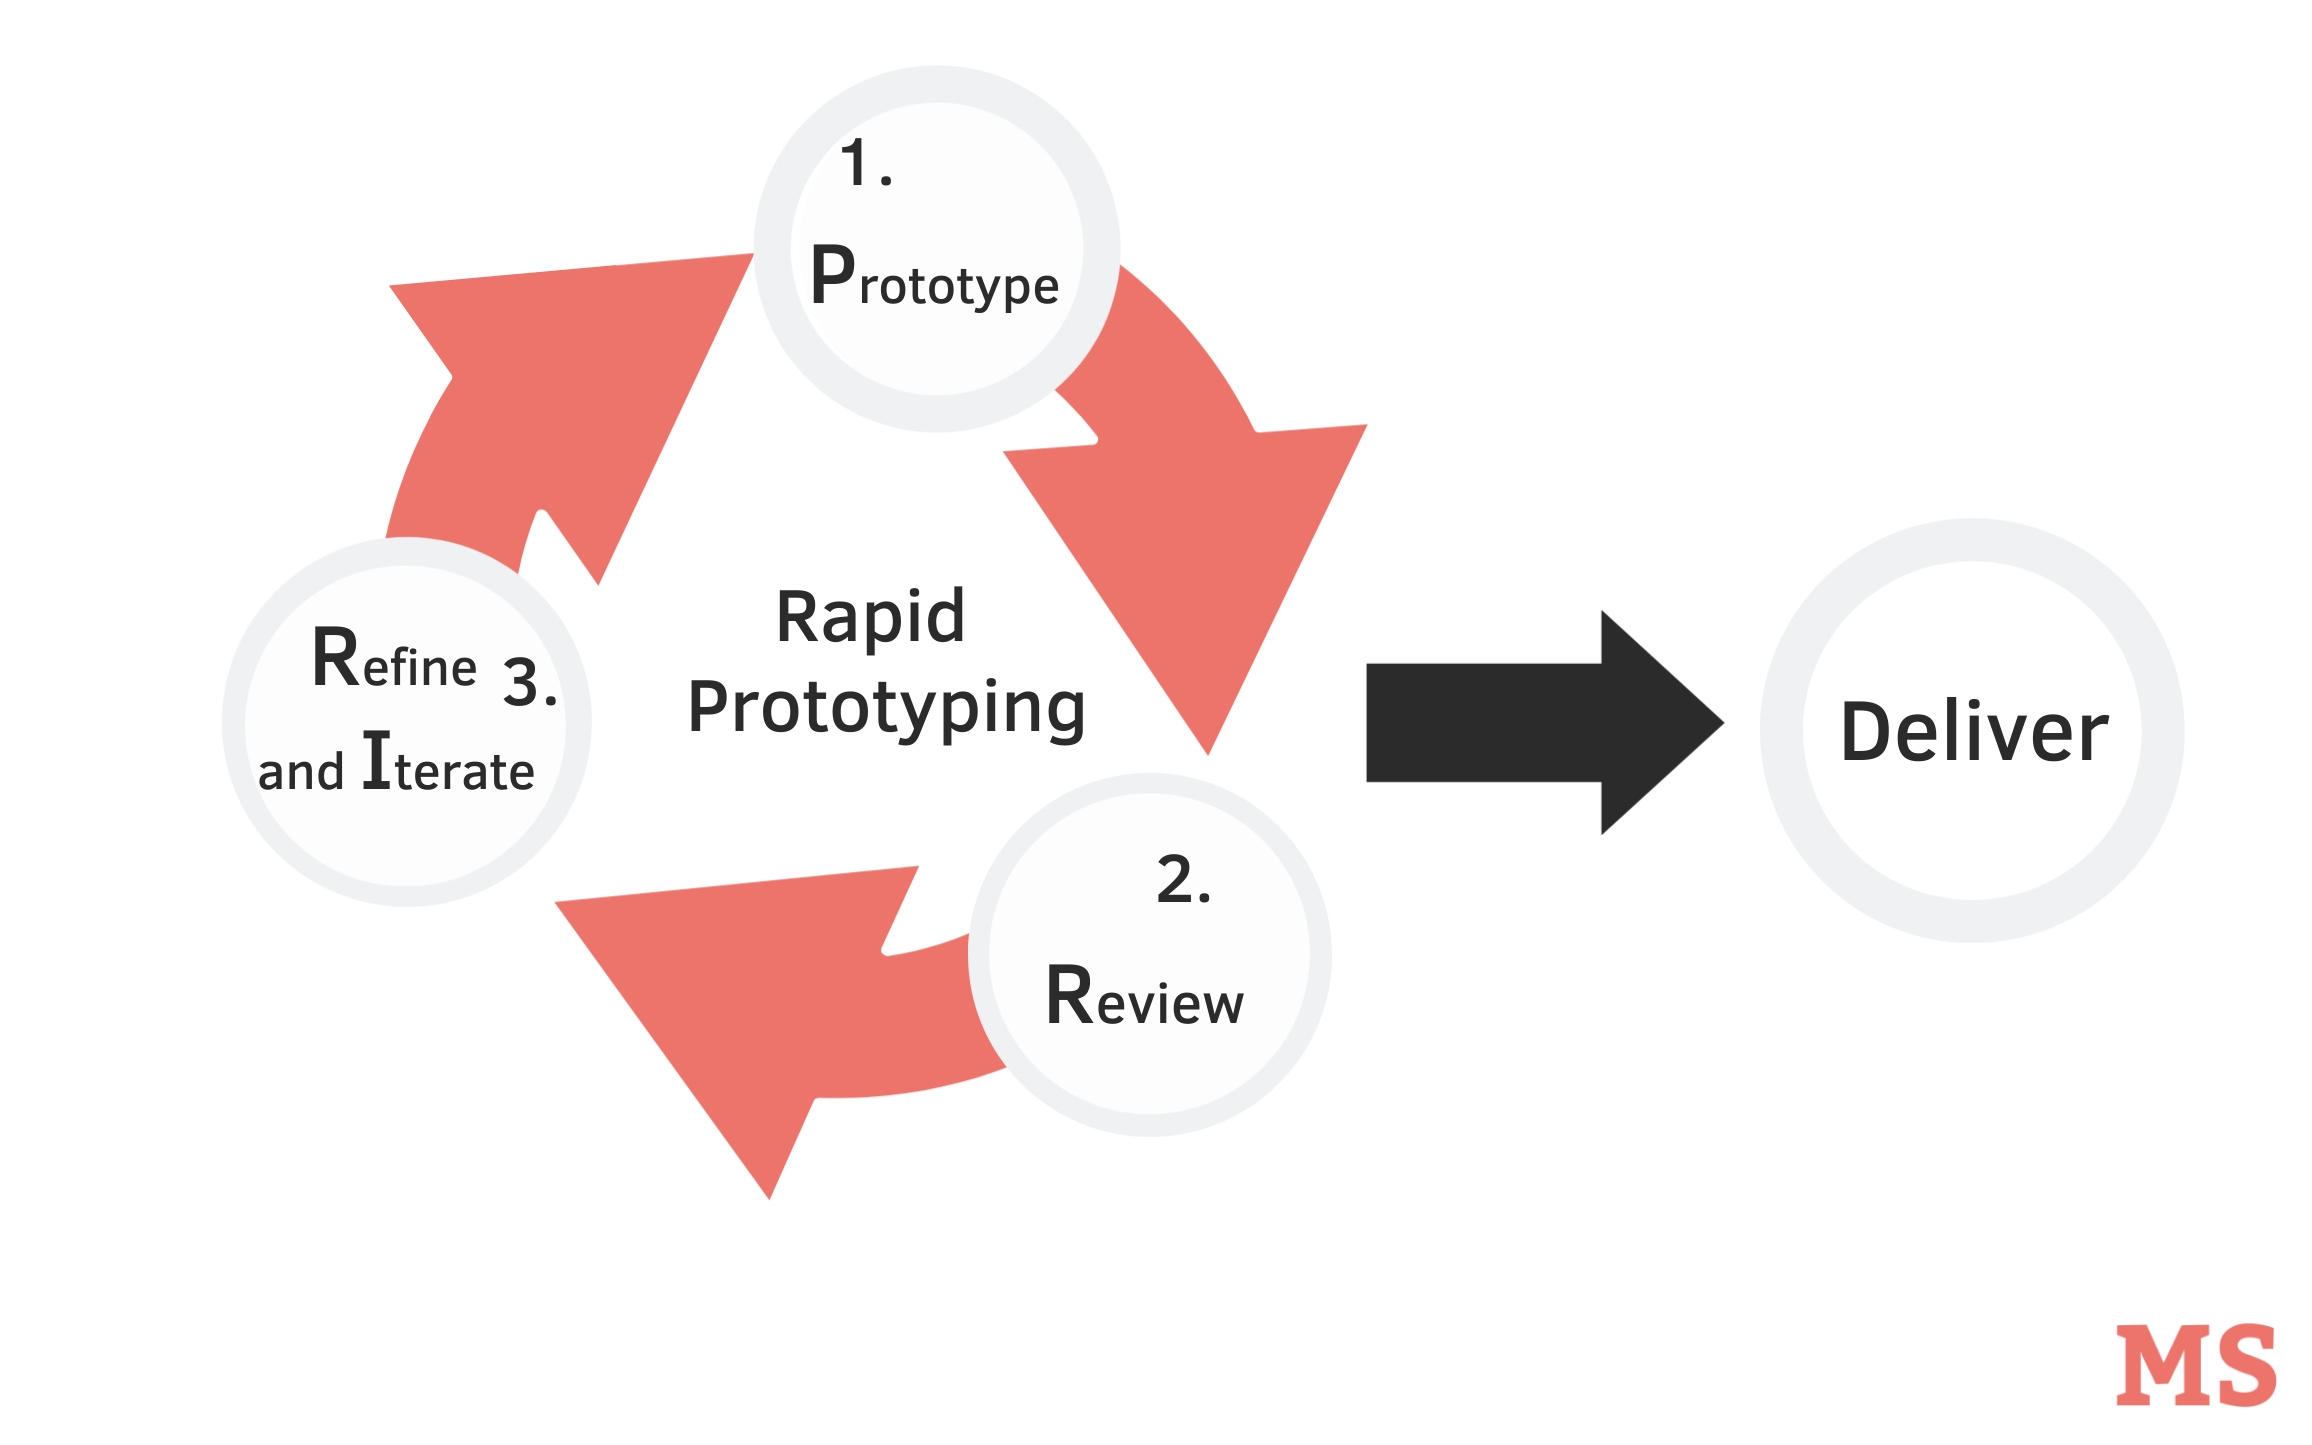
\includegraphics[width=0.6\textwidth]{rapid_prototyping_software.png}
	\caption{Rapid prototyping cycle \cite{marketsplash_rapid_2021}}
	\label{fig:plan:rapid_prototyping_software}
\end{figure}

During the development phase, we adhere to the rapid prototyping model (\Cref{fig:plan:rapid_prototyping_software}). 
The development process follows a loop of building prototypes, reviewing them, refining the implementation, and iterating on the design. 
Features and components are broken into  self-contained and independent tasks, each can be completed within a time frame of 1-2 weeks.
\\


The thesis is set to be completed in 6 months (\Cref{fig:plan:TIMELINE}), divided in 3 phases: \textbf{Prototype Building}, \textbf{Feature}, and \textbf{Refinary and Test}.
The library's development is expected to span a period of 3 months. 
During the initial month, the focus will be on creating the core features of MTX. 
These features involve tasks such as packet exchange with XDP socket, collecting and delivering packets from applications, and inspecting packets for flow control purposes. 
The subsequent 4 weeks will be dedicated to refactoring and shaping the library, ensuring it meets the necessary requirements for packaging and distribution. 
Following this, the third month will be allocated to constructing the control and data plane to support various configurations. 
After completing the development process, the fourth month will primarily involve testing the library and addressing any issues that may arise. 
The remaining two months will be used for building a test application, conducting thorough testing, and analyzing the obtained data. 
Throughout the entire development process, updates will be made to the thesis documentation.


\clearpage
\begin{sidewaysfigure}
    \centering
    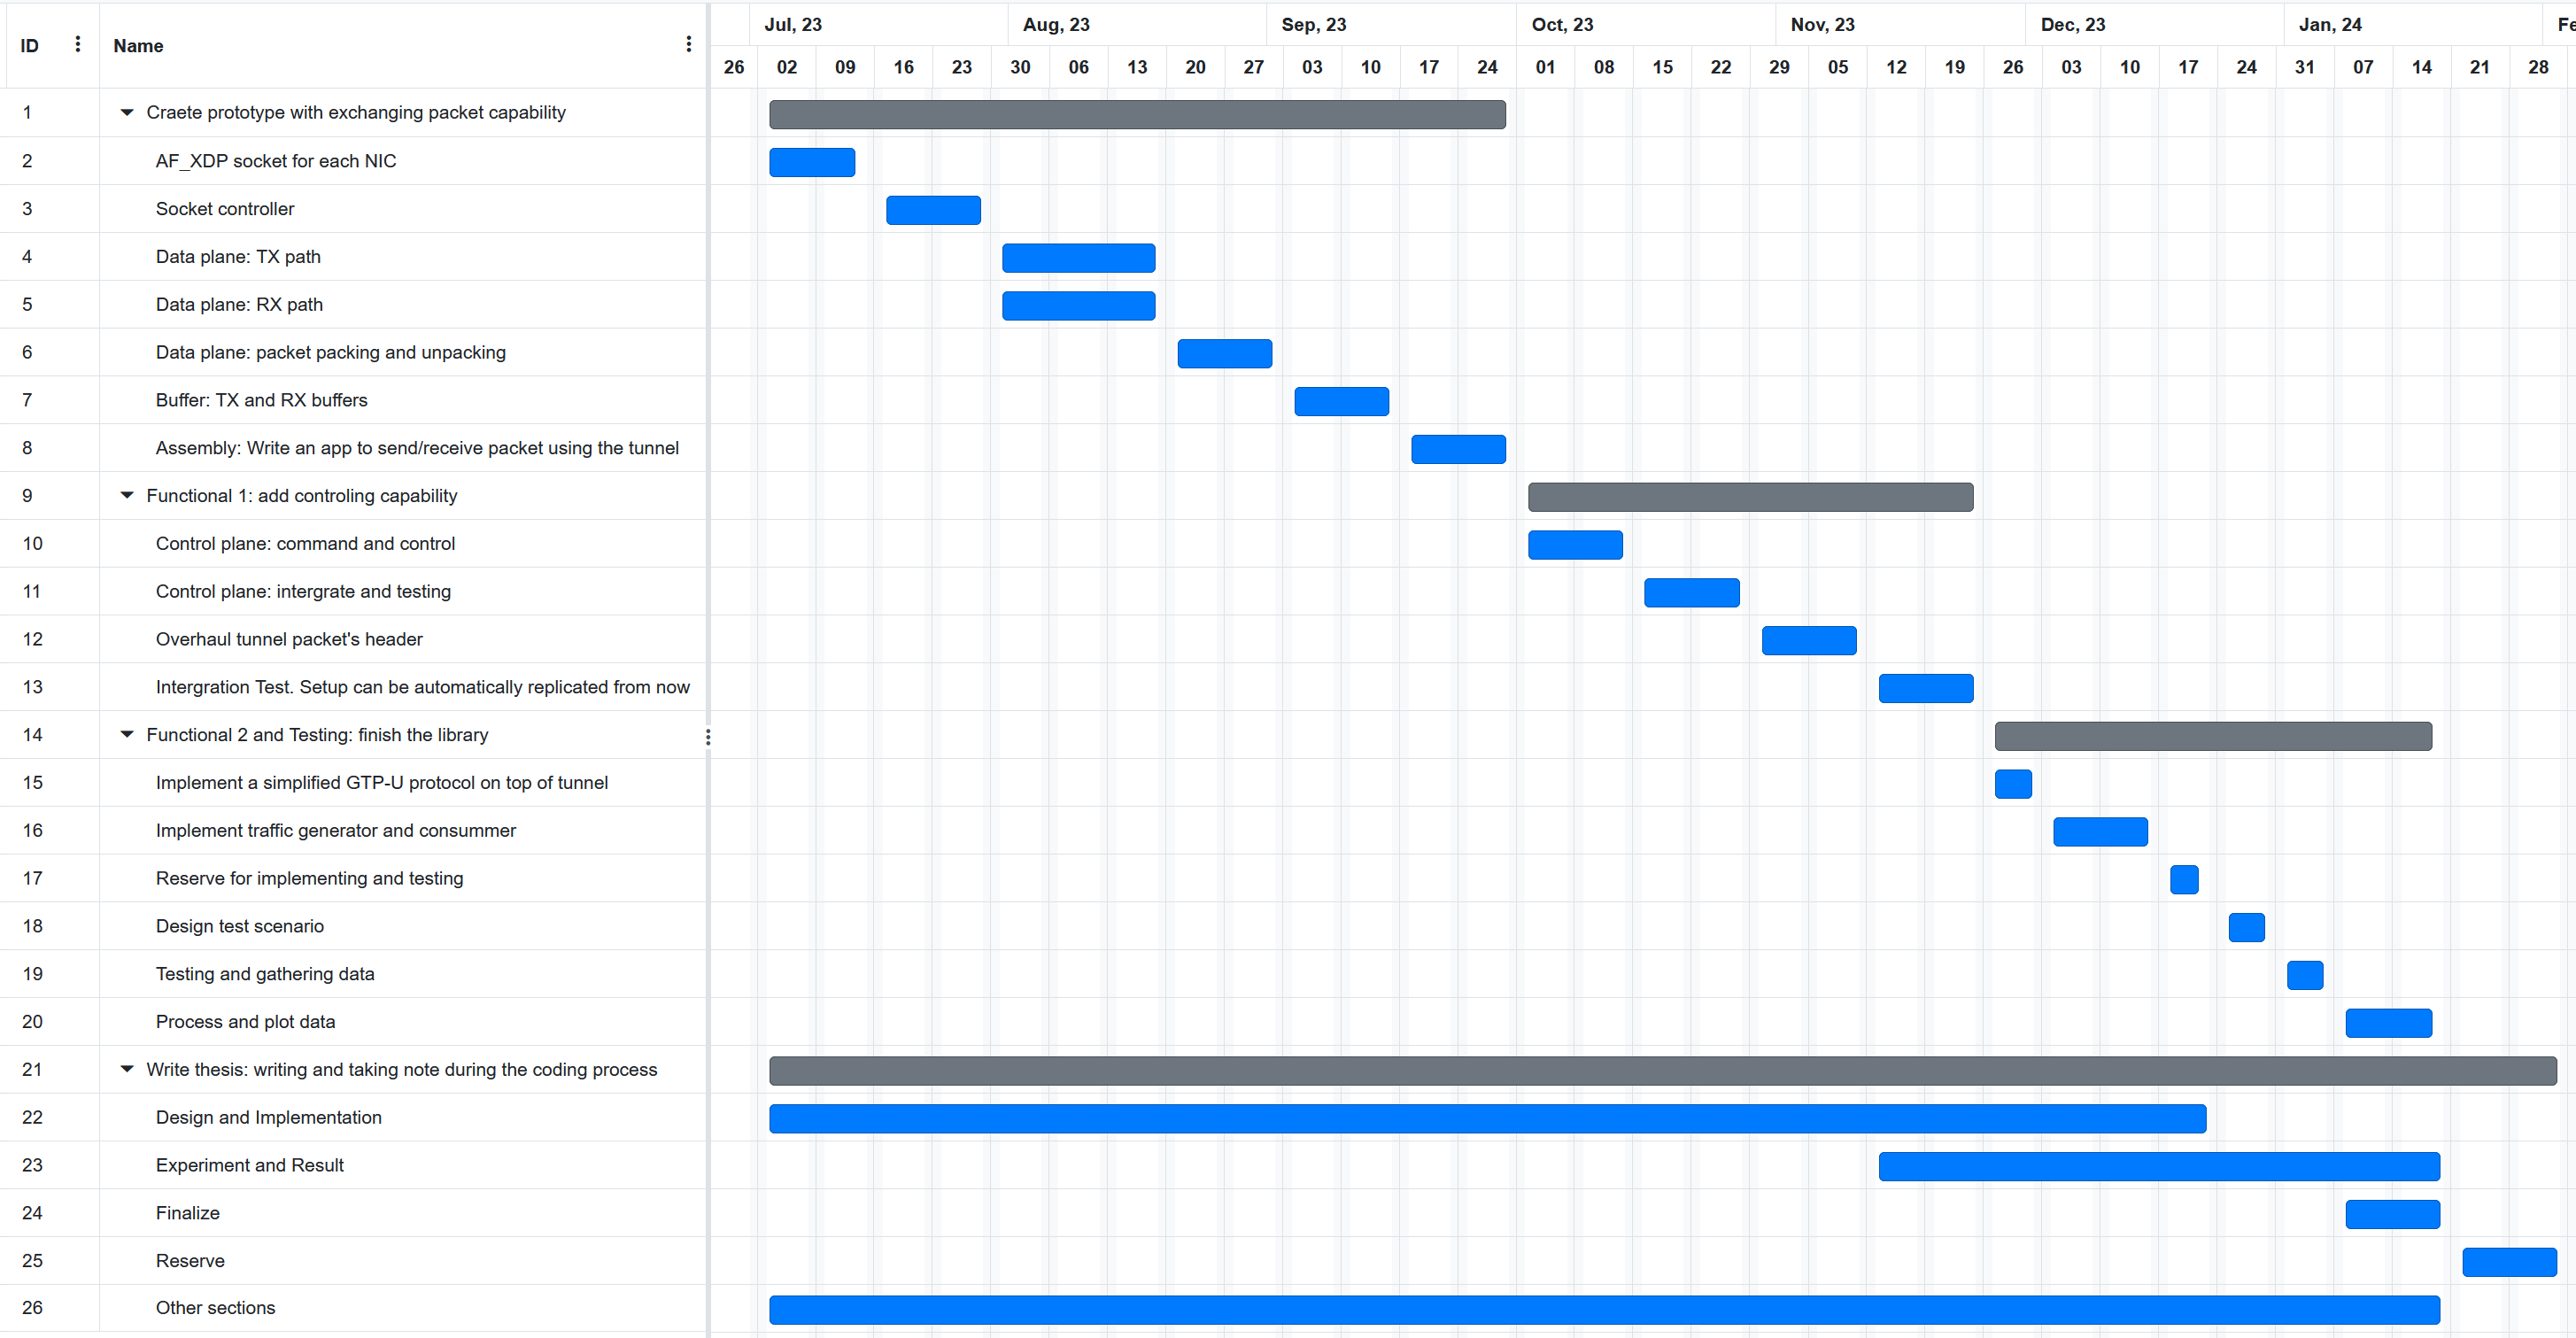
\includegraphics[width=1.0\textwidth]{resources/images/TIMELINE.PNG}
    \caption{Expected progress for the thesis project}
	\label{fig:plan:TIMELINE}
  \end{sidewaysfigure}

\clearpage
\section{Development Environment}
The development process will take place within a Linux environment. 
As for testing purposes, the program binary will be deployed and executed on 2 industrial-grade computers \textit{UP CORE} designed by \ac{AAEON}, equipped with multiple Ethernet ports \cite{upc_core} \cite{upc_extension_board}. 
The binary will establish a tunnel between two UPC machines using three specific Ethernet ports. 
It's important to note that the fourth port is unrelated to the multipath tunneling and is solely used for remote management purposes.
The UPC machines, equipped with this library, can be utilized as part of the AV's 5G test bed. 
In this setup, RAN (Radio Access Network) and Open5GS software will be installed on the UPC machines, enabling comprehensive testing and evaluation of 5G functionalities.

\begin{figure}[H]
	\centering
	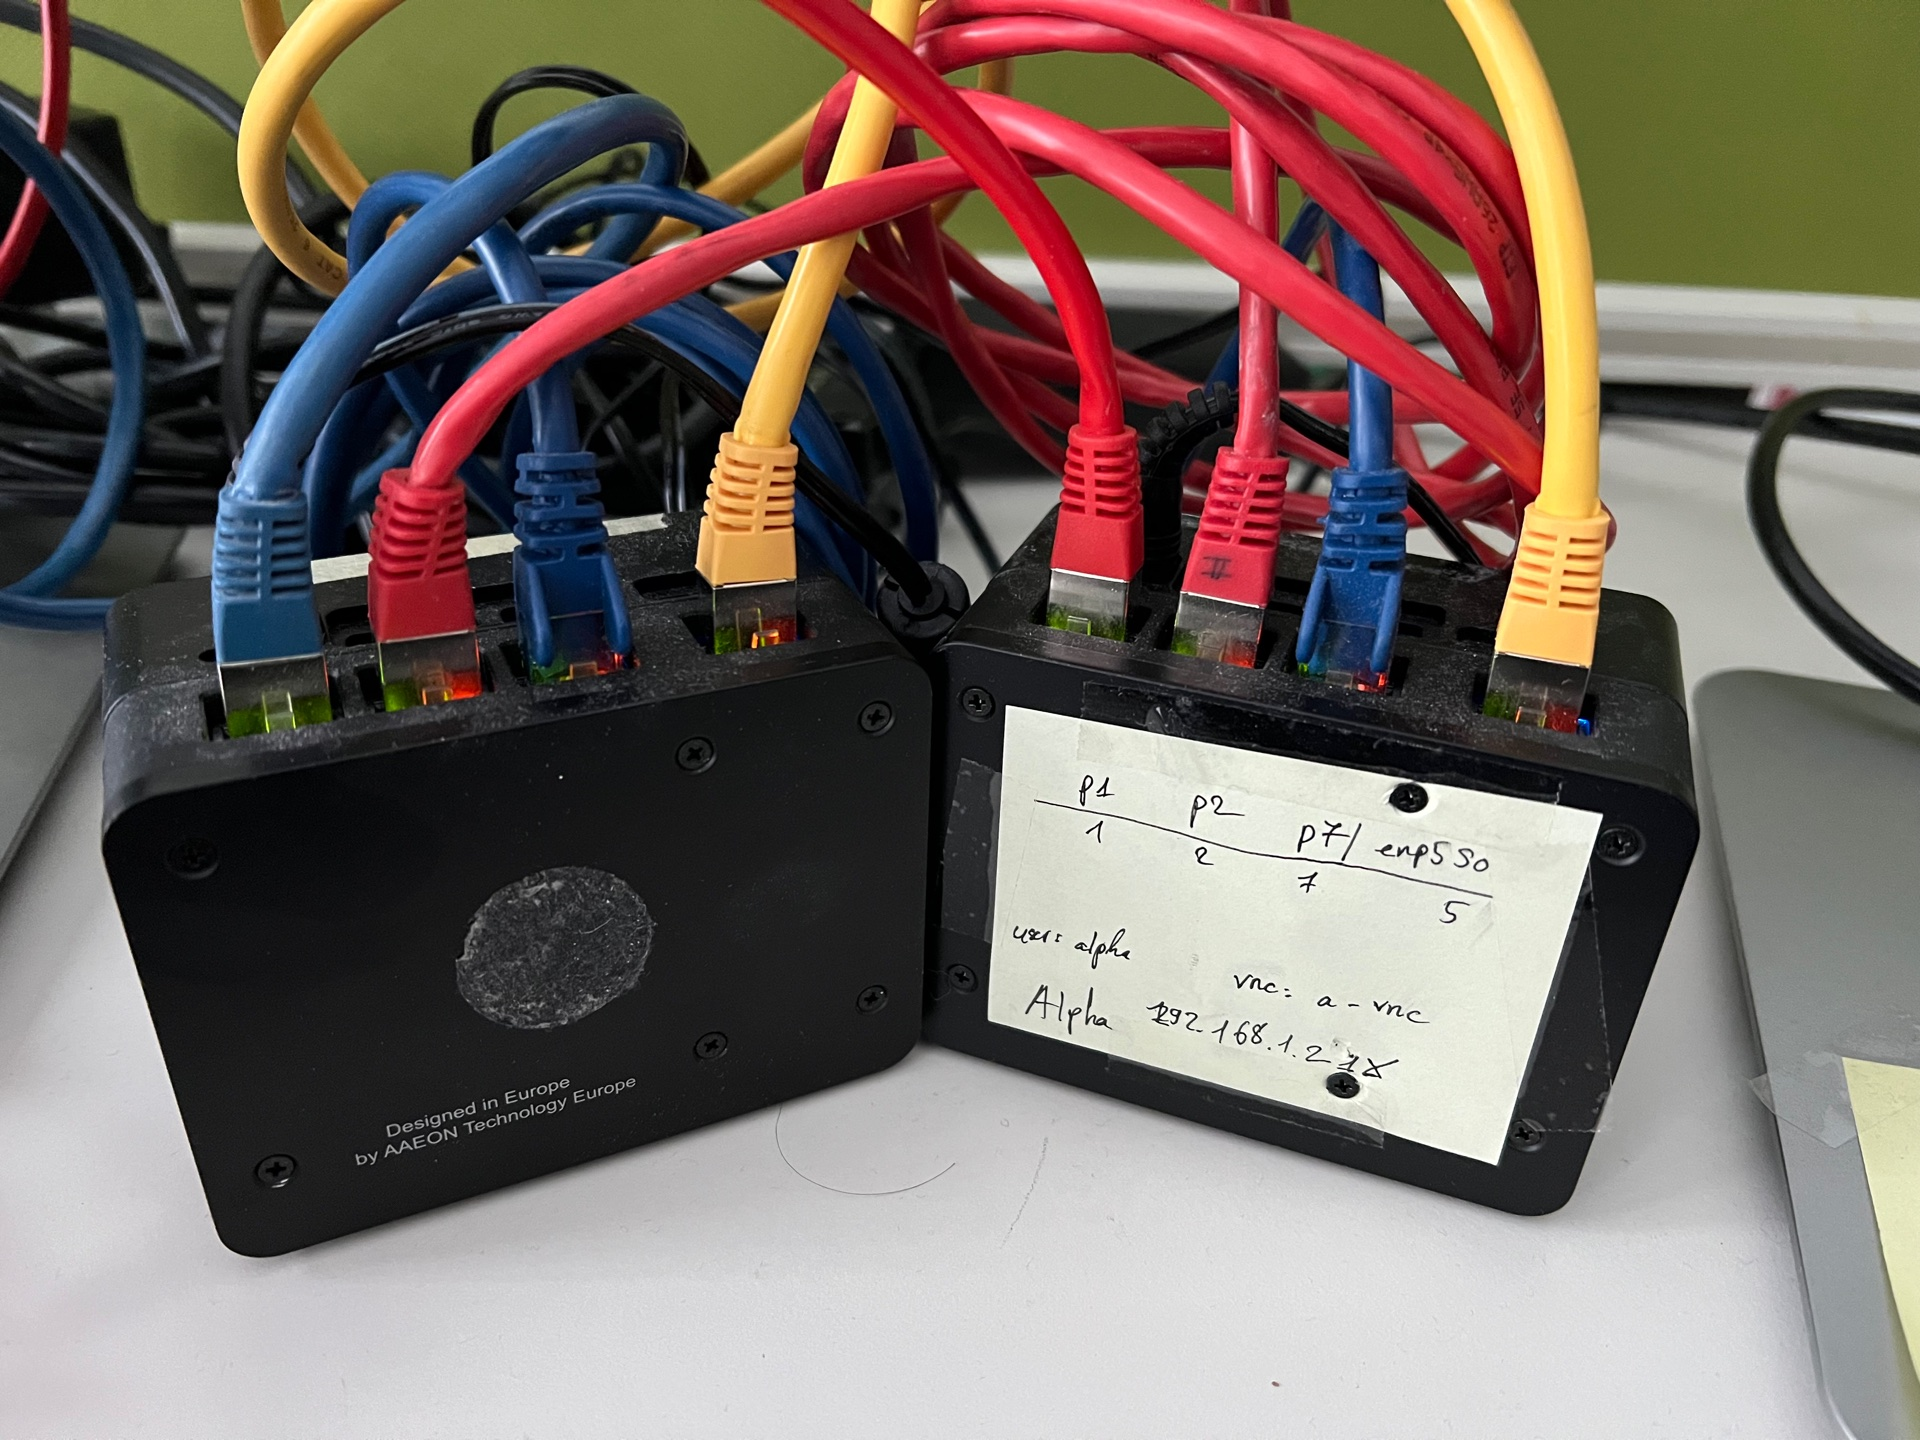
\includegraphics[width=0.8\textwidth]{upc_machines.png}
	\caption{Two UPC machines with 3 ethernet ports connected (\textit{enp3s0}, \textit{enp5s0}, \textit{enp7s0}). Port \textit{enp1s0} is connected to workstation for remote management purpose.}
	\label{fig:plan:upc_machines}
\end{figure}

    % \cleardoublepage
\chapter{Contribution 1}\label{sec:contrib1}\minitoc\vspace{.5cm}
\index{Contribution 1}

\section{Introduction}

\begin{wrapfigure}{r}{0.2\textwidth}
    \centering
    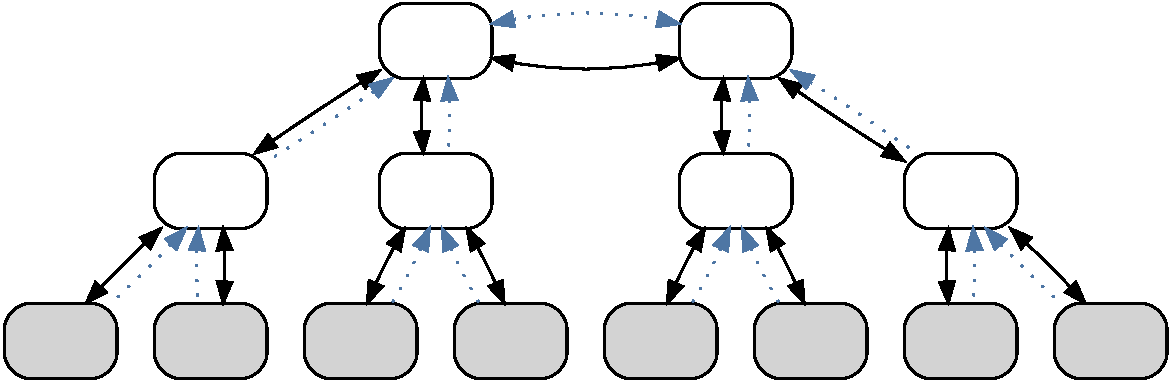
\includegraphics[width=0.2\textwidth]{resources/images/example3}
\end{wrapfigure}

\sidenote{Overview}
\todomid{write}

\sidenote{Structure of Research}
\todomid{write about \Cref{fig:hourglass:contrib1}}

\begin{figure}[H]
    \centering
    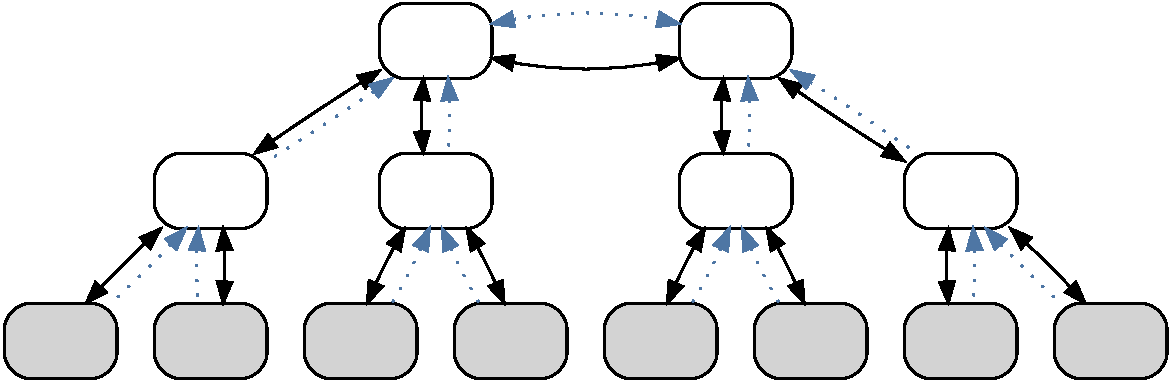
\includegraphics[width=.55\textwidth]{resources/images/example3}
    \caption{Placement of contribution 1 in the structure of research}\label{fig:hourglass:contrib1}
\end{figure}

\section{State of the Art}

\sidenote{Overview}
\todomid{write about \Cref{fig:contrib1:related}}

\begin{figure}[htbp]
    \centering
    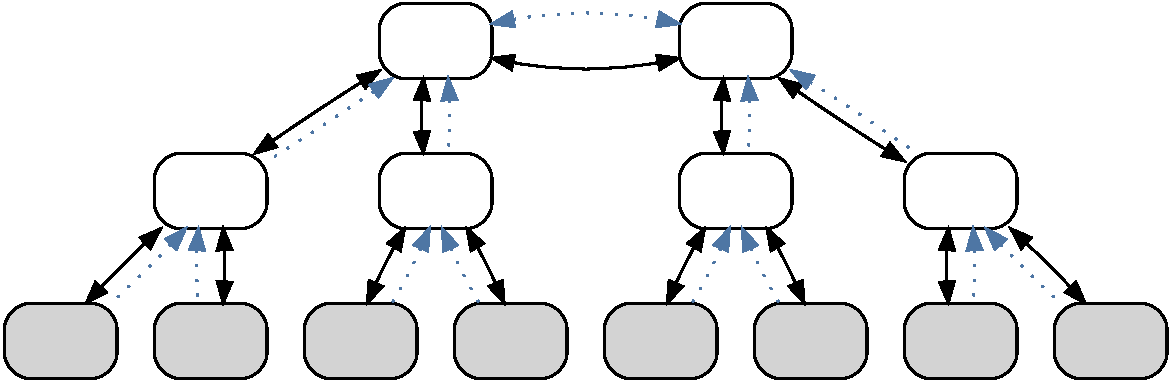
\includegraphics[width=.6\textwidth]{resources/images/example3}
    \caption{Relationship of contribution 1 to related work}\label{fig:contrib1:related}
\end{figure}

\subsection{Related Work 1}

\sidenote{Overview}
\todomid{write}

\sidenote{Some Aspects}
\todomid{write}

\sidenote{Issues}
\todomid{write about \Cref{lst:contrib1:rw1}}

\lstset{caption=Listing related to related work 1 for contribution 1, label=lst:contrib1:rw1,
language=xml, breaklines=true, numbers=left, basicstyle=\small\ttfamily,
stepnumber=1, frame=single, inputencoding=utf8/latin1}~\lstinputlisting{resources/code/example.java}

\subsection{Related Work 2}

\sidenote{Overview}
\todomid{write}

\sidenote{Some Aspects}
\todomid{write}

\sidenote{Issues}
\todomid{write about \Cref{lst:contrib1:rw2}}

\lstset{caption=Listing related to related work 2 for contribution 1, label=lst:contrib1:rw2,
language=xml, breaklines=true, numbers=left, basicstyle=\small\ttfamily,
stepnumber=1, frame=single, inputencoding=utf8/latin1}~\lstinputlisting{resources/code/example.java}

\subsection{Related Work 3}

\sidenote{Overview}
\todomid{write}

\sidenote{Some Aspects}
\todomid{write}

\sidenote{Issues}
\todomid{write about \Cref{lst:contrib1:rw3}}

\lstset{caption=Listing related to related work 3 for contribution 1, label=lst:contrib1:rw3,
language=xml, breaklines=true, numbers=left, basicstyle=\small\ttfamily,
stepnumber=1, frame=single, inputencoding=utf8/latin1}~\lstinputlisting{resources/code/example.java}


\section{Own Approach}

\subsection{Overview}

\sidenote{Intro}
\todomid{write}

\sidenote{Goal}
\todomid{write about \Cref{fig:contrib1:goal}}

\begin{figure}[htbp]
    \centering
    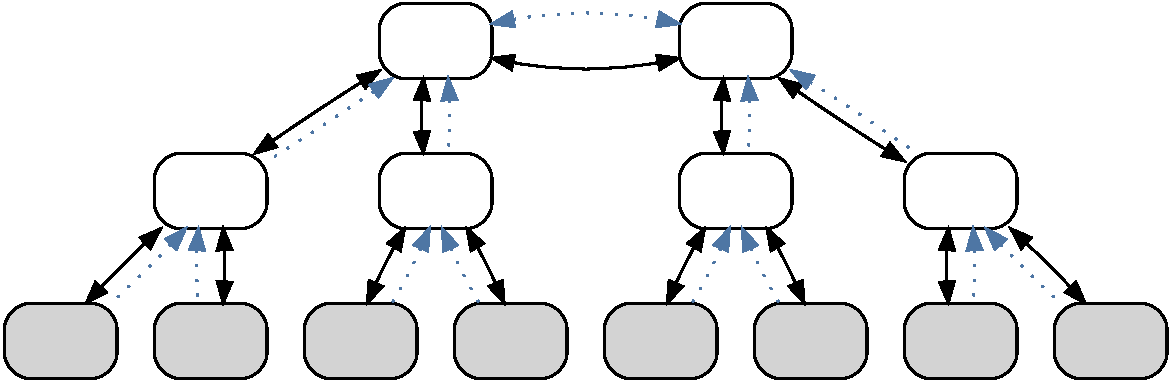
\includegraphics[width=.95\textwidth]{resources/images/example3}
    \caption{Contribution 1 goal}\label{fig:contrib1:goal}
\end{figure}

\sidenote{Approach}
\todomid{write}

\subsection{First Part}

\sidenote{Overview}
\todomid{write}

\sidenote{Approach}
\todomid{write}

\sidenote{Integration}
\todomid{write}

\subsection{Second Part}

\sidenote{Overview}
\todomid{write}

\sidenote{Approach}
\todomid{write}

\sidenote{Integration}
\todomid{write}

\subsection{Third Part}

\sidenote{Overview}
\todomid{write}

\sidenote{Approach}
\todomid{write}

\sidenote{Integration}
\todomid{write}

\section{Conclusion}

\sidenote{Summary}
\todomid{write}

\sidenote{Takeaway 1}
\todomid{write}

\sidenote{Takeaway 2}
\todomid{write}

\sidenote{Takeaway 3}
\todomid{write}

\sidenote{Next chapter}
\todomid{write}

    % \cleardoublepage
\chapter{Contribution 2}\label{sec:contrib2}\minitoc\vspace{.5cm}
\index{Contribution 2}

\section{Introduction}

\begin{wrapfigure}{r}{0.2\textwidth}
    \centering
    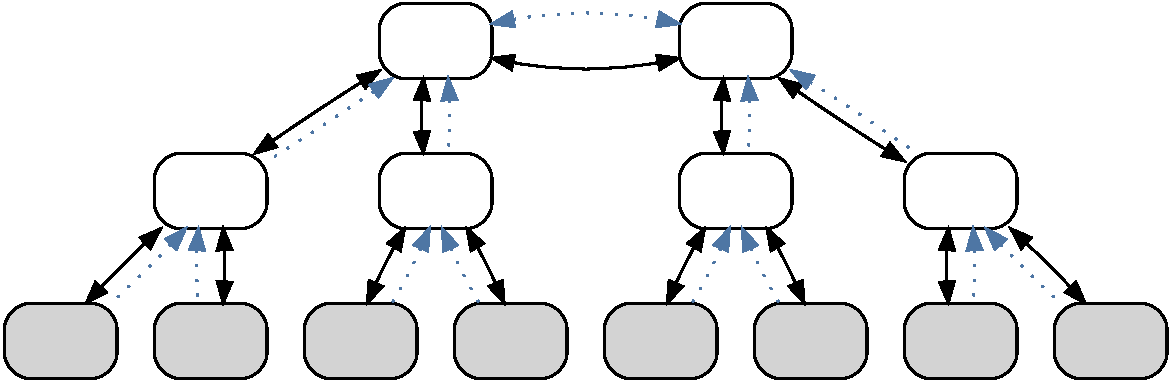
\includegraphics[width=0.2\textwidth]{resources/images/example3}
\end{wrapfigure}

\sidenote{Overview}
\todomid{write}

\sidenote{Structure of Research}
\todomid{write about \Cref{fig:hourglass:contrib2}}

\begin{figure}[H]
    \centering
    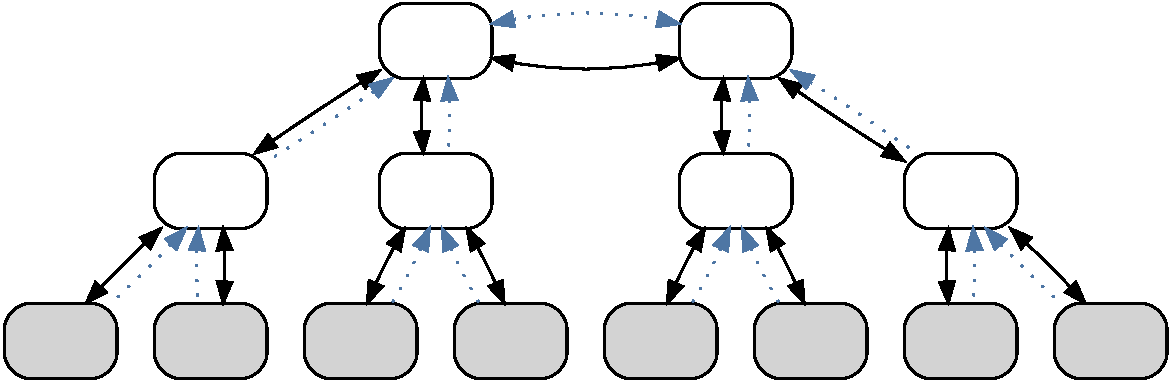
\includegraphics[width=.55\textwidth]{resources/images/example3}
    \caption{Placement of Contribution 2 in the structure of research}\label{fig:hourglass:contrib2}
\end{figure}

\section{State of the Art}

\sidenote{Overview}
\todomid{write about \Cref{fig:contrib2:related}}

\begin{figure}[htbp]
    \centering
    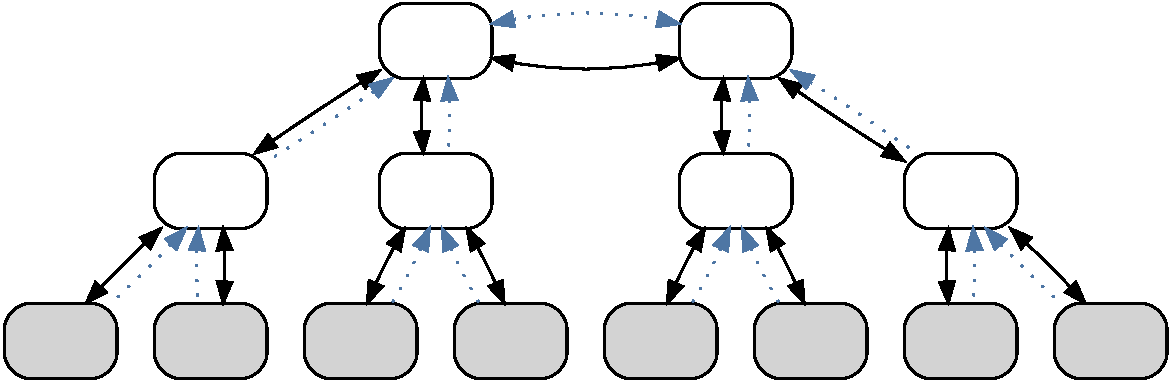
\includegraphics[width=.6\textwidth]{resources/images/example3}
    \caption{Relationship of Contribution 2 to related work}\label{fig:contrib2:related}
\end{figure}

\subsection{Related Work 1}

\sidenote{Overview}
\todomid{write}

\sidenote{Some Aspects}
\todomid{write}

\sidenote{Issues}
\todomid{write about \Cref{lst:contrib2:rw1}}

\lstset{caption=Listing related to related work 1 for Contribution 2, label=lst:contrib2:rw1,
language=xml, breaklines=true, numbers=left, basicstyle=\small\ttfamily,
stepnumber=1, frame=single, inputencoding=utf8/latin1}~\lstinputlisting{resources/code/example.java}

\subsection{Related Work 2}

\sidenote{Overview}
\todomid{write}

\sidenote{Some Aspects}
\todomid{write}

\sidenote{Issues}
\todomid{write about \Cref{lst:contrib2:rw2}}

\lstset{caption=Listing related to related work 2 for Contribution 2, label=lst:contrib2:rw2,
language=xml, breaklines=true, numbers=left, basicstyle=\small\ttfamily,
stepnumber=1, frame=single, inputencoding=utf8/latin1}~\lstinputlisting{resources/code/example.java}

\subsection{Related Work 3}

\sidenote{Overview}
\todomid{write}

\sidenote{Some Aspects}
\todomid{write}

\sidenote{Issues}
\todomid{write about \Cref{lst:contrib2:rw3}}

\lstset{caption=Listing related to related work 3 for Contribution 2, label=lst:contrib2:rw3,
language=xml, breaklines=true, numbers=left, basicstyle=\small\ttfamily,
stepnumber=1, frame=single, inputencoding=utf8/latin1}~\lstinputlisting{resources/code/example.java}


\section{Own Approach}

\subsection{Overview}

\sidenote{Intro}
\todomid{write}

\sidenote{Goal}
\todomid{write about \Cref{fig:contrib2:goal}}

\begin{figure}[htbp]
    \centering
    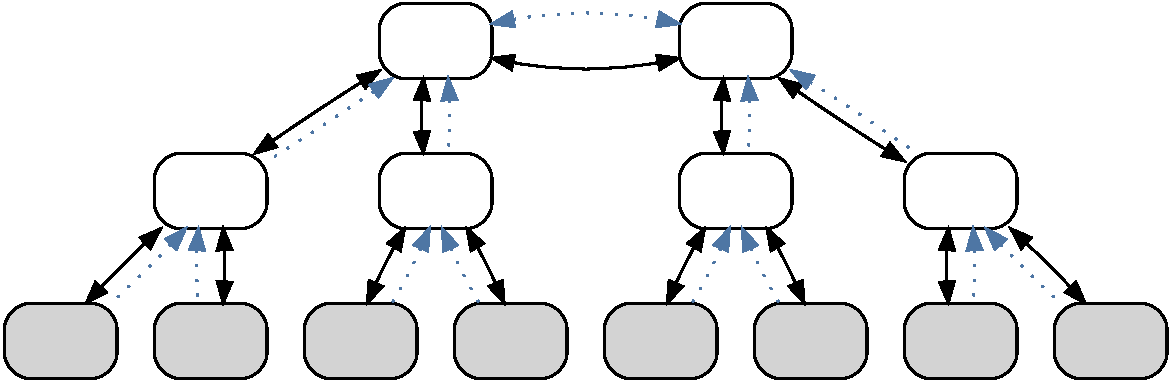
\includegraphics[width=.95\textwidth]{resources/images/example3}
    \caption{Contribution 2 goal}\label{fig:contrib2:goal}
\end{figure}

\sidenote{Approach}
\todomid{write}

\subsection{First Part}

\sidenote{Overview}
\todomid{write}

\sidenote{Approach}
\todomid{write}

\sidenote{Integration}
\todomid{write}

\subsection{Second Part}

\sidenote{Overview}
\todomid{write}

\sidenote{Approach}
\todomid{write}

\sidenote{Integration}
\todomid{write}

\subsection{Third Part}

\sidenote{Overview}
\todomid{write}

\sidenote{Approach}
\todomid{write}

\sidenote{Integration}
\todomid{write}

\section{Conclusion}

\sidenote{Summary}
\todomid{write}

\sidenote{Takeaway 1}
\todomid{write}

\sidenote{Takeaway 2}
\todomid{write}

\sidenote{Takeaway 3}
\todomid{write}

\sidenote{Next chapter}
\todomid{write}

    % % \cleardoublepage
\chapter{Contribution 3}\label{sec:contrib3}\minitoc\vspace{.5cm}
\index{Contribution 3}

\section{Introduction}

\begin{wrapfigure}{r}{0.2\textwidth}
    \centering
    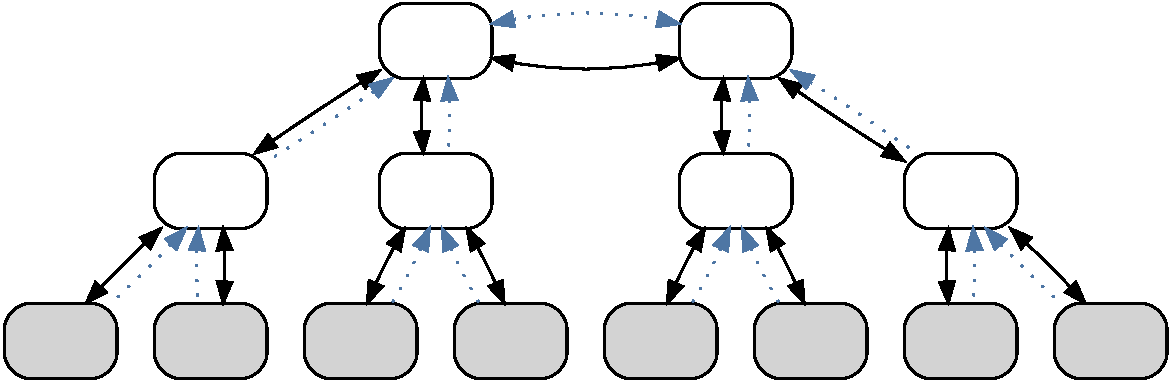
\includegraphics[width=0.2\textwidth]{resources/images/example3}
\end{wrapfigure}

\sidenote{Overview}
\todomid{write}

\sidenote{Structure of Research}
\todomid{write about \Cref{fig:hourglass:contrib3}}

\begin{figure}[H]
    \centering
    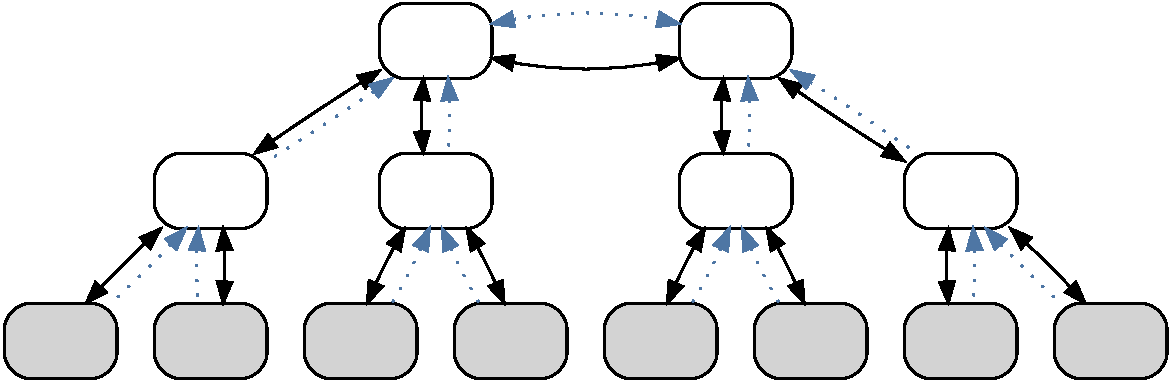
\includegraphics[width=.55\textwidth]{resources/images/example3}
    \caption{Placement of Contribution 3 in the structure of research}\label{fig:hourglass:contrib3}
\end{figure}

\section{State of the Art}

\sidenote{Overview}
\todomid{write about \Cref{fig:contrib3:related}}

\begin{figure}[htbp]
    \centering
    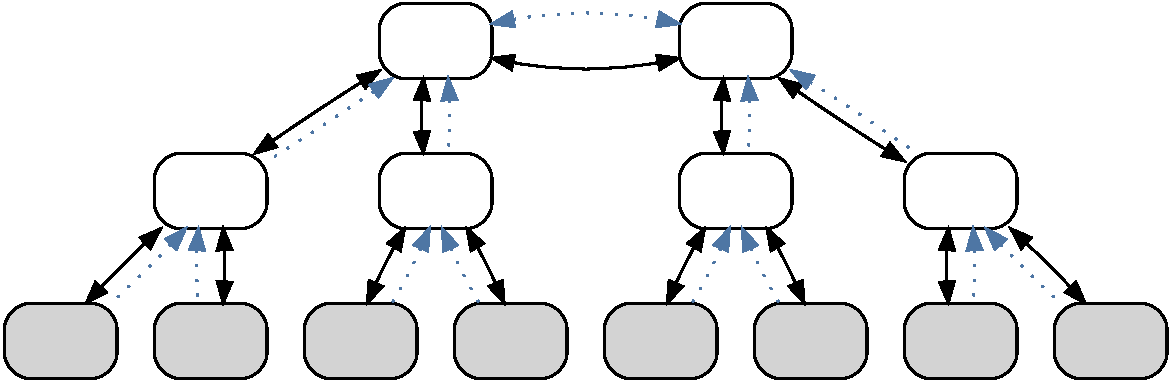
\includegraphics[width=.6\textwidth]{resources/images/example3}
    \caption{Relationship of Contribution 3 to related work}\label{fig:contrib3:related}
\end{figure}

\subsection{Related Work 1}

\sidenote{Overview}
\todomid{write}

\sidenote{Some Aspects}
\todomid{write}

\sidenote{Issues}
\todomid{write about \Cref{lst:contrib3:rw1}}

\lstset{caption=Listing related to related work 1 for Contribution 3, label=lst:contrib3:rw1,
language=xml, breaklines=true, numbers=left, basicstyle=\small\ttfamily,
stepnumber=1, frame=single, inputencoding=utf8/latin1}~\lstinputlisting{resources/code/example.java}

\subsection{Related Work 2}

\sidenote{Overview}
\todomid{write}

\sidenote{Some Aspects}
\todomid{write}

\sidenote{Issues}
\todomid{write about \Cref{lst:contrib3:rw2}}

\lstset{caption=Listing related to related work 2 for Contribution 3, label=lst:contrib3:rw2,
language=xml, breaklines=true, numbers=left, basicstyle=\small\ttfamily,
stepnumber=1, frame=single, inputencoding=utf8/latin1}~\lstinputlisting{resources/code/example.java}

\subsection{Related Work 3}

\sidenote{Overview}
\todomid{write}

\sidenote{Some Aspects}
\todomid{write}

\sidenote{Issues}
\todomid{write about \Cref{lst:contrib3:rw3}}

\lstset{caption=Listing related to related work 3 for Contribution 3, label=lst:contrib3:rw3,
language=xml, breaklines=true, numbers=left, basicstyle=\small\ttfamily,
stepnumber=1, frame=single, inputencoding=utf8/latin1}~\lstinputlisting{resources/code/example.java}


\section{Own Approach}

\subsection{Overview}

\sidenote{Intro}
\todomid{write}

\sidenote{Goal}
\todomid{write about \Cref{fig:contrib3:goal}}

\begin{figure}[htbp]
    \centering
    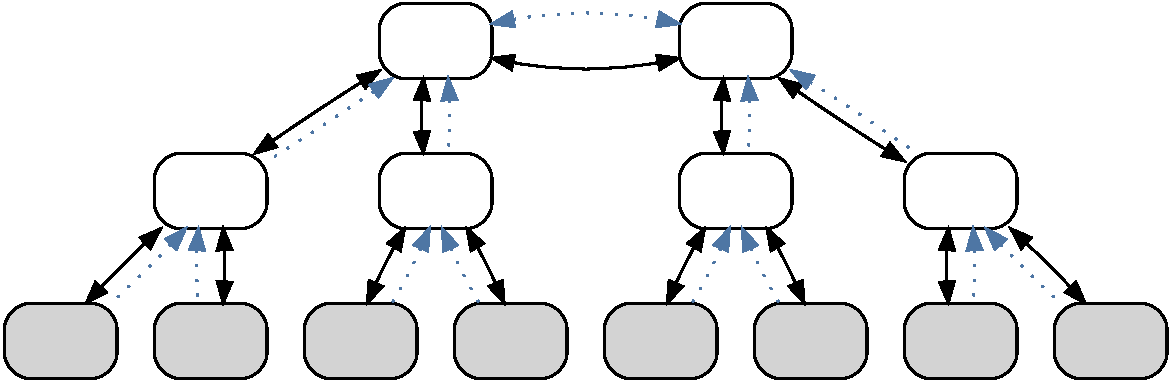
\includegraphics[width=.95\textwidth]{resources/images/example3}
    \caption{Contribution 3 goal}\label{fig:contrib3:goal}
\end{figure}

\sidenote{Approach}
\todomid{write}

\subsection{First Part}

\sidenote{Overview}
\todomid{write}

\sidenote{Approach}
\todomid{write}

\sidenote{Integration}
\todomid{write}

\subsection{Second Part}

\sidenote{Overview}
\todomid{write}

\sidenote{Approach}
\todomid{write}

\sidenote{Integration}
\todomid{write}

\subsection{Third Part}

\sidenote{Overview}
\todomid{write}

\sidenote{Approach}
\todomid{write}

\sidenote{Integration}
\todomid{write}

\section{Conclusion}

\sidenote{Summary}
\todomid{write}

\sidenote{Takeaway 1}
\todomid{write}

\sidenote{Takeaway 2}
\todomid{write}

\sidenote{Takeaway 3}
\todomid{write}

\sidenote{Next chapter}
\todomid{write}

    % % \cleardoublepage
\chapter{Evaluation}\label{sec:eval}\minitoc\vspace{.5cm}
\index{Evaluation}\index{Validation}\index{Verification}

\section{Introduction}

\begin{wrapfigure}{r}{0.2\textwidth}
    \centering
    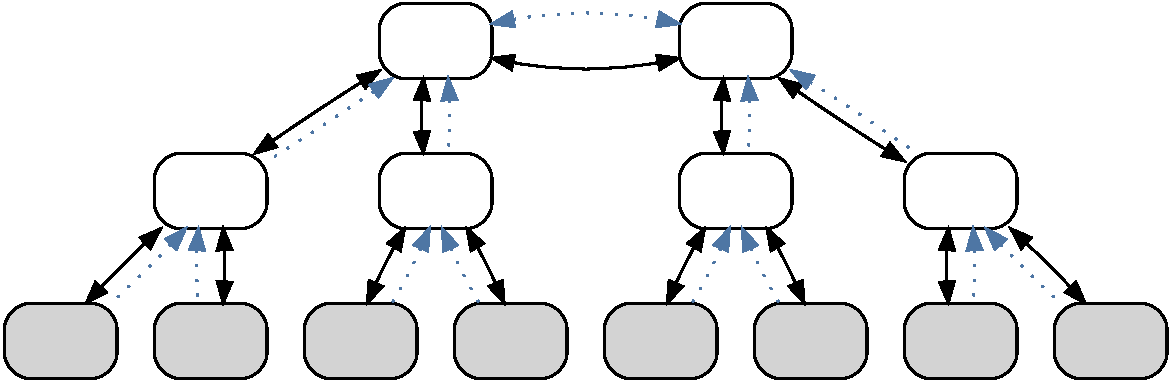
\includegraphics[width=0.2\textwidth]{resources/images/example3}
\end{wrapfigure}

\sidenote{Overview}
\todomid{write about \Cref{sec:eval:tec}}

\begin{figure}[htbp]
    \centering
    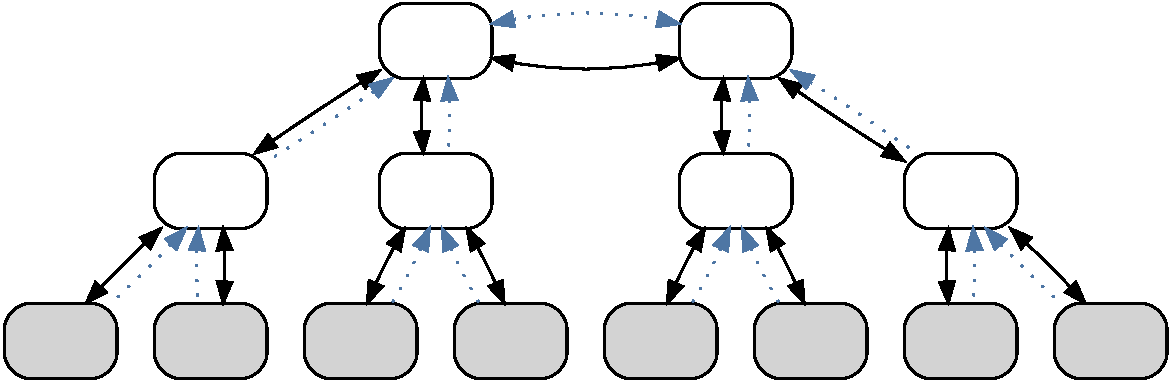
\includegraphics[width=.8\textwidth]{resources/images/example3}
    \caption{Choice of verification and validation techniques~\cite{li2002design}}\label{sec:eval:tec}
\end{figure}

\sidenote{Approaches}
\todomid{write}

\sidenote{Structure of Research}
\todomid{write about \Cref{fig:hourglass:evaluation}}

\begin{figure}[htpb]
    \centering
    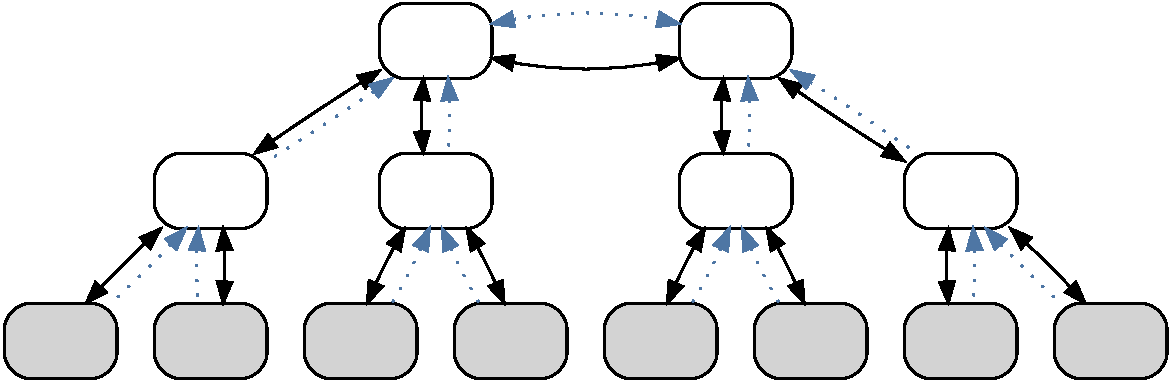
\includegraphics[width=.55\textwidth]{resources/images/example3}
    \caption{Placement of the evaluation in the structure of research}\label{fig:hourglass:evaluation}
\end{figure}

\section{Experimental Validation}

\sidenote{Overview}
\todomid{write about \Cref{tbl:eval:experiments}}

\begin{sidewaystable}
      \centering
      \captionsetup{type=table}
      \caption{Sideways table}
      \begin{tabular}{lllllll}\toprule
  \textbf{Experiment 1}   & \textbf{Experiment 2}  & \textbf{Experiment 3} & \textbf{Experiment 4} & \textbf{Experiment 5} & \textbf{Experiment 6} & \textbf{Experiment 7}  \\ \midrule
  CATCH & ME & IF & YOU & CAN & \emph{NOW} & OR NEVER \\
  CATCH & ME & IF & YOU & CAN & \emph{NOW} & OR NEVER \\
  CATCH & ME & IF & YOU & CAN & \emph{NOW} & OR NEVER \\
  CATCH & ME & IF & YOU & CAN & \emph{NOW} & OR NEVER \\
  CATCH & ME & IF & YOU & CAN & \emph{NOW} & OR NEVER \\
  CATCH & ME & IF & YOU & CAN & \emph{NOW} & OR NEVER \\
  CATCH & ME & IF & YOU & CAN & \emph{NOW} & OR NEVER \\
  CATCH & ME & IF & YOU & CAN & \emph{NOW} & OR NEVER \\
  CATCH & ME & IF & YOU & CAN & \emph{NOW} & OR NEVER \\
  CATCH & ME & IF & YOU & CAN & \emph{NOW} & OR NEVER \\
  CATCH & ME & IF & YOU & CAN & \emph{NOW} & OR NEVER \\
  \bottomrule
      \end{tabular}\label{tbl:eval:experiments}
\end{sidewaystable}


\subsection{Setup 1}

\sidenote{Overview}
\todomid{write}

\sidenote{Integration}
\todomid{write about \Cref{eq:var_idb}}

\small
\begin{equation}
  \begin{array}{l}
    \displaystyle t^{p_d}_{fw}(d) = \max_{d}(t_{child_{i}}) \\
    \displaystyle t^{p_d}_{db}(d) = \sum_{i=1}^{d} t_{db_{i}} \\
    \displaystyle t^{p_d}_{pc}(n,d) =
    	\begin{cases}
        	t_{pc}(d) + c(n) & \text{if $d = 1$,}\\
        	t_{pc}(d) + c(n) + \max(t_{avail}(d)) & \text{if $d>1$.}\\
        \end{cases}
  \end{array}\label{eq:var_idb}
\end{equation}
\normalsize

\sidenote{Example}
\todomid{write about \Cref{lst:eval:exp1}}

\needspace{5\baselineskip}\lstset{caption=Experiment 1, label=lst:eval:exp1,
language=ttl, breaklines=true, numbers=left,
stepnumber=1, frame=single, inputencoding=utf8/latin1}~\lstinputlisting{resources/code/example.java}

\subsection{Setup 2}

\sidenote{Overview}
\todomid{write}

\sidenote{Integration}
\todomid{write}

\sidenote{Example}
\todomid{write about \Cref{fig:eval:sub1,fig:eval:sub2,fig:eval:sub}}

\begin{figure}
    \begin{subfigure}[b]{.455\textwidth}
      \centering
      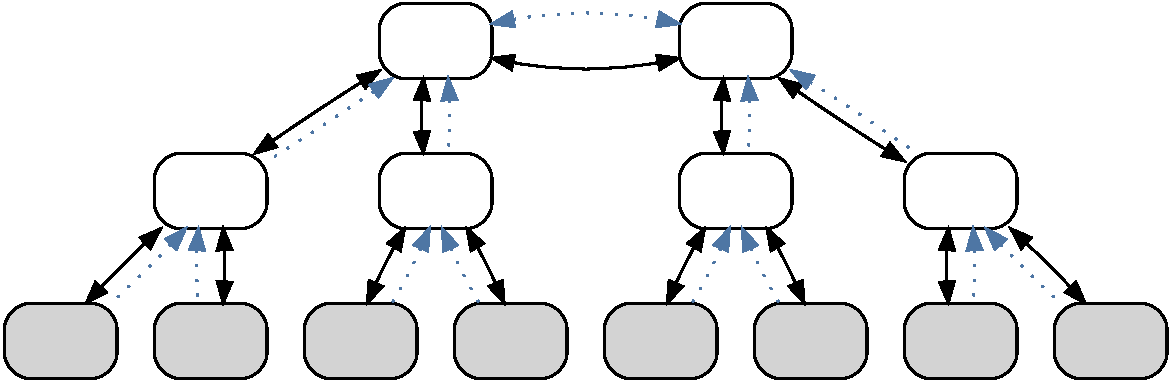
\includegraphics[width=.9\textwidth,frame]{resources/images/example3}
      \caption{Subfig 1}\label{fig:eval:sub1}
    \end{subfigure}~\begin{subfigure}[b]{.545\textwidth}
      \centering
      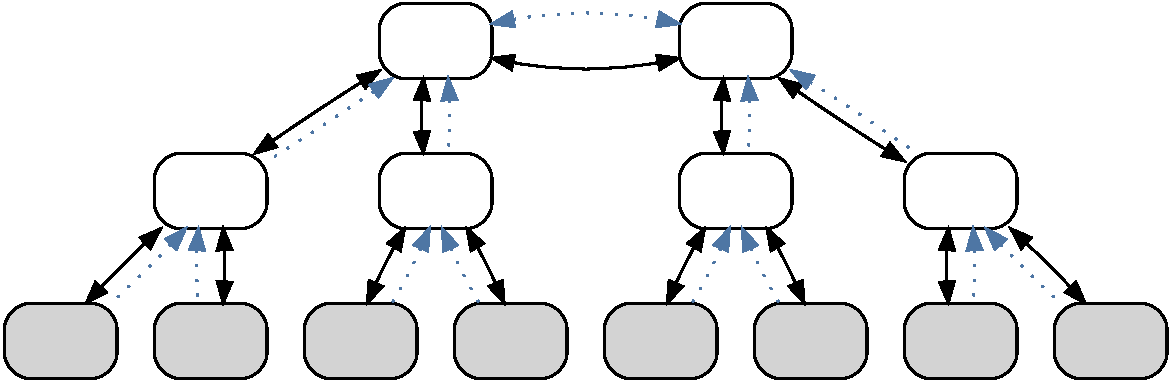
\includegraphics[width=1\textwidth,frame]{resources/images/example3}
      \caption{Subfig 2}\label{fig:eval:sub2}
    \end{subfigure}
    \caption{Sub Figures}\label{fig:eval:sub}
\end{figure}


\section{Performance Evaluation}

\sidenote{Overview}
\todomid{write}

\subsection{Evaluation 1}

\sidenote{Setup}
\todomid{write}

\sidenote{Cost Metrics}
\todomid{write}

\sidenote{Optimizing}
\todomid{write}

\sidenote{Performance Comparison}
\todomid{write}

\subsection{Evaluation 2}

\sidenote{Setup}
\todomid{write}

\sidenote{Response Times}
\todomid{write}
\begin{itemize}[noitemsep]
  \item \emph{In}: 159 ms $\pm$ 21 ms (95\% CI)
  \item \emph{Out}: 33 ms $\pm$ 5 ms (95\% CI)
  \item \emph{Between}: 238 ms $\pm$ 9 ms (95\% CI)
  \item \emph{After}: 45 ms $\pm$ 1 ms (95\% CI)
  \item \emph{Under}: 215 ms $\pm$ 2 ms (95\% CI)
  \item \emph{Over}: 148 ms $\pm$ 3 ms (95\% CI)
\end{itemize}

\sidenote{Scalability}
\todomid{write}

\section{Observational Validation}

\sidenote{Overview}
\todomid{write}

\subsection{Project 1}

\sidenote{Overview}
\todomid{write}

\sidenote{System Specification}
\todomid{write}

\sidenote{Extraction}
\todomid{write}

\sidenote{Example}
\todomid{write}

\subsection{Project 2}

\sidenote{Overview}
\todomid{write}

\sidenote{System Specification}
\todomid{write about \Cref{fig:eval:side}}

\begin{figure}[htbp]
    \centering
    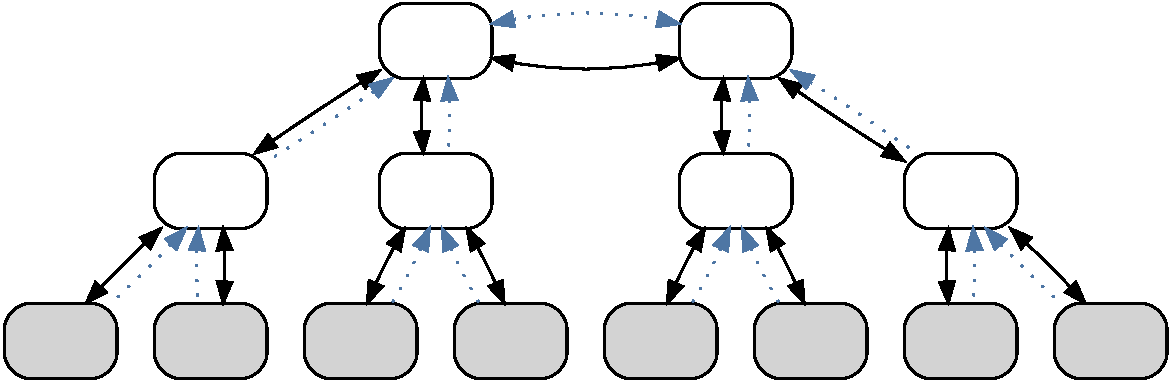
\includegraphics[height=.5\textwidth,angle=270]{resources/images/example3}
    \caption{Sideways figure}\label{fig:eval:side}
\end{figure}

\sidenote{Extraction}
\todomid{write}

\sidenote{Example}
\todomid{write}

\section{Deployments}

\sidenote{Overview}
\todomid{write}

\subsection{Installation 1}

\sidenote{Overview}
\todomid{write}

\sidenote{Integration}
\todomid{write}


\subsection{Installation 2}

\sidenote{Overview}
\todomid{write}

\sidenote{Integration}
\todomid{write}

\section{Code Verification}

\sidenote{Overview}
\todomid{write}

\sidenote{Static Tests}
\todomid{write}

\sidenote{Continuous Integration}
\todomid{write}

\sidenote{Test Coverage}
\todomid{write}

\section{Comparative Analysis}

\sidenote{Overview}
\todomid{write}

\subsection{Requirement Evaluation}

\sidenote{\Cref{tbl:reqs:compare}}
\todomid{write}

\begin{tabularx}{\textwidth}{p{2cm}X}
    \caption{Mapping requirements against own approach}\label{tbl:reqs:compare}\\
    \toprule
    \textbf{Requirements}& \textbf{Approach}  \\\midrule
    \endfirsthead%
    \toprule
    \textbf{Requirements}& \textbf{Approach}  \\\midrule
    \endhead%
\ref{req:stakeholder1:foo}\newline(Foo) &
\todomid{write}
\\\midrule

\ref{req:stakeholder1:bar}\newline(Bar) &
\todomid{write}
\\\midrule

\ref{req:stakeholder2:foo}\newline(Foo) &
\todomid{write}
\\\midrule

\ref{req:stakeholder2:bar}\newline(Bar) &
\todomid{write}
\\\midrule

\ref{req:stakeholder3:foo}\newline(Foo) &
\todomid{write}
\\\midrule

\ref{req:stakeholder3:bar}\newline(Bar) &
\todomid{write}

\\\bottomrule
\end{tabularx}

\subsection{Comparison with Other Approaches}

\sidenote{Overview}
\todomid{write}

\sidenote{\Cref{tbl:approaches:compare}}
\todomid{write about \Cref{tbl:approaches:compare}}

\begin{tabularx}{\textwidth}{p{2cm}LLLLLL}
    \caption{Comparison of related work with own approach}\label{tbl:approaches:compare}\\
    \toprule
    \textbf{Requirements} & \textbf{Related 1} & \textbf{Related 2} & \textbf{Related 3} & \textbf{Related 4} & \textbf{Related 5} & \textbf{Own Approach} \\\midrule
    \endfirsthead%
    \toprule
    \textbf{Requirements} & \textbf{Related 1} & \textbf{Related 2} & \textbf{Related 3} & \textbf{Related 4} & \textbf{Related 5} & \textbf{Own Approach} \\\midrule
    \endhead%

\ref{req:stakeholder1:foo}~\ref{req:stakeholder1:bar} & \textbf{(+)} & \textbf{(++)} & \textbf{(o)} & \textbf{(-)} & \textbf{(o)} & \textbf{(+++)} \\
(\ac{ABAC}) & \ac{ABAC} \ac{ABAC} v3, \ac{ABAC} \ac{ABAC} & \ac{ABAC} \ac{ABAC} v2, \ac{ABAC}, native \ac{ABAC} & \ac{ABAC} & native \ac{ABAC} & \ac{ABAC} \ac{ABAC} v2 & \ac{ABAC} \ac{ABAC} v3, \ac{ABAC} \ac{ABAC}, \ac{ABAC}, native \ac{ABAC}, native \\\midrule

\ref{req:stakeholder3:foo} & \textbf{(o)} & \textbf{(++)} &  & & \textbf{(++)} & \textbf{(+)} \\
(Details) & via foo & by bar / role-foo & --- & --- & bar / foo & foo-bar \\\midrule

\ref{req:stakeholder2:foo}~\ref{req:stakeholder2:bar}~\ref{req:stakeholder3:bar} & \textbf{(+)} & \textbf{(+)} & & \textbf{(+)} & \textbf{(+)} & \textbf{(+)} \\
(Barli) & via barli & via fooli & --- & via bar-foo & via foo-bar & via bar-bar \\\bottomrule
\end{tabularx}

\section{Conclusion}

\sidenote{Summary}
\todomid{write}

\sidenote{Takeaway 1}
\todomid{write}

\sidenote{Takeaway 2}
\todomid{write}

\sidenote{Takeaway 3}
\todomid{write}

\sidenote{Next chapter}
\todomid{write}

    % \cleardoublepage
\chapter{Summary and Further Work}\minitoc\label{sec:summary}\vspace{.5cm}

\section{Overview}

\begin{wrapfigure}{r}{0.2\textwidth}
    \centering
    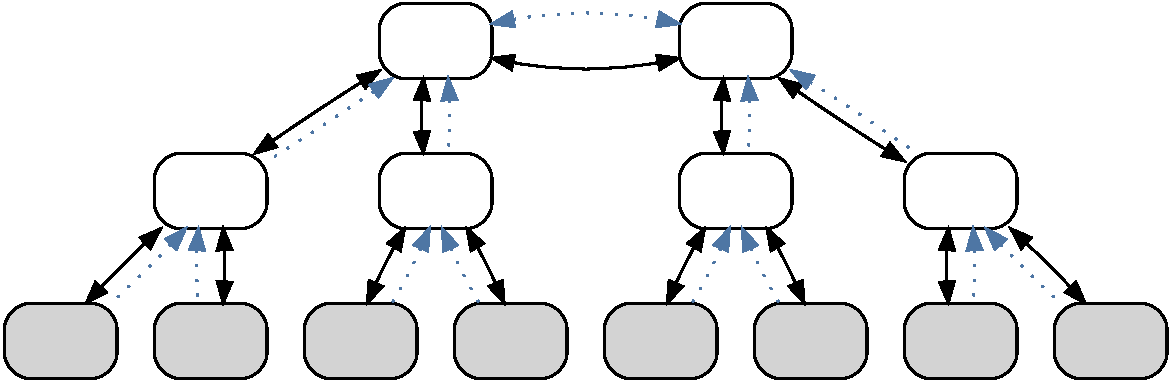
\includegraphics[width=0.2\textwidth]{resources/images/example3}
\end{wrapfigure}

\sidenote{Contributions}
\todomid{write}

\begin{figure}
    \centering
    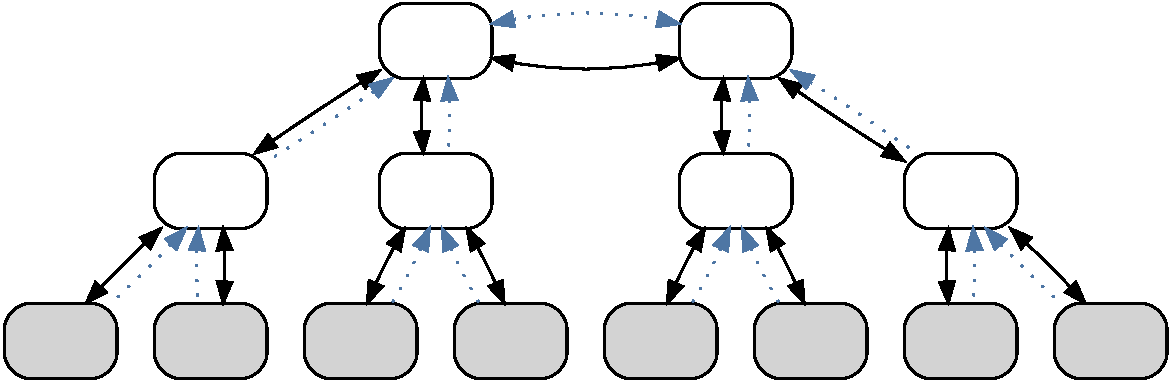
\includegraphics[width=.55\textwidth]{resources/images/example3}
    \caption{Placement of the outlook in the structure of research}\label{fig:hourglass:outlook}
\end{figure}

\sidenote{Dissemination}
\todomid{write about \Cref{fig:hourglass:outlook}}

\section{Conclusions and Impact}

\sidenote{Context}
\todomid{write}

\sidenote{Contribution 1}
\todomid{write}

\sidenote{Contribution 2}
\todomid{write}

\sidenote{Contribution 3}
\todomid{write}

\section{Outlook}

\sidenote{Intro}
\todomid{write}

\sidenote{Application Area 1}
\todomid{write about \Cref{fig:outlook:aa1}}

\begin{figure}
    \centering
    \includegraphics[width=.85\textwidth]{resources/images/example3}
    \caption{Area 1~\cite{li2002design}}\label{fig:outlook:aa1}
\end{figure}

\sidenote{Application Area 2}
\todomid{write}

\sidenote{Application Area 3}
\todomid{write}

\sidenote{Application Area 4}
\todomid{write}

    \nolinenumbers
    \cleardoublepage

    \appendix
    \pagenumbering{Roman}
    \setcounter{page}{1}
    % \cleardoublepage\chapter{Specifications}\minitoc\vspace{.5cm}

\section{Specification 1}\index{Specification 1}

\todomid{write about \Cref{lst:spec1}}

\lstset{language=ttl, breaklines=true, caption=Specification 1, %
emptylines=0,
label=lst:spec1, numbers=left, stepnumber=1, inputencoding=utf8}
\lstinputlisting{resources/code/example.java}


\section{Specification 2}\index{Specification 2}

\todomid{write about \Cref{lst:spec2}}

\lstset{language=ttl, breaklines=true, caption=Specification 2, %
emptylines=0,
label=lst:spec2, numbers=left, stepnumber=1, inputencoding=utf8}
\lstinputlisting{resources/code/example.java}


\cleardoublepage\chapter{Test Results}\minitoc\vspace{.5cm}

\section{Conformance Results}

\sidenote{Overview}
\todomid{write about \Cref{fig:test:result1,fig:test:result2}}

\begin{figure}[H]
    \centering
    \includegraphics[width=.9\textwidth,frame,page=1]{resources/images/example3}
    \caption{Test results (page 1)}\label{fig:test:result1}
\end{figure}

\begin{figure}[H]
    \centering
    \includegraphics[width=.9\textwidth,frame,page=1]{resources/images/example3}
    \caption{Test results (page 2)}\label{fig:test:result2}
\end{figure}

\section{Performance Results}

\subsection{Histograms}

\sidenote{Overview}
\todomid{write about \Cref{fig:eval:perf:hist:forms}}

\begin{figure}[H]
    \begin{subfigure}[b]{.5\textwidth}
      \centering
      \includegraphics[width=.95\textwidth,frame]{resources/images/example3}
      \caption{Form A}
    \end{subfigure}~\begin{subfigure}[b]{.5\textwidth}
      \centering
      \includegraphics[width=.95\textwidth,frame]{resources/images/example3}
      \caption{Form B}
    \end{subfigure}
    \caption{Histogram of Forms}\label{fig:eval:perf:hist:forms}
\end{figure}


\subsection{Lineplots}

\sidenote{Overview}
\todomid{write about \Cref{fig:eval:perf:line:lines}}

\begin{figure}[H]
    \begin{subfigure}[b]{.5\textwidth}
      \centering
      \includegraphics[width=.95\textwidth,frame]{resources/images/example3}
      \caption{Lines A}
    \end{subfigure}~\begin{subfigure}[b]{.5\textwidth}
      \centering
      \includegraphics[width=.95\textwidth,frame]{resources/images/example3}
      \caption{Lines A}
    \end{subfigure}
    \caption{Lineplot of the lines}\label{fig:eval:perf:line:lines}
\end{figure}


    \cleardoublepage
    % \cleardoublepage
\chapter*{Acronyms}
\mtcaddchapter\addstarredchapter{Acronyms}
\markboth{Acronyms}{Acronyms}
\stepcounter{chapter}
\renewcommand*{\chapterthumbformat}{Acronyms}
\printacronyms[name={}, exclude=exclude]

% \cleardoublepage
\stepcounter{chapter}
\renewcommand{\glossaryname}{Glossary}
\markboth{\glossaryname}{\glossaryname}
\renewcommand*{\chapterthumbformat}{\glossaryname}
\printglossary%

% \cleardoublepage
\chapter*{Bibliography}
\mtcaddchapter\addstarredchapter{Bibliography}
\markboth{Bibliography}{Bibliography}
\stepcounter{chapter}
\renewcommand*{\chapterthumbformat}{Bibliography}
\minitoc\vspace{.5cm}

\section*{List of Author's Publications Covered in this Thesis}
\nocite{li2002design}
\newrefcontext[labelprefix=a]
\printbibliography[keyword=own,heading=empty,category=cited]

\section*{References to Books}
\defbibfilter{books}{
  type=book
}
\newrefcontext[labelprefix=b]
\printbibliography[filter=books,heading=empty,category=cited,notkeyword=own]

\section*{References to Scientific Publications}
\defbibfilter{papers}{
  type=article
  or type=inproceedings
  or type=proceedings
  or type=journal
  or type=phdthesis
  or type=incollection
  % or type=book
  or keyword=thesis
  and not keyword=W3C
  and not keyword=RFC
  and not keyword=ITU
  and not keyword=IEEE
  and not keyword=ANSI
  and not keyword=OGF
  and not keyword=web
  and not keyword=presentation
  and not keyword=workingpaper
}
\newrefcontext[labelprefix=p]
\printbibliography[filter=papers,heading=empty,category=cited,notkeyword=own]


\section*{Technical References}

\defbibfilter{standards}{
  type=techreport
  or type=report
  or keyword=W3C
  or keyword=RFC
  or keyword=TMF
  or keyword=ITU
  or keyword=IEEE
  or keyword=ANSI
  or keyword=OGF
  or keyword=ETSI
  or keyword=OneM2M
  or keyword=IETF
  or keyword=OMA
  or keyword=TMG
  or keyword=NIST
  or keyword=SNIA
  or keyword=OMG
  or keyword=DMTF
  or keyword=OASIS
  or keyword=deliverable
  or keyword=techreport
  or keyword=whitepaper
  and not keyword=web
  and not keyword=presentation
  and not keyword=workingpaper
}
\newrefcontext[labelprefix=t]
\printbibliography[filter=standards,heading=empty,category=cited,notkeyword=own]


\section*{Miscellaneous References}
\defbibfilter{misc}{
  keyword=web
  or keyword=presentation
  or keyword=workingpaper
}
\newrefcontext[labelprefix=m]
\printbibliography[filter=misc,heading=empty,category=cited,notkeyword=own]


% \section*{Not referenced (will be empty)}
% \todo{this section should be empty at the end}
% \nocite{*}
% \newrefcontext[labelprefix=x]
% \printbibliography[heading=empty,notcategory=cited,notkeyword=own]


    \backmatter
    \cleardoublepage% \cleardoublepage
\phantomsection
\stepcounter{chapter}
\renewcommand{\indexname}{Index}
\renewcommand*{\chapterthumbformat}{\indexname}
\markboth{\indexname}{\indexname}
\printindex%

\end{document}
% ------------------------------------------------------------------------------
